\documentclass[twoside]{book}

% Packages required by doxygen
\usepackage{fixltx2e}
\usepackage{calc}
\usepackage{doxygen}
\usepackage[export]{adjustbox} % also loads graphicx
\usepackage{graphicx}
\usepackage[utf8]{inputenc}
\usepackage{makeidx}
\usepackage{multicol}
\usepackage{multirow}
\PassOptionsToPackage{warn}{textcomp}
\usepackage{textcomp}
\usepackage[nointegrals]{wasysym}
\usepackage[table]{xcolor}

% Font selection
\usepackage[T1]{fontenc}
\usepackage[scaled=.90]{helvet}
\usepackage{courier}
\usepackage{amssymb}
\usepackage{sectsty}
\renewcommand{\familydefault}{\sfdefault}
\allsectionsfont{%
  \fontseries{bc}\selectfont%
  \color{darkgray}%
}
\renewcommand{\DoxyLabelFont}{%
  \fontseries{bc}\selectfont%
  \color{darkgray}%
}
\newcommand{\+}{\discretionary{\mbox{\scriptsize$\hookleftarrow$}}{}{}}

% Page & text layout
\usepackage{geometry}
\geometry{%
  a4paper,%
  top=2.5cm,%
  bottom=2.5cm,%
  left=2.5cm,%
  right=2.5cm%
}
\tolerance=750
\hfuzz=15pt
\hbadness=750
\setlength{\emergencystretch}{15pt}
\setlength{\parindent}{0cm}
\setlength{\parskip}{3ex plus 2ex minus 2ex}
\makeatletter
\renewcommand{\paragraph}{%
  \@startsection{paragraph}{4}{0ex}{-1.0ex}{1.0ex}{%
    \normalfont\normalsize\bfseries\SS@parafont%
  }%
}
\renewcommand{\subparagraph}{%
  \@startsection{subparagraph}{5}{0ex}{-1.0ex}{1.0ex}{%
    \normalfont\normalsize\bfseries\SS@subparafont%
  }%
}
\makeatother

% Headers & footers
\usepackage{fancyhdr}
\pagestyle{fancyplain}
\fancyhead[LE]{\fancyplain{}{\bfseries\thepage}}
\fancyhead[CE]{\fancyplain{}{}}
\fancyhead[RE]{\fancyplain{}{\bfseries\leftmark}}
\fancyhead[LO]{\fancyplain{}{\bfseries\rightmark}}
\fancyhead[CO]{\fancyplain{}{}}
\fancyhead[RO]{\fancyplain{}{\bfseries\thepage}}
\fancyfoot[LE]{\fancyplain{}{}}
\fancyfoot[CE]{\fancyplain{}{}}
\fancyfoot[RE]{\fancyplain{}{\bfseries\scriptsize Generated by Doxygen }}
\fancyfoot[LO]{\fancyplain{}{\bfseries\scriptsize Generated by Doxygen }}
\fancyfoot[CO]{\fancyplain{}{}}
\fancyfoot[RO]{\fancyplain{}{}}
\renewcommand{\footrulewidth}{0.4pt}
\renewcommand{\chaptermark}[1]{%
  \markboth{#1}{}%
}
\renewcommand{\sectionmark}[1]{%
  \markright{\thesection\ #1}%
}

% Indices & bibliography
\usepackage{natbib}
\usepackage[titles]{tocloft}
\setcounter{tocdepth}{3}
\setcounter{secnumdepth}{5}
\makeindex

% Hyperlinks (required, but should be loaded last)
\usepackage{ifpdf}
\ifpdf
  \usepackage[pdftex,pagebackref=true]{hyperref}
\else
  \usepackage[ps2pdf,pagebackref=true]{hyperref}
\fi
\hypersetup{%
  colorlinks=true,%
  linkcolor=blue,%
  citecolor=blue,%
  unicode%
}

% Custom commands
\newcommand{\clearemptydoublepage}{%
  \newpage{\pagestyle{empty}\cleardoublepage}%
}

\usepackage{caption}
\captionsetup{labelsep=space,justification=centering,font={bf},singlelinecheck=off,skip=4pt,position=top}

%===== C O N T E N T S =====

\begin{document}

% Titlepage & ToC
\hypersetup{pageanchor=false,
             bookmarksnumbered=true,
             pdfencoding=unicode
            }
\pagenumbering{alph}
\begin{titlepage}
\vspace*{7cm}
\begin{center}%
{\Large Lab\+Robotics\+Project }\\
\vspace*{1cm}
{\large Generated by Doxygen 1.8.14}\\
\end{center}
\end{titlepage}
\clearemptydoublepage
\pagenumbering{roman}
\tableofcontents
\clearemptydoublepage
\pagenumbering{arabic}
\hypersetup{pageanchor=true}

%--- Begin generated contents ---
\chapter{Class Index}
\section{Class List}
Here are the classes, structs, unions and interfaces with brief descriptions\+:\begin{DoxyCompactList}
\item\contentsline{section}{\mbox{\hyperlink{class_angle}{Angle}} \\*This class allows to save and handle angles. It supports D\+EG and R\+AD, operations such as addition and subtraction with operators overloading, conversion from R\+AD to D\+EG and viceversa and normalization of the angle }{\pageref{class_angle}}{}
\item\contentsline{section}{\mbox{\hyperlink{class_cal_settings}{Cal\+Settings}} }{\pageref{class_cal_settings}}{}
\item\contentsline{section}{\mbox{\hyperlink{class_camera_capture}{Camera\+Capture}} }{\pageref{class_camera_capture}}{}
\item\contentsline{section}{\mbox{\hyperlink{class_clipper_lib_1_1_clipper}{Clipper\+Lib\+::\+Clipper}} }{\pageref{class_clipper_lib_1_1_clipper}}{}
\item\contentsline{section}{\mbox{\hyperlink{class_clipper_lib_1_1_clipper_base}{Clipper\+Lib\+::\+Clipper\+Base}} }{\pageref{class_clipper_lib_1_1_clipper_base}}{}
\item\contentsline{section}{\mbox{\hyperlink{class_clipper_lib_1_1clipper_exception}{Clipper\+Lib\+::clipper\+Exception}} }{\pageref{class_clipper_lib_1_1clipper_exception}}{}
\item\contentsline{section}{\mbox{\hyperlink{class_clipper_lib_1_1_clipper_offset}{Clipper\+Lib\+::\+Clipper\+Offset}} }{\pageref{class_clipper_lib_1_1_clipper_offset}}{}
\item\contentsline{section}{\mbox{\hyperlink{class_configuration2}{Configuration2$<$ T1 $>$}} \\*This class stores a configuration, that is a point and an angle }{\pageref{class_configuration2}}{}
\item\contentsline{section}{\mbox{\hyperlink{class_curve}{Curve$<$ T $>$}} }{\pageref{class_curve}}{}
\item\contentsline{section}{\mbox{\hyperlink{struct_clipper_lib_1_1_double_point}{Clipper\+Lib\+::\+Double\+Point}} }{\pageref{struct_clipper_lib_1_1_double_point}}{}
\item\contentsline{section}{\mbox{\hyperlink{class_dubins}{Dubins$<$ T $>$}} \\*Class to store a \mbox{\hyperlink{class_dubins}{Dubins}} curve. This class inherits from {\ttfamily \mbox{\hyperlink{class_curve}{Curve}}} and is composed of three {\ttfamily \mbox{\hyperlink{class_dubins_arc}{Dubins\+Arc}}} }{\pageref{class_dubins}}{}
\item\contentsline{section}{\mbox{\hyperlink{class_dubins_arc}{Dubins\+Arc$<$ T1, T2 $>$}} \\*Class to store a maneuver of \mbox{\hyperlink{class_dubins}{Dubins}}. It inherits from {\ttfamily \mbox{\hyperlink{class_curve}{Curve}}}. Since each \mbox{\hyperlink{class_dubins}{Dubins}} is formed of atmost 3 maneuvers, this class is meant to store one of this maneuver, which can be L, R or S respectively Left, Right, Straight }{\pageref{class_dubins_arc}}{}
\item\contentsline{section}{\mbox{\hyperlink{class_dubins_set}{Dubins\+Set$<$ T $>$}} \\*Given a set of point, compute the shortest set of \mbox{\hyperlink{class_dubins}{Dubins}} that allows to go from start to end through all points }{\pageref{class_dubins_set}}{}
\item\contentsline{section}{\mbox{\hyperlink{class_filter}{Filter}} }{\pageref{class_filter}}{}
\item\contentsline{section}{\mbox{\hyperlink{class_gate}{Gate}} }{\pageref{class_gate}}{}
\item\contentsline{section}{\mbox{\hyperlink{struct_camera_capture_1_1input__options__t}{Camera\+Capture\+::input\+\_\+options\+\_\+t}} \\*Structure for store the input option for the class \mbox{\hyperlink{class_camera_capture}{Camera\+Capture}} }{\pageref{struct_camera_capture_1_1input__options__t}}{}
\item\contentsline{section}{\mbox{\hyperlink{class_clipper_lib_1_1_int128}{Clipper\+Lib\+::\+Int128}} }{\pageref{class_clipper_lib_1_1_int128}}{}
\item\contentsline{section}{\mbox{\hyperlink{struct_clipper_lib_1_1_intersect_node}{Clipper\+Lib\+::\+Intersect\+Node}} }{\pageref{struct_clipper_lib_1_1_intersect_node}}{}
\item\contentsline{section}{\mbox{\hyperlink{struct_clipper_lib_1_1_int_point}{Clipper\+Lib\+::\+Int\+Point}} }{\pageref{struct_clipper_lib_1_1_int_point}}{}
\item\contentsline{section}{\mbox{\hyperlink{struct_clipper_lib_1_1_int_rect}{Clipper\+Lib\+::\+Int\+Rect}} }{\pageref{struct_clipper_lib_1_1_int_rect}}{}
\item\contentsline{section}{\mbox{\hyperlink{struct_clipper_lib_1_1_join}{Clipper\+Lib\+::\+Join}} }{\pageref{struct_clipper_lib_1_1_join}}{}
\item\contentsline{section}{\mbox{\hyperlink{struct_clipper_lib_1_1_local_minimum}{Clipper\+Lib\+::\+Local\+Minimum}} }{\pageref{struct_clipper_lib_1_1_local_minimum}}{}
\item\contentsline{section}{\mbox{\hyperlink{struct_clipper_lib_1_1_loc_min_sorter}{Clipper\+Lib\+::\+Loc\+Min\+Sorter}} }{\pageref{struct_clipper_lib_1_1_loc_min_sorter}}{}
\item\contentsline{section}{\mbox{\hyperlink{class_mapp}{Mapp}} }{\pageref{class_mapp}}{}
\item\contentsline{section}{\mbox{\hyperlink{class_my_exception}{My\+Exception$<$ T $>$}} }{\pageref{class_my_exception}}{}
\item\contentsline{section}{\mbox{\hyperlink{class_object}{Object}} }{\pageref{class_object}}{}
\item\contentsline{section}{\mbox{\hyperlink{class_obstacle}{Obstacle}} }{\pageref{class_obstacle}}{}
\item\contentsline{section}{\mbox{\hyperlink{struct_clipper_lib_1_1_out_pt}{Clipper\+Lib\+::\+Out\+Pt}} }{\pageref{struct_clipper_lib_1_1_out_pt}}{}
\item\contentsline{section}{\mbox{\hyperlink{struct_clipper_lib_1_1_out_rec}{Clipper\+Lib\+::\+Out\+Rec}} }{\pageref{struct_clipper_lib_1_1_out_rec}}{}
\item\contentsline{section}{\mbox{\hyperlink{class_point2}{Point2$<$ T $>$}} \\*Class that stores two value to construct a point in 2D. The value is saved in a \mbox{\hyperlink{class_tuple}{Tuple}} }{\pageref{class_point2}}{}
\item\contentsline{section}{\mbox{\hyperlink{class_clipper_lib_1_1_poly_node}{Clipper\+Lib\+::\+Poly\+Node}} }{\pageref{class_clipper_lib_1_1_poly_node}}{}
\item\contentsline{section}{\mbox{\hyperlink{class_clipper_lib_1_1_poly_tree}{Clipper\+Lib\+::\+Poly\+Tree}} }{\pageref{class_clipper_lib_1_1_poly_tree}}{}
\item\contentsline{section}{\mbox{\hyperlink{class_robot_project}{Robot\+Project}} }{\pageref{class_robot_project}}{}
\item\contentsline{section}{\mbox{\hyperlink{class_settings}{Settings}} }{\pageref{class_settings}}{}
\item\contentsline{section}{\mbox{\hyperlink{struct_clipper_lib_1_1_t_edge}{Clipper\+Lib\+::\+T\+Edge}} }{\pageref{struct_clipper_lib_1_1_t_edge}}{}
\item\contentsline{section}{\mbox{\hyperlink{class_tuple}{Tuple$<$ T $>$}} }{\pageref{class_tuple}}{}
\item\contentsline{section}{\mbox{\hyperlink{class_victim}{Victim}} }{\pageref{class_victim}}{}
\end{DoxyCompactList}

\chapter{File Index}
\section{File List}
Here is a list of all files with brief descriptions\+:\begin{DoxyCompactList}
\item\contentsline{section}{src/\mbox{\hyperlink{calibration_8cc}{calibration.\+cc}} }{\pageref{calibration_8cc}}{}
\item\contentsline{section}{src/\mbox{\hyperlink{calibration_8hh}{calibration.\+hh}} \\*Library for calibration }{\pageref{calibration_8hh}}{}
\item\contentsline{section}{src/\mbox{\hyperlink{calibration__run_8cc}{calibration\+\_\+run.\+cc}} }{\pageref{calibration__run_8cc}}{}
\item\contentsline{section}{src/\mbox{\hyperlink{create__xml_8cc}{create\+\_\+xml.\+cc}} }{\pageref{create__xml_8cc}}{}
\item\contentsline{section}{src/\mbox{\hyperlink{detection_8cc}{detection.\+cc}} }{\pageref{detection_8cc}}{}
\item\contentsline{section}{src/\mbox{\hyperlink{detection_8hh}{detection.\+hh}} }{\pageref{detection_8hh}}{}
\item\contentsline{section}{src/\mbox{\hyperlink{detection__run_8cc}{detection\+\_\+run.\+cc}} }{\pageref{detection__run_8cc}}{}
\item\contentsline{section}{src/\mbox{\hyperlink{main_8cc}{main.\+cc}} }{\pageref{main_8cc}}{}
\item\contentsline{section}{src/\mbox{\hyperlink{unwrapping_8cc}{unwrapping.\+cc}} }{\pageref{unwrapping_8cc}}{}
\item\contentsline{section}{src/\mbox{\hyperlink{unwrapping_8hh}{unwrapping.\+hh}} }{\pageref{unwrapping_8hh}}{}
\item\contentsline{section}{src/\mbox{\hyperlink{unwrapping__run_8cc}{unwrapping\+\_\+run.\+cc}} }{\pageref{unwrapping__run_8cc}}{}
\item\contentsline{section}{src/\mbox{\hyperlink{utils_8cc}{utils.\+cc}} }{\pageref{utils_8cc}}{}
\item\contentsline{section}{src/\mbox{\hyperlink{utils_8hh}{utils.\+hh}} }{\pageref{utils_8hh}}{}
\end{DoxyCompactList}

\chapter{Class Documentation}
\hypertarget{class_settings}{}\section{Settings Class Reference}
\label{class_settings}\index{Settings@{Settings}}


{\ttfamily \#include $<$settings.\+hh$>$}



Collaboration diagram for Settings\+:
\nopagebreak
\begin{figure}[H]
\begin{center}
\leavevmode
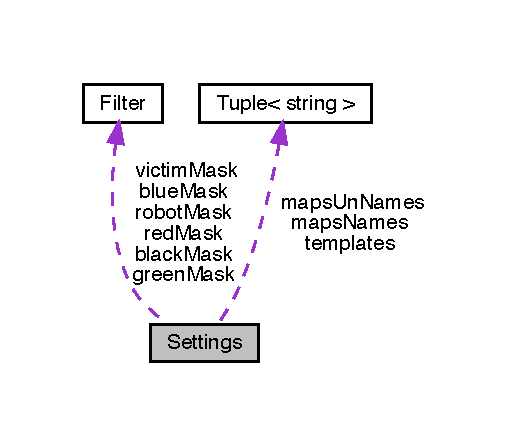
\includegraphics[width=244pt]{class_settings__coll__graph}
\end{center}
\end{figure}
\subsection*{Public Types}
\begin{DoxyCompactItemize}
\item 
enum \mbox{\hyperlink{class_settings_a30d85f2e06a54ae9bc8da2d01037658f}{C\+O\+L\+OR}} \{ \newline
\mbox{\hyperlink{class_settings_a30d85f2e06a54ae9bc8da2d01037658fad72cf235641afa26b82dc5bb8b0db4e1}{B\+L\+A\+CK}}, 
\mbox{\hyperlink{class_settings_a30d85f2e06a54ae9bc8da2d01037658fa164128164b54423f54968a67580a4ce3}{R\+ED}}, 
\mbox{\hyperlink{class_settings_a30d85f2e06a54ae9bc8da2d01037658fa79963b69fcbb589ae6f3f09ac6c5ae90}{G\+R\+E\+EN}}, 
\mbox{\hyperlink{class_settings_a30d85f2e06a54ae9bc8da2d01037658fab4951d8c5bc23e9dab4e9cb53ef3fb26}{V\+I\+C\+T\+I\+MS}}, 
\newline
\mbox{\hyperlink{class_settings_a30d85f2e06a54ae9bc8da2d01037658fa23f16922180d0f5fdc679584f75f83c3}{B\+L\+UE}}, 
\mbox{\hyperlink{class_settings_a30d85f2e06a54ae9bc8da2d01037658fa1cf089d6c6dda465fa704222461f0b28}{R\+O\+B\+OT}}
 \}
\end{DoxyCompactItemize}
\subsection*{Public Member Functions}
\begin{DoxyCompactItemize}
\item 
\mbox{\hyperlink{class_settings_a716069efb4808f2c395dfa218ec1c540}{Settings}} (string \+\_\+base\+Folder=\char`\"{}data/\char`\"{}, string \+\_\+maps\+Folder=\char`\"{}map\char`\"{}, string \+\_\+templates\+Folder=\char`\"{}num\+\_\+template/\char`\"{}, vector$<$ string $>$ \+\_\+maps\+Names=\{\}, vector$<$ string $>$ \+\_\+maps\+Un\+Names=\{\}, string \+\_\+intrinsic\+Calibration\+File=\char`\"{}intrinsic\+\_\+calibration.\+xml\char`\"{}, string \+\_\+calibration\+File=\char`\"{}calib\+\_\+config.\+xml\char`\"{}, Filter \+\_\+black\+Mask=\mbox{\hyperlink{class_filter}{Filter}}(0, 0, 0, 179, 255, 70), \mbox{\hyperlink{class_filter}{Filter}} \+\_\+red\+Mask=\mbox{\hyperlink{class_filter}{Filter}}(15, 100, 140, 160, 255, 255), \mbox{\hyperlink{class_filter}{Filter}} \+\_\+green\+Mask=\mbox{\hyperlink{class_filter}{Filter}}(54, 74, 25, 119, 255, 88), \mbox{\hyperlink{class_filter}{Filter}} \+\_\+victim\+Mask=\mbox{\hyperlink{class_filter}{Filter}}(0, 0, 0, 179, 255, 80), \mbox{\hyperlink{class_filter}{Filter}} \+\_\+blue\+Mask=\mbox{\hyperlink{class_filter}{Filter}}(100, 100, 40, 140, 200, 170), \mbox{\hyperlink{class_filter}{Filter}} \+\_\+robote\+Mask=\mbox{\hyperlink{class_filter}{Filter}}(100, 100, 40, 140, 200, 170), \mbox{\hyperlink{draw_8hh_aa620a13339ac3a1177c86edc549fda9b}{int}} \+\_\+kernel\+Side=9, string \+\_\+convex\+Hull\+File=\char`\"{}convex\+Hull.\+xml\char`\"{}, vector$<$ string $>$ \+\_\+templates=\{\})
\begin{DoxyCompactList}\small\item\em Constructor of class \mbox{\hyperlink{class_settings}{Settings}}. The value are all set by default. The constructor does N\+OT read from or write to file. \end{DoxyCompactList}\item 
\mbox{\hyperlink{class_settings_a4a65be5921dfc9fddc476e5320541d89}{$\sim$\+Settings}} ()
\begin{DoxyCompactList}\small\item\em Destructor. \end{DoxyCompactList}\item 
void \mbox{\hyperlink{class_settings_a14ebf63b888dd7ecf7a34de9eaba1ae8}{save}} (string \+\_\+base\+Folder=\char`\"{}data/\char`\"{}, string \+\_\+maps\+Folder=\char`\"{}map/\char`\"{}, string \+\_\+templates\+Folder=\char`\"{}num\+\_\+template/\char`\"{}, vector$<$ string $>$ \+\_\+maps\+Names=\{\}, vector$<$ string $>$ \+\_\+maps\+Un\+Names=\{\}, string \+\_\+intrinsic\+Calibration\+File=\char`\"{}intrinsic\+\_\+calibration.\+xml\char`\"{}, string \+\_\+calibration\+File=\char`\"{}calib\+\_\+config.\+xml\char`\"{}, Filter \+\_\+black\+Mask=\mbox{\hyperlink{class_filter}{Filter}}(0, 0, 0, 179, 255, 70), \mbox{\hyperlink{class_filter}{Filter}} \+\_\+red\+Mask=\mbox{\hyperlink{class_filter}{Filter}}(15, 100, 140, 160, 255, 255), \mbox{\hyperlink{class_filter}{Filter}} \+\_\+green\+Mask=\mbox{\hyperlink{class_filter}{Filter}}(54, 74, 25, 119, 255, 88), \mbox{\hyperlink{class_filter}{Filter}} \+\_\+victim\+Mask=\mbox{\hyperlink{class_filter}{Filter}}(0, 0, 0, 179, 255, 80), \mbox{\hyperlink{class_filter}{Filter}} \+\_\+blue\+Mask=\mbox{\hyperlink{class_filter}{Filter}}(100, 100, 40, 140, 200, 170), \mbox{\hyperlink{class_filter}{Filter}} \+\_\+robote\+Mask=\mbox{\hyperlink{class_filter}{Filter}}(100, 100, 40, 140, 200, 170), \mbox{\hyperlink{draw_8hh_aa620a13339ac3a1177c86edc549fda9b}{int}} \+\_\+kernel\+Side=9, string \+\_\+convex\+Hull\+File=\char`\"{}convex\+Hull.\+xml\char`\"{}, vector$<$ string $>$ \+\_\+templates=\{\})
\begin{DoxyCompactList}\small\item\em Function to change values. The value are all set by default. This function does N\+OT read from or write to file. \end{DoxyCompactList}\item 
void \mbox{\hyperlink{class_settings_a69b5dc81f8928efdcfc19e409f6015fb}{write\+To\+File}} (string \+\_\+path=\char`\"{}\char`\"{})
\begin{DoxyCompactList}\small\item\em Function to write settings to file. Default is data/settings.\+xml. \end{DoxyCompactList}\item 
void \mbox{\hyperlink{class_settings_a8491d82663ed43dadc540c4a402156fc}{read\+From\+File}} (string \+\_\+path=\char`\"{}\char`\"{})
\begin{DoxyCompactList}\small\item\em Function to read from file. The data found is going to be added to the settings. Default file is data/settings.\+xml. \end{DoxyCompactList}\item 
void \mbox{\hyperlink{class_settings_a8ad60105ab9848720d05ebd19c5063f2}{clean}} ()
\begin{DoxyCompactList}\small\item\em Function to clean all settings\+: number types are set to 0, string are set to \char`\"{}\char`\"{}, Tuples are set to Tuple$<$$>$() and \mbox{\hyperlink{class_filter}{Filter}} are set to all 0s. \end{DoxyCompactList}\item 
void \mbox{\hyperlink{class_settings_acd13c0d603d94c7c2da58cd92bc955c8}{clean\+And\+Read}} (string \+\_\+path=\char`\"{}\char`\"{})
\begin{DoxyCompactList}\small\item\em Function to clean all settings and then read from file. If no path is given the base\+Folder is used. \end{DoxyCompactList}\item 
\mbox{\hyperlink{class_tuple}{Tuple}}$<$ string $>$ \mbox{\hyperlink{class_settings_aa924e455cc6ac356ba6a4c59ab09591c}{maps}} (\mbox{\hyperlink{class_tuple}{Tuple}}$<$ \mbox{\hyperlink{draw_8hh_aa620a13339ac3a1177c86edc549fda9b}{int}} $>$ ids=\mbox{\hyperlink{class_tuple}{Tuple}}$<$ \mbox{\hyperlink{draw_8hh_aa620a13339ac3a1177c86edc549fda9b}{int}} $>$())
\begin{DoxyCompactList}\small\item\em Function to return the paths of maps. If ids are not specified all maps are returned. \end{DoxyCompactList}\item 
\mbox{\hyperlink{class_tuple}{Tuple}}$<$ string $>$ \mbox{\hyperlink{class_settings_adc050f187f4040f5e897b2ff41caedd0}{maps}} (\mbox{\hyperlink{draw_8hh_aa620a13339ac3a1177c86edc549fda9b}{int}} id=-\/1)
\begin{DoxyCompactList}\small\item\em Function to return the path of a map. If id is negative all maps are returned. \end{DoxyCompactList}\item 
string \mbox{\hyperlink{class_settings_aa34e6004beffad1bc5fd81f99353d3e1}{maps}} (string \+\_\+map\+Name)
\begin{DoxyCompactList}\small\item\em A function to return the path of a given map. \end{DoxyCompactList}\item 
\mbox{\hyperlink{class_tuple}{Tuple}}$<$ string $>$ \mbox{\hyperlink{class_settings_ab638c9895f57ed5e8ab64084752c660d}{maps}} (\mbox{\hyperlink{class_tuple}{Tuple}}$<$ string $>$ \+\_\+map\+Names)
\begin{DoxyCompactList}\small\item\em A function to return the paths of a given \mbox{\hyperlink{class_tuple}{Tuple}} of maps. \end{DoxyCompactList}\item 
bool \mbox{\hyperlink{class_settings_aeee4537bd39c18ca3a711a73c9c2277e}{add\+Un\+Map}} (string un\+Map)
\begin{DoxyCompactList}\small\item\em Adds the name of an undistorted map to the list. \end{DoxyCompactList}\item 
\mbox{\hyperlink{class_tuple}{Tuple}}$<$ string $>$ \mbox{\hyperlink{class_settings_a7cbf0234eaca6582ce982f0cf756d282}{un\+Maps}} (\mbox{\hyperlink{class_tuple}{Tuple}}$<$ \mbox{\hyperlink{draw_8hh_aa620a13339ac3a1177c86edc549fda9b}{int}} $>$ ids=\mbox{\hyperlink{class_tuple}{Tuple}}$<$ \mbox{\hyperlink{draw_8hh_aa620a13339ac3a1177c86edc549fda9b}{int}} $>$())
\begin{DoxyCompactList}\small\item\em Function to return the paths of undistorted maps. If ids are not specified all undistorted maps are returned. \end{DoxyCompactList}\item 
\mbox{\hyperlink{class_tuple}{Tuple}}$<$ string $>$ \mbox{\hyperlink{class_settings_a0619c378aff05b5762afe0280b40e07a}{un\+Maps}} (\mbox{\hyperlink{draw_8hh_aa620a13339ac3a1177c86edc549fda9b}{int}} id=-\/1)
\begin{DoxyCompactList}\small\item\em Function to return the path of an undistorted map. If id is negative all undistorted maps are returned. \end{DoxyCompactList}\item 
string \mbox{\hyperlink{class_settings_a6e62c5eb18f6abc4bcbcd11e018fda8b}{un\+Maps}} (string \+\_\+un\+Map\+Name)
\begin{DoxyCompactList}\small\item\em A function to return the path of a given undistorted map. \end{DoxyCompactList}\item 
\mbox{\hyperlink{class_tuple}{Tuple}}$<$ string $>$ \mbox{\hyperlink{class_settings_aa89550d142cb4101faf35af214f4edff}{un\+Maps}} (\mbox{\hyperlink{class_tuple}{Tuple}}$<$ string $>$ \+\_\+un\+Map\+Names)
\begin{DoxyCompactList}\small\item\em A function to return the paths of a given \mbox{\hyperlink{class_tuple}{Tuple}} of undistorted maps. \end{DoxyCompactList}\item 
\mbox{\hyperlink{class_tuple}{Tuple}}$<$ string $>$ \mbox{\hyperlink{class_settings_af68cb84ba3c8d21e004661fee7c0efe7}{get\+Templates}} (\mbox{\hyperlink{draw_8hh_aa620a13339ac3a1177c86edc549fda9b}{int}} id=-\/1)
\begin{DoxyCompactList}\small\item\em Function to return the path of a template. If id is negative all templates are returned. \end{DoxyCompactList}\item 
string \mbox{\hyperlink{class_settings_aa77f9d559fb0f14d551c4ee8a742e6b0}{get\+Templates}} (string \+\_\+template)
\begin{DoxyCompactList}\small\item\em A function to return the path of a given template. \end{DoxyCompactList}\item 
\mbox{\hyperlink{class_tuple}{Tuple}}$<$ string $>$ \mbox{\hyperlink{class_settings_a2fe58de6135c30ec02bccfc20cc15fe3}{get\+Templates}} (\mbox{\hyperlink{class_tuple}{Tuple}}$<$ string $>$ \+\_\+templates)
\begin{DoxyCompactList}\small\item\em A function to return the paths of a given \mbox{\hyperlink{class_tuple}{Tuple}} of templates. \end{DoxyCompactList}\item 
void \mbox{\hyperlink{class_settings_ad0d55c536a84990b048463b924c7d88e}{change\+Mask}} (\mbox{\hyperlink{class_tuple}{Tuple}}$<$ \mbox{\hyperlink{class_settings_a30d85f2e06a54ae9bc8da2d01037658f}{C\+O\+L\+OR}} $>$ color, \mbox{\hyperlink{class_tuple}{Tuple}}$<$ \mbox{\hyperlink{class_filter}{Filter}} $>$ fil)
\begin{DoxyCompactList}\small\item\em Change the values of \mbox{\hyperlink{class_tuple}{Tuple}} of filters. Mind that no write function is called. \end{DoxyCompactList}\item 
void \mbox{\hyperlink{class_settings_ad00eb6c82b7e6af5afbb8d881c50dea8}{change\+Mask}} (\mbox{\hyperlink{class_settings_a30d85f2e06a54ae9bc8da2d01037658f}{C\+O\+L\+OR}} color, \mbox{\hyperlink{class_filter}{Filter}} fil)
\begin{DoxyCompactList}\small\item\em Change the values of a filter. Mind that no write function is called. \end{DoxyCompactList}\item 
stringstream \mbox{\hyperlink{class_settings_a20696223267b07d77408e38e87388274}{to\+\_\+string}} () const
\begin{DoxyCompactList}\small\item\em A function that creates a stringstream to print the values stored in settings. \end{DoxyCompactList}\end{DoxyCompactItemize}
\subsection*{Public Attributes}
\begin{DoxyCompactItemize}
\item 
string \mbox{\hyperlink{class_settings_ae48d5bd7db6c75ba5c697e08e4b32cee}{base\+Folder}}
\begin{DoxyCompactList}\small\item\em A string containing the path for the base dir of data. \end{DoxyCompactList}\item 
string \mbox{\hyperlink{class_settings_aeddfd4457036a14cb0a48d50d9e6ccfe}{maps\+Folder}}
\begin{DoxyCompactList}\small\item\em A string containing the name for maps folder. No certainty is given about the form of this string. \end{DoxyCompactList}\item 
\mbox{\hyperlink{class_tuple}{Tuple}}$<$ string $>$ \mbox{\hyperlink{class_settings_a4a464c938e96639861dc2deb773a2fb8}{maps\+Names}}
\begin{DoxyCompactList}\small\item\em A \mbox{\hyperlink{class_tuple}{Tuple}} containing the names of the maps. These are not paths but just names. \end{DoxyCompactList}\item 
\mbox{\hyperlink{class_tuple}{Tuple}}$<$ string $>$ \mbox{\hyperlink{class_settings_a1866d578ad33e56429a88617a655f9c6}{maps\+Un\+Names}}
\begin{DoxyCompactList}\small\item\em A \mbox{\hyperlink{class_tuple}{Tuple}} containing the names of the undistorted maps. These are not paths but just names. \end{DoxyCompactList}\item 
string \mbox{\hyperlink{class_settings_a634e9900615e8d5b46b08e0fc86d67a5}{intrinsic\+Calibration\+File}}
\begin{DoxyCompactList}\small\item\em A string containing the name to the file containing the values of the matrix for the calibration. \end{DoxyCompactList}\item 
string \mbox{\hyperlink{class_settings_ac6ff9ca8d90b9e43e26c069c88b7c699}{calibration\+File}}
\begin{DoxyCompactList}\small\item\em A string containing the name to the file containing the data for the calibration. \end{DoxyCompactList}\item 
\mbox{\hyperlink{class_filter}{Filter}} \mbox{\hyperlink{class_settings_a78ac37593a52a83973e18deefb2cc96c}{black\+Mask}}
\begin{DoxyCompactList}\small\item\em \mbox{\hyperlink{class_filter}{Filter}} for black. \end{DoxyCompactList}\item 
\mbox{\hyperlink{class_filter}{Filter}} \mbox{\hyperlink{class_settings_a4ded995ae1c425f92ad712d2987dce71}{red\+Mask}}
\begin{DoxyCompactList}\small\item\em \mbox{\hyperlink{class_filter}{Filter}} for red. \end{DoxyCompactList}\item 
\mbox{\hyperlink{class_filter}{Filter}} \mbox{\hyperlink{class_settings_a05138be305e15677c8a84ddf27e4d9e8}{green\+Mask}}
\begin{DoxyCompactList}\small\item\em \mbox{\hyperlink{class_filter}{Filter}} for green. \end{DoxyCompactList}\item 
\mbox{\hyperlink{class_filter}{Filter}} \mbox{\hyperlink{class_settings_ad77dc9d3ebdc000309f1279bc0f9e1ea}{victim\+Mask}}
\begin{DoxyCompactList}\small\item\em \mbox{\hyperlink{class_filter}{Filter}} for the victims. \end{DoxyCompactList}\item 
\mbox{\hyperlink{class_filter}{Filter}} \mbox{\hyperlink{class_settings_a2b425f747b936e82dfe0b609538f06f1}{blue\+Mask}}
\begin{DoxyCompactList}\small\item\em \mbox{\hyperlink{class_filter}{Filter}} for blue. \end{DoxyCompactList}\item 
\mbox{\hyperlink{class_filter}{Filter}} \mbox{\hyperlink{class_settings_aa814fd0ce673e73de3442e5bf5a26fc6}{robot\+Mask}}
\begin{DoxyCompactList}\small\item\em \mbox{\hyperlink{class_filter}{Filter}} for the triangle above the robot. \end{DoxyCompactList}\item 
\mbox{\hyperlink{draw_8hh_aa620a13339ac3a1177c86edc549fda9b}{int}} \mbox{\hyperlink{class_settings_a376418be10e2c1067b2d03c08e7b6a92}{kernel\+Side}}
\item 
string \mbox{\hyperlink{class_settings_aae9ea78e634fee8a76c2eb2b6fd09eeb}{convex\+Hull\+File}}
\begin{DoxyCompactList}\small\item\em A\+String containing the name to file containing the points of the elements in the arena. \end{DoxyCompactList}\item 
string \mbox{\hyperlink{class_settings_a3c272482637bc9c3a534e08e75157830}{templates\+Folder}}
\begin{DoxyCompactList}\small\item\em A String containing the name of the folder containing the number templates. \end{DoxyCompactList}\item 
\mbox{\hyperlink{class_tuple}{Tuple}}$<$ string $>$ \mbox{\hyperlink{class_settings_add9f0e9a114013a3295ba056e19d991f}{templates}}
\begin{DoxyCompactList}\small\item\em A \mbox{\hyperlink{class_tuple}{Tuple}} containing the names of the templates. These are not paths but just names. \end{DoxyCompactList}\end{DoxyCompactItemize}
\subsection*{Friends}
\begin{DoxyCompactItemize}
\item 
ostream \& \mbox{\hyperlink{class_settings_ae9bfb3fa2d38f0ebe2e74b782790da98}{operator$<$$<$}} (ostream \&out, const \mbox{\hyperlink{class_settings}{Settings}} \&data)
\end{DoxyCompactItemize}


\subsection{Detailed Description}
Class that stores settings for the projects such as location of files, name of maps and filters to use. Mind that when created it does not read from file by default but the function must be invoked. 

\subsection{Member Enumeration Documentation}
\mbox{\Hypertarget{class_settings_a30d85f2e06a54ae9bc8da2d01037658f}\label{class_settings_a30d85f2e06a54ae9bc8da2d01037658f}} 
\index{Settings@{Settings}!COLOR@{COLOR}}
\index{COLOR@{COLOR}!Settings@{Settings}}
\subsubsection{\texorpdfstring{COLOR}{COLOR}}
{\footnotesize\ttfamily enum \mbox{\hyperlink{class_settings_a30d85f2e06a54ae9bc8da2d01037658f}{Settings\+::\+C\+O\+L\+OR}}}

\begin{DoxyEnumFields}{Enumerator}
\raisebox{\heightof{T}}[0pt][0pt]{\index{BLACK@{BLACK}!Settings@{Settings}}\index{Settings@{Settings}!BLACK@{BLACK}}}\mbox{\Hypertarget{class_settings_a30d85f2e06a54ae9bc8da2d01037658fad72cf235641afa26b82dc5bb8b0db4e1}\label{class_settings_a30d85f2e06a54ae9bc8da2d01037658fad72cf235641afa26b82dc5bb8b0db4e1}} 
B\+L\+A\+CK&\\
\hline

\raisebox{\heightof{T}}[0pt][0pt]{\index{RED@{RED}!Settings@{Settings}}\index{Settings@{Settings}!RED@{RED}}}\mbox{\Hypertarget{class_settings_a30d85f2e06a54ae9bc8da2d01037658fa164128164b54423f54968a67580a4ce3}\label{class_settings_a30d85f2e06a54ae9bc8da2d01037658fa164128164b54423f54968a67580a4ce3}} 
R\+ED&\\
\hline

\raisebox{\heightof{T}}[0pt][0pt]{\index{GREEN@{GREEN}!Settings@{Settings}}\index{Settings@{Settings}!GREEN@{GREEN}}}\mbox{\Hypertarget{class_settings_a30d85f2e06a54ae9bc8da2d01037658fa79963b69fcbb589ae6f3f09ac6c5ae90}\label{class_settings_a30d85f2e06a54ae9bc8da2d01037658fa79963b69fcbb589ae6f3f09ac6c5ae90}} 
G\+R\+E\+EN&\\
\hline

\raisebox{\heightof{T}}[0pt][0pt]{\index{VICTIMS@{VICTIMS}!Settings@{Settings}}\index{Settings@{Settings}!VICTIMS@{VICTIMS}}}\mbox{\Hypertarget{class_settings_a30d85f2e06a54ae9bc8da2d01037658fab4951d8c5bc23e9dab4e9cb53ef3fb26}\label{class_settings_a30d85f2e06a54ae9bc8da2d01037658fab4951d8c5bc23e9dab4e9cb53ef3fb26}} 
V\+I\+C\+T\+I\+MS&\\
\hline

\raisebox{\heightof{T}}[0pt][0pt]{\index{BLUE@{BLUE}!Settings@{Settings}}\index{Settings@{Settings}!BLUE@{BLUE}}}\mbox{\Hypertarget{class_settings_a30d85f2e06a54ae9bc8da2d01037658fa23f16922180d0f5fdc679584f75f83c3}\label{class_settings_a30d85f2e06a54ae9bc8da2d01037658fa23f16922180d0f5fdc679584f75f83c3}} 
B\+L\+UE&\\
\hline

\raisebox{\heightof{T}}[0pt][0pt]{\index{ROBOT@{ROBOT}!Settings@{Settings}}\index{Settings@{Settings}!ROBOT@{ROBOT}}}\mbox{\Hypertarget{class_settings_a30d85f2e06a54ae9bc8da2d01037658fa1cf089d6c6dda465fa704222461f0b28}\label{class_settings_a30d85f2e06a54ae9bc8da2d01037658fa1cf089d6c6dda465fa704222461f0b28}} 
R\+O\+B\+OT&\\
\hline

\end{DoxyEnumFields}


\subsection{Constructor \& Destructor Documentation}
\mbox{\Hypertarget{class_settings_a716069efb4808f2c395dfa218ec1c540}\label{class_settings_a716069efb4808f2c395dfa218ec1c540}} 
\index{Settings@{Settings}!Settings@{Settings}}
\index{Settings@{Settings}!Settings@{Settings}}
\subsubsection{\texorpdfstring{Settings()}{Settings()}}
{\footnotesize\ttfamily Settings\+::\+Settings (\begin{DoxyParamCaption}\item[{string}]{\+\_\+base\+Folder = {\ttfamily \char`\"{}data/\char`\"{}},  }\item[{string}]{\+\_\+maps\+Folder = {\ttfamily \char`\"{}map\char`\"{}},  }\item[{string}]{\+\_\+templates\+Folder = {\ttfamily \char`\"{}num\+\_\+template/\char`\"{}},  }\item[{vector$<$ string $>$}]{\+\_\+maps\+Names = {\ttfamily \{\}},  }\item[{vector$<$ string $>$}]{\+\_\+maps\+Un\+Names = {\ttfamily \{\}},  }\item[{string}]{\+\_\+intrinsic\+Calibration\+File = {\ttfamily \char`\"{}intrinsic\+\_\+calibration.xml\char`\"{}},  }\item[{string}]{\+\_\+calibration\+File = {\ttfamily \char`\"{}calib\+\_\+config.xml\char`\"{}},  }\item[{\mbox{\hyperlink{class_filter}{Filter}}}]{\+\_\+black\+Mask = {\ttfamily \mbox{\hyperlink{class_filter}{Filter}}(0,~0,~0,~179,~255,~70)},  }\item[{\mbox{\hyperlink{class_filter}{Filter}}}]{\+\_\+red\+Mask = {\ttfamily \mbox{\hyperlink{class_filter}{Filter}}(15,~100,~140,~160,~255,~255)},  }\item[{\mbox{\hyperlink{class_filter}{Filter}}}]{\+\_\+green\+Mask = {\ttfamily \mbox{\hyperlink{class_filter}{Filter}}(54,~74,~25,~119,~255,~88)},  }\item[{\mbox{\hyperlink{class_filter}{Filter}}}]{\+\_\+victim\+Mask = {\ttfamily \mbox{\hyperlink{class_filter}{Filter}}(0,~0,~0,~179,~255,~80)},  }\item[{\mbox{\hyperlink{class_filter}{Filter}}}]{\+\_\+blue\+Mask = {\ttfamily \mbox{\hyperlink{class_filter}{Filter}}(100,~100,~40,~140,~200,~170)},  }\item[{\mbox{\hyperlink{class_filter}{Filter}}}]{\+\_\+robot\+Mask = {\ttfamily \mbox{\hyperlink{class_filter}{Filter}}(100,~100,~40,~140,~200,~170)},  }\item[{\mbox{\hyperlink{draw_8hh_aa620a13339ac3a1177c86edc549fda9b}{int}}}]{\+\_\+kernel\+Side = {\ttfamily 9},  }\item[{string}]{\+\_\+convex\+Hull\+File = {\ttfamily \char`\"{}convexHull.xml\char`\"{}},  }\item[{vector$<$ string $>$}]{\+\_\+templates = {\ttfamily \{\}} }\end{DoxyParamCaption})}



Constructor of class \mbox{\hyperlink{class_settings}{Settings}}. The value are all set by default. The constructor does N\+OT read from or write to file. 


\begin{DoxyParams}[1]{Parameters}
\mbox{\texttt{ in}}  & {\em base\+Folder} & A string containing the path for the base dir of data. \\
\hline
\mbox{\texttt{ in}}  & {\em maps\+Folder} & A string containing the name for maps folder. No certainty is given about the form of this string. \\
\hline
\mbox{\texttt{ in}}  & {\em \+\_\+templates\+Folder} & A String containing the name of the folder containing the number templates. \\
\hline
\mbox{\texttt{ in}}  & {\em \+\_\+maps\+Names} & A \mbox{\hyperlink{class_tuple}{Tuple}} containing the names of the maps. These are not paths but just names. \\
\hline
\mbox{\texttt{ in}}  & {\em \+\_\+maps\+Un\+Names} & A \mbox{\hyperlink{class_tuple}{Tuple}} containing the names of the undistorted maps. These are not paths but just names. \\
\hline
\mbox{\texttt{ in}}  & {\em \+\_\+calibration\+File} & A string containing the name to the file containing the data for the calibration. \\
\hline
\mbox{\texttt{ in}}  & {\em \+\_\+intrinsic\+Calibration\+File} & A string containing the name to the file containing the values of the matrix for the calibration. \\
\hline
\mbox{\texttt{ in}}  & {\em \+\_\+black\+Mask} & \mbox{\hyperlink{class_filter}{Filter}} for black. \\
\hline
\mbox{\texttt{ in}}  & {\em \+\_\+red\+Mask} & \mbox{\hyperlink{class_filter}{Filter}} for red. \\
\hline
\mbox{\texttt{ in}}  & {\em \+\_\+green\+Mask} & \mbox{\hyperlink{class_filter}{Filter}} for green. \\
\hline
\mbox{\texttt{ in}}  & {\em \+\_\+victim\+Mask} & \mbox{\hyperlink{class_filter}{Filter}} for the victims. \\
\hline
\mbox{\texttt{ in}}  & {\em \+\_\+blue\+Mask} & \mbox{\hyperlink{class_filter}{Filter}} for blue. \\
\hline
\mbox{\texttt{ in}}  & {\em \+\_\+robot\+Mask} & \mbox{\hyperlink{class_filter}{Filter}} for the triangle above the robot. \\
\hline
\mbox{\texttt{ in}}  & {\em \+\_\+kernel\+Side} & \\
\hline
\mbox{\texttt{ in}}  & {\em \+\_\+convex\+Hull\+File} & A String containing the name to file containing the points of the elements in the arena. \\
\hline
\mbox{\texttt{ in}}  & {\em \+\_\+templates} & A \mbox{\hyperlink{class_tuple}{Tuple}} containing the names of the templates. These are not paths but just names.\\
\hline
 & {\em maps\+Folder} & A string containing the path for maps\+Folder. No certainty is given about the form of this string \\
\hline
 & {\em \+\_\+templates\+Folder} & A String containing the path of the folder containing the number templates. \\
\hline
 & {\em \+\_\+maps\+Names} & A \mbox{\hyperlink{class_tuple}{Tuple}} containing the names of the maps. These are not paths but just names. \\
\hline
 & {\em \+\_\+maps\+Un\+Names} & A \mbox{\hyperlink{class_tuple}{Tuple}} containing the names of the undistorted maps. These are not paths but just names. \\
\hline
 & {\em \+\_\+calibration\+File} & A string containing the path to the file containing the data for the calibration. \\
\hline
 & {\em \+\_\+intrinsic\+Calibration\+File} & A string containing the path to the file containing the values of the matrix for the calibration. \\
\hline
 & {\em \+\_\+black\+Mask} & \mbox{\hyperlink{class_filter}{Filter}} for black. \\
\hline
 & {\em \+\_\+red\+Mask} & \mbox{\hyperlink{class_filter}{Filter}} for red. \\
\hline
 & {\em \+\_\+green\+Mask} & \mbox{\hyperlink{class_filter}{Filter}} for green. \\
\hline
 & {\em \+\_\+victim\+Mask} & \mbox{\hyperlink{class_filter}{Filter}} for the victims. \\
\hline
 & {\em \+\_\+blue\+Mask} & \mbox{\hyperlink{class_filter}{Filter}} for blue. \\
\hline
 & {\em \+\_\+robot\+Mask} & \mbox{\hyperlink{class_filter}{Filter}} for the triangle above the robot. \\
\hline
 & {\em \+\_\+kernel\+Side} & \\
\hline
 & {\em \+\_\+convex\+Hull\+File} & A String containing the path to file containing the points of the elements in the arena. \\
\hline
 & {\em \+\_\+templates} & A \mbox{\hyperlink{class_tuple}{Tuple}} containing the names of the templates. These are not paths but just names. \\
\hline
\end{DoxyParams}
\mbox{\Hypertarget{class_settings_a4a65be5921dfc9fddc476e5320541d89}\label{class_settings_a4a65be5921dfc9fddc476e5320541d89}} 
\index{Settings@{Settings}!````~Settings@{$\sim$Settings}}
\index{````~Settings@{$\sim$Settings}!Settings@{Settings}}
\subsubsection{\texorpdfstring{$\sim$Settings()}{~Settings()}}
{\footnotesize\ttfamily Settings\+::$\sim$\+Settings (\begin{DoxyParamCaption}{ }\end{DoxyParamCaption})}



Destructor. 



\subsection{Member Function Documentation}
\mbox{\Hypertarget{class_settings_aeee4537bd39c18ca3a711a73c9c2277e}\label{class_settings_aeee4537bd39c18ca3a711a73c9c2277e}} 
\index{Settings@{Settings}!addUnMap@{addUnMap}}
\index{addUnMap@{addUnMap}!Settings@{Settings}}
\subsubsection{\texorpdfstring{addUnMap()}{addUnMap()}}
{\footnotesize\ttfamily bool Settings\+::add\+Un\+Map (\begin{DoxyParamCaption}\item[{string}]{\+\_\+un\+Map }\end{DoxyParamCaption})}



Adds the name of an undistorted map to the list. 

Adds the name of an undistorted map.


\begin{DoxyParams}[1]{Parameters}
\mbox{\texttt{ in}}  & {\em un\+Map} & The undistorted map\\
\hline
\end{DoxyParams}
\begin{DoxyReturn}{Returns}
{\ttfamily true} of the name of the map could be added, {\ttfamily false} otherwise.
\end{DoxyReturn}

\begin{DoxyParams}[1]{Parameters}
\mbox{\texttt{ in}}  & {\em \+\_\+un\+Map} & The name of the undistorted map \\
\hline
\end{DoxyParams}
\begin{DoxyReturn}{Returns}
{\ttfamily true} if it succeded, {\ttfamily false} otherwise. 
\end{DoxyReturn}
\mbox{\Hypertarget{class_settings_ad0d55c536a84990b048463b924c7d88e}\label{class_settings_ad0d55c536a84990b048463b924c7d88e}} 
\index{Settings@{Settings}!changeMask@{changeMask}}
\index{changeMask@{changeMask}!Settings@{Settings}}
\subsubsection{\texorpdfstring{changeMask()}{changeMask()}\hspace{0.1cm}{\footnotesize\ttfamily [1/2]}}
{\footnotesize\ttfamily void Settings\+::change\+Mask (\begin{DoxyParamCaption}\item[{\mbox{\hyperlink{class_tuple}{Tuple}}$<$ \mbox{\hyperlink{class_settings_a30d85f2e06a54ae9bc8da2d01037658f}{C\+O\+L\+OR}} $>$}]{color,  }\item[{\mbox{\hyperlink{class_tuple}{Tuple}}$<$ \mbox{\hyperlink{class_filter}{Filter}} $>$}]{fil }\end{DoxyParamCaption})}



Change the values of \mbox{\hyperlink{class_tuple}{Tuple}} of filters. Mind that no write function is called. 


\begin{DoxyParams}{Parameters}
{\em color} & A \mbox{\hyperlink{class_tuple}{Tuple}} containing the colors of the filters to change. \\
\hline
{\em fil} & The new filters to be stored. \\
\hline
\end{DoxyParams}
\mbox{\Hypertarget{class_settings_ad00eb6c82b7e6af5afbb8d881c50dea8}\label{class_settings_ad00eb6c82b7e6af5afbb8d881c50dea8}} 
\index{Settings@{Settings}!changeMask@{changeMask}}
\index{changeMask@{changeMask}!Settings@{Settings}}
\subsubsection{\texorpdfstring{changeMask()}{changeMask()}\hspace{0.1cm}{\footnotesize\ttfamily [2/2]}}
{\footnotesize\ttfamily void Settings\+::change\+Mask (\begin{DoxyParamCaption}\item[{\mbox{\hyperlink{class_settings_a30d85f2e06a54ae9bc8da2d01037658f}{C\+O\+L\+OR}}}]{color,  }\item[{\mbox{\hyperlink{class_filter}{Filter}}}]{fil }\end{DoxyParamCaption})}



Change the values of a filter. Mind that no write function is called. 


\begin{DoxyParams}{Parameters}
{\em color} & The filter to change. \\
\hline
{\em fil} & The new filter to be stored. \\
\hline
\end{DoxyParams}
\mbox{\Hypertarget{class_settings_a8ad60105ab9848720d05ebd19c5063f2}\label{class_settings_a8ad60105ab9848720d05ebd19c5063f2}} 
\index{Settings@{Settings}!clean@{clean}}
\index{clean@{clean}!Settings@{Settings}}
\subsubsection{\texorpdfstring{clean()}{clean()}}
{\footnotesize\ttfamily void Settings\+::clean (\begin{DoxyParamCaption}{ }\end{DoxyParamCaption})}



Function to clean all settings\+: number types are set to 0, string are set to \char`\"{}\char`\"{}, Tuples are set to Tuple$<$$>$() and \mbox{\hyperlink{class_filter}{Filter}} are set to all 0s. 

\mbox{\Hypertarget{class_settings_acd13c0d603d94c7c2da58cd92bc955c8}\label{class_settings_acd13c0d603d94c7c2da58cd92bc955c8}} 
\index{Settings@{Settings}!cleanAndRead@{cleanAndRead}}
\index{cleanAndRead@{cleanAndRead}!Settings@{Settings}}
\subsubsection{\texorpdfstring{cleanAndRead()}{cleanAndRead()}}
{\footnotesize\ttfamily void Settings\+::clean\+And\+Read (\begin{DoxyParamCaption}\item[{string}]{\+\_\+path = {\ttfamily \char`\"{}\char`\"{}} }\end{DoxyParamCaption})}



Function to clean all settings and then read from file. If no path is given the base\+Folder is used. 

Function to clean all settings and then read from file. Default is data/settings.\+xml.


\begin{DoxyParams}[1]{Parameters}
\mbox{\texttt{ in}}  & {\em \+\_\+path} & Path to the file. Mind that it doesn\textquotesingle{}t require the name of the file.\\
\hline
\end{DoxyParams}
\mbox{\Hypertarget{class_settings_af68cb84ba3c8d21e004661fee7c0efe7}\label{class_settings_af68cb84ba3c8d21e004661fee7c0efe7}} 
\index{Settings@{Settings}!getTemplates@{getTemplates}}
\index{getTemplates@{getTemplates}!Settings@{Settings}}
\subsubsection{\texorpdfstring{getTemplates()}{getTemplates()}\hspace{0.1cm}{\footnotesize\ttfamily [1/3]}}
{\footnotesize\ttfamily \mbox{\hyperlink{class_tuple}{Tuple}}$<$ string $>$ Settings\+::get\+Templates (\begin{DoxyParamCaption}\item[{\mbox{\hyperlink{draw_8hh_aa620a13339ac3a1177c86edc549fda9b}{int}}}]{id = {\ttfamily -\/1} }\end{DoxyParamCaption})}



Function to return the path of a template. If id is negative all templates are returned. 

Function to return the path of a template. If id is not specified all templates are returned.


\begin{DoxyParams}{Parameters}
{\em id} & The positions in this.\+templates of the template to be retrieved \\
\hline
\end{DoxyParams}
\begin{DoxyReturn}{Returns}
A \mbox{\hyperlink{class_tuple}{Tuple}} containing the paths of the templates. 
\end{DoxyReturn}
\mbox{\Hypertarget{class_settings_aa77f9d559fb0f14d551c4ee8a742e6b0}\label{class_settings_aa77f9d559fb0f14d551c4ee8a742e6b0}} 
\index{Settings@{Settings}!getTemplates@{getTemplates}}
\index{getTemplates@{getTemplates}!Settings@{Settings}}
\subsubsection{\texorpdfstring{getTemplates()}{getTemplates()}\hspace{0.1cm}{\footnotesize\ttfamily [2/3]}}
{\footnotesize\ttfamily string Settings\+::get\+Templates (\begin{DoxyParamCaption}\item[{string}]{\+\_\+template }\end{DoxyParamCaption})}



A function to return the path of a given template. 


\begin{DoxyParams}{Parameters}
{\em \+\_\+template\+Name} & The name of the template to check in the \mbox{\hyperlink{class_tuple}{Tuple}}. \\
\hline
\end{DoxyParams}
\begin{DoxyReturn}{Returns}
The path to the template if it is found, an empty string otherwise. 
\end{DoxyReturn}
\mbox{\Hypertarget{class_settings_a2fe58de6135c30ec02bccfc20cc15fe3}\label{class_settings_a2fe58de6135c30ec02bccfc20cc15fe3}} 
\index{Settings@{Settings}!getTemplates@{getTemplates}}
\index{getTemplates@{getTemplates}!Settings@{Settings}}
\subsubsection{\texorpdfstring{getTemplates()}{getTemplates()}\hspace{0.1cm}{\footnotesize\ttfamily [3/3]}}
{\footnotesize\ttfamily \mbox{\hyperlink{class_tuple}{Tuple}}$<$ string $>$ Settings\+::get\+Templates (\begin{DoxyParamCaption}\item[{\mbox{\hyperlink{class_tuple}{Tuple}}$<$ string $>$}]{\+\_\+templates }\end{DoxyParamCaption})}



A function to return the paths of a given \mbox{\hyperlink{class_tuple}{Tuple}} of templates. 


\begin{DoxyParams}{Parameters}
{\em \+\_\+template} & A \mbox{\hyperlink{class_tuple}{Tuple}} containing the names of the templates to check in the \mbox{\hyperlink{class_tuple}{Tuple}}. \\
\hline
\end{DoxyParams}
\begin{DoxyReturn}{Returns}
The paths to the templates if they are found, an empty \mbox{\hyperlink{class_tuple}{Tuple}} otherwise. 
\end{DoxyReturn}
\mbox{\Hypertarget{class_settings_aa924e455cc6ac356ba6a4c59ab09591c}\label{class_settings_aa924e455cc6ac356ba6a4c59ab09591c}} 
\index{Settings@{Settings}!maps@{maps}}
\index{maps@{maps}!Settings@{Settings}}
\subsubsection{\texorpdfstring{maps()}{maps()}\hspace{0.1cm}{\footnotesize\ttfamily [1/4]}}
{\footnotesize\ttfamily \mbox{\hyperlink{class_tuple}{Tuple}}$<$ string $>$ Settings\+::maps (\begin{DoxyParamCaption}\item[{\mbox{\hyperlink{class_tuple}{Tuple}}$<$ \mbox{\hyperlink{draw_8hh_aa620a13339ac3a1177c86edc549fda9b}{int}} $>$}]{ids = {\ttfamily \mbox{\hyperlink{class_tuple}{Tuple}}$<$\mbox{\hyperlink{draw_8hh_aa620a13339ac3a1177c86edc549fda9b}{int}}$>$()} }\end{DoxyParamCaption})}



Function to return the paths of maps. If ids are not specified all maps are returned. 


\begin{DoxyParams}{Parameters}
{\em ids} & A \mbox{\hyperlink{class_tuple}{Tuple}} containing the ids (that is the positions in this.\+maps\+Names) of the maps to be retrieved. \\
\hline
\end{DoxyParams}
\begin{DoxyReturn}{Returns}
A \mbox{\hyperlink{class_tuple}{Tuple}} containing the paths of the maps. 
\end{DoxyReturn}
\mbox{\Hypertarget{class_settings_adc050f187f4040f5e897b2ff41caedd0}\label{class_settings_adc050f187f4040f5e897b2ff41caedd0}} 
\index{Settings@{Settings}!maps@{maps}}
\index{maps@{maps}!Settings@{Settings}}
\subsubsection{\texorpdfstring{maps()}{maps()}\hspace{0.1cm}{\footnotesize\ttfamily [2/4]}}
{\footnotesize\ttfamily \mbox{\hyperlink{class_tuple}{Tuple}}$<$ string $>$ Settings\+::maps (\begin{DoxyParamCaption}\item[{\mbox{\hyperlink{draw_8hh_aa620a13339ac3a1177c86edc549fda9b}{int}}}]{id = {\ttfamily -\/1} }\end{DoxyParamCaption})}



Function to return the path of a map. If id is negative all maps are returned. 

Function to return the path of a map. If id is not specified all maps are returned.


\begin{DoxyParams}{Parameters}
{\em id} & The positions in this.\+maps\+Names of the map to be retrieved \\
\hline
\end{DoxyParams}
\begin{DoxyReturn}{Returns}
A \mbox{\hyperlink{class_tuple}{Tuple}} containing the paths of the maps.
\end{DoxyReturn}

\begin{DoxyParams}{Parameters}
{\em id} & A the positions in this.\+maps\+Names of the map to be retrieved \\
\hline
\end{DoxyParams}
\begin{DoxyReturn}{Returns}
A \mbox{\hyperlink{class_tuple}{Tuple}} containing the paths of the maps. 
\end{DoxyReturn}
\mbox{\Hypertarget{class_settings_aa34e6004beffad1bc5fd81f99353d3e1}\label{class_settings_aa34e6004beffad1bc5fd81f99353d3e1}} 
\index{Settings@{Settings}!maps@{maps}}
\index{maps@{maps}!Settings@{Settings}}
\subsubsection{\texorpdfstring{maps()}{maps()}\hspace{0.1cm}{\footnotesize\ttfamily [3/4]}}
{\footnotesize\ttfamily string Settings\+::maps (\begin{DoxyParamCaption}\item[{string}]{\+\_\+map\+Name }\end{DoxyParamCaption})}



A function to return the path of a given map. 


\begin{DoxyParams}{Parameters}
{\em \+\_\+map\+Name} & The name of the map to check in the \mbox{\hyperlink{class_tuple}{Tuple}}. \\
\hline
\end{DoxyParams}
\begin{DoxyReturn}{Returns}
The path to the map if the map is found, an empty string otherwise. 
\end{DoxyReturn}
\mbox{\Hypertarget{class_settings_ab638c9895f57ed5e8ab64084752c660d}\label{class_settings_ab638c9895f57ed5e8ab64084752c660d}} 
\index{Settings@{Settings}!maps@{maps}}
\index{maps@{maps}!Settings@{Settings}}
\subsubsection{\texorpdfstring{maps()}{maps()}\hspace{0.1cm}{\footnotesize\ttfamily [4/4]}}
{\footnotesize\ttfamily \mbox{\hyperlink{class_tuple}{Tuple}}$<$ string $>$ Settings\+::maps (\begin{DoxyParamCaption}\item[{\mbox{\hyperlink{class_tuple}{Tuple}}$<$ string $>$}]{\+\_\+map\+Names }\end{DoxyParamCaption})}



A function to return the paths of a given \mbox{\hyperlink{class_tuple}{Tuple}} of maps. 


\begin{DoxyParams}{Parameters}
{\em \+\_\+map\+Names} & A \mbox{\hyperlink{class_tuple}{Tuple}} containing the names of the maps to check in the \mbox{\hyperlink{class_tuple}{Tuple}}. \\
\hline
\end{DoxyParams}
\begin{DoxyReturn}{Returns}
The paths to the maps if they are found, an empty \mbox{\hyperlink{class_tuple}{Tuple}} otherwise. 
\end{DoxyReturn}
\mbox{\Hypertarget{class_settings_a8491d82663ed43dadc540c4a402156fc}\label{class_settings_a8491d82663ed43dadc540c4a402156fc}} 
\index{Settings@{Settings}!readFromFile@{readFromFile}}
\index{readFromFile@{readFromFile}!Settings@{Settings}}
\subsubsection{\texorpdfstring{readFromFile()}{readFromFile()}}
{\footnotesize\ttfamily void Settings\+::read\+From\+File (\begin{DoxyParamCaption}\item[{string}]{\+\_\+path = {\ttfamily \char`\"{}\char`\"{}} }\end{DoxyParamCaption})}



Function to read from file. The data found is going to be added to the settings. Default file is data/settings.\+xml. 


\begin{DoxyParams}[1]{Parameters}
\mbox{\texttt{ in}}  & {\em \+\_\+path} & Path to the file. Mind that it doesn\textquotesingle{}t require the name of the file.\\
\hline
 & {\em \+\_\+path} & The path of file to read from. \\
\hline
\end{DoxyParams}
\mbox{\Hypertarget{class_settings_a14ebf63b888dd7ecf7a34de9eaba1ae8}\label{class_settings_a14ebf63b888dd7ecf7a34de9eaba1ae8}} 
\index{Settings@{Settings}!save@{save}}
\index{save@{save}!Settings@{Settings}}
\subsubsection{\texorpdfstring{save()}{save()}}
{\footnotesize\ttfamily void Settings\+::save (\begin{DoxyParamCaption}\item[{string}]{\+\_\+base\+Folder = {\ttfamily \char`\"{}data/\char`\"{}},  }\item[{string}]{\+\_\+maps\+Folder = {\ttfamily \char`\"{}map/\char`\"{}},  }\item[{string}]{\+\_\+templates\+Folder = {\ttfamily \char`\"{}num\+\_\+template/\char`\"{}},  }\item[{vector$<$ string $>$}]{\+\_\+maps\+Names = {\ttfamily \{\}},  }\item[{vector$<$ string $>$}]{\+\_\+maps\+Un\+Names = {\ttfamily \{\}},  }\item[{string}]{\+\_\+intrinsic\+Calibration\+File = {\ttfamily \char`\"{}intrinsic\+\_\+calibration.xml\char`\"{}},  }\item[{string}]{\+\_\+calibration\+File = {\ttfamily \char`\"{}calib\+\_\+config.xml\char`\"{}},  }\item[{\mbox{\hyperlink{class_filter}{Filter}}}]{\+\_\+black\+Mask = {\ttfamily \mbox{\hyperlink{class_filter}{Filter}}(0,~0,~0,~179,~255,~70)},  }\item[{\mbox{\hyperlink{class_filter}{Filter}}}]{\+\_\+red\+Mask = {\ttfamily \mbox{\hyperlink{class_filter}{Filter}}(15,~100,~140,~160,~255,~255)},  }\item[{\mbox{\hyperlink{class_filter}{Filter}}}]{\+\_\+green\+Mask = {\ttfamily \mbox{\hyperlink{class_filter}{Filter}}(54,~74,~25,~119,~255,~88)},  }\item[{\mbox{\hyperlink{class_filter}{Filter}}}]{\+\_\+victim\+Mask = {\ttfamily \mbox{\hyperlink{class_filter}{Filter}}(0,~0,~0,~179,~255,~80)},  }\item[{\mbox{\hyperlink{class_filter}{Filter}}}]{\+\_\+blue\+Mask = {\ttfamily \mbox{\hyperlink{class_filter}{Filter}}(100,~100,~40,~140,~200,~170)},  }\item[{\mbox{\hyperlink{class_filter}{Filter}}}]{\+\_\+robot\+Mask = {\ttfamily \mbox{\hyperlink{class_filter}{Filter}}(100,~100,~40,~140,~200,~170)},  }\item[{\mbox{\hyperlink{draw_8hh_aa620a13339ac3a1177c86edc549fda9b}{int}}}]{\+\_\+kernel\+Side = {\ttfamily 9},  }\item[{string}]{\+\_\+convex\+Hull\+File = {\ttfamily \char`\"{}convexHull.xml\char`\"{}},  }\item[{vector$<$ string $>$}]{\+\_\+templates = {\ttfamily \{\}} }\end{DoxyParamCaption})}



Function to change values. The value are all set by default. This function does N\+OT read from or write to file. 


\begin{DoxyParams}[1]{Parameters}
\mbox{\texttt{ in}}  & {\em base\+Folder} & A string containing the path for the base dir of data. \\
\hline
\mbox{\texttt{ in}}  & {\em maps\+Folder} & A string containing the name for maps\+Folder. No certainty is given about the form of this string \\
\hline
\mbox{\texttt{ in}}  & {\em \+\_\+templates\+Folder} & A String containing the name of the folder containing the number templates. \\
\hline
\mbox{\texttt{ in}}  & {\em \+\_\+maps\+Names} & A \mbox{\hyperlink{class_tuple}{Tuple}} containing the names of the maps. These are not paths but just names. \\
\hline
\mbox{\texttt{ in}}  & {\em \+\_\+maps\+Un\+Names} & A \mbox{\hyperlink{class_tuple}{Tuple}} containing the names of the undistorted maps. These are not paths but just names. \\
\hline
\mbox{\texttt{ in}}  & {\em \+\_\+calibration\+File} & A string containing the name to the file containing the data for the calibration. \\
\hline
\mbox{\texttt{ in}}  & {\em \+\_\+intrinsic\+Calibration\+File} & A string containing the name to the file containing the values of the matrix for the calibration. \\
\hline
\mbox{\texttt{ in}}  & {\em \+\_\+black\+Mask} & \mbox{\hyperlink{class_filter}{Filter}} for black. \\
\hline
\mbox{\texttt{ in}}  & {\em \+\_\+red\+Mask} & \mbox{\hyperlink{class_filter}{Filter}} for red. \\
\hline
\mbox{\texttt{ in}}  & {\em \+\_\+green\+Mask} & \mbox{\hyperlink{class_filter}{Filter}} for green. \\
\hline
\mbox{\texttt{ in}}  & {\em \+\_\+victim\+Mask} & \mbox{\hyperlink{class_filter}{Filter}} for the victims. \\
\hline
\mbox{\texttt{ in}}  & {\em \+\_\+blue\+Mask} & \mbox{\hyperlink{class_filter}{Filter}} for blue. \\
\hline
\mbox{\texttt{ in}}  & {\em \+\_\+robot\+Mask} & \mbox{\hyperlink{class_filter}{Filter}} for the triangle above the robot. \\
\hline
\mbox{\texttt{ in}}  & {\em \+\_\+kernel\+Side} & \\
\hline
\mbox{\texttt{ in}}  & {\em \+\_\+convex\+Hull\+File} & A String containing the name to file containing the points of the elements in the arena. \\
\hline
\mbox{\texttt{ in}}  & {\em \+\_\+templates} & A \mbox{\hyperlink{class_tuple}{Tuple}} containing the names of the templates. These are not paths but just names.\\
\hline
 & {\em maps\+Folder} & A string containing the path for maps\+Folder. No certainty is given about the form of this string \\
\hline
 & {\em \+\_\+templates\+Folder} & A String containing the path of the folder containing the number templates. \\
\hline
 & {\em \+\_\+maps\+Names} & A \mbox{\hyperlink{class_tuple}{Tuple}} containing the names of the maps. These are not paths but just names. \\
\hline
 & {\em \+\_\+maps\+Un\+Names} & A \mbox{\hyperlink{class_tuple}{Tuple}} containing the names of the undistorted maps. These are not paths but just names. \\
\hline
 & {\em \+\_\+intrinsic\+Calibration\+File} & A string containing the path to the file containing the values of the matrix for the calibration. \\
\hline
 & {\em \+\_\+calibration\+File} & A string containing the path to the file containing the data for the calibration. \\
\hline
 & {\em \+\_\+black\+Mask} & \mbox{\hyperlink{class_filter}{Filter}} for black. \\
\hline
 & {\em \+\_\+red\+Mask} & \mbox{\hyperlink{class_filter}{Filter}} for red. \\
\hline
 & {\em \+\_\+green\+Mask} & \mbox{\hyperlink{class_filter}{Filter}} for green. \\
\hline
 & {\em \+\_\+victim\+Mask} & \mbox{\hyperlink{class_filter}{Filter}} for the victims. \\
\hline
 & {\em \+\_\+blue\+Mask} & \mbox{\hyperlink{class_filter}{Filter}} for blue. \\
\hline
 & {\em \+\_\+robot\+Mask} & \mbox{\hyperlink{class_filter}{Filter}} for the triangle above the robot. \\
\hline
 & {\em \+\_\+kernel\+Side} & \\
\hline
 & {\em \+\_\+convex\+Hull\+File} & A String containing the path to file containing the points of the elements in the arena. \\
\hline
 & {\em \+\_\+templates} & A \mbox{\hyperlink{class_tuple}{Tuple}} containing the names of the templates. These are not paths but just names. \\
\hline
\end{DoxyParams}
\mbox{\Hypertarget{class_settings_a20696223267b07d77408e38e87388274}\label{class_settings_a20696223267b07d77408e38e87388274}} 
\index{Settings@{Settings}!to\_string@{to\_string}}
\index{to\_string@{to\_string}!Settings@{Settings}}
\subsubsection{\texorpdfstring{to\_string()}{to\_string()}}
{\footnotesize\ttfamily stringstream Settings\+::to\+\_\+string (\begin{DoxyParamCaption}{ }\end{DoxyParamCaption}) const\hspace{0.3cm}{\ttfamily [inline]}}



A function that creates a stringstream to print the values stored in settings. 

\begin{DoxyReturn}{Returns}
A strinstream containing the settings values. 
\end{DoxyReturn}
\mbox{\Hypertarget{class_settings_a7cbf0234eaca6582ce982f0cf756d282}\label{class_settings_a7cbf0234eaca6582ce982f0cf756d282}} 
\index{Settings@{Settings}!unMaps@{unMaps}}
\index{unMaps@{unMaps}!Settings@{Settings}}
\subsubsection{\texorpdfstring{unMaps()}{unMaps()}\hspace{0.1cm}{\footnotesize\ttfamily [1/4]}}
{\footnotesize\ttfamily \mbox{\hyperlink{class_tuple}{Tuple}}$<$ string $>$ Settings\+::un\+Maps (\begin{DoxyParamCaption}\item[{\mbox{\hyperlink{class_tuple}{Tuple}}$<$ \mbox{\hyperlink{draw_8hh_aa620a13339ac3a1177c86edc549fda9b}{int}} $>$}]{ids = {\ttfamily \mbox{\hyperlink{class_tuple}{Tuple}}$<$\mbox{\hyperlink{draw_8hh_aa620a13339ac3a1177c86edc549fda9b}{int}}$>$()} }\end{DoxyParamCaption})}



Function to return the paths of undistorted maps. If ids are not specified all undistorted maps are returned. 


\begin{DoxyParams}{Parameters}
{\em ids} & A \mbox{\hyperlink{class_tuple}{Tuple}} containing the ids (that is the positions in this.\+maps\+Un\+Names) of the undistorted maps to be retrieved. \\
\hline
\end{DoxyParams}
\begin{DoxyReturn}{Returns}
A \mbox{\hyperlink{class_tuple}{Tuple}} containing the paths of the undistorted maps. 
\end{DoxyReturn}
\mbox{\Hypertarget{class_settings_a0619c378aff05b5762afe0280b40e07a}\label{class_settings_a0619c378aff05b5762afe0280b40e07a}} 
\index{Settings@{Settings}!unMaps@{unMaps}}
\index{unMaps@{unMaps}!Settings@{Settings}}
\subsubsection{\texorpdfstring{unMaps()}{unMaps()}\hspace{0.1cm}{\footnotesize\ttfamily [2/4]}}
{\footnotesize\ttfamily \mbox{\hyperlink{class_tuple}{Tuple}}$<$ string $>$ Settings\+::un\+Maps (\begin{DoxyParamCaption}\item[{\mbox{\hyperlink{draw_8hh_aa620a13339ac3a1177c86edc549fda9b}{int}}}]{id = {\ttfamily -\/1} }\end{DoxyParamCaption})}



Function to return the path of an undistorted map. If id is negative all undistorted maps are returned. 

Function to return the path of an undistorted map. If id is not specified all undistorted maps are returned.


\begin{DoxyParams}{Parameters}
{\em id} & The positions in this.\+maps\+Un\+Names of the undistorted map to be retrieved \\
\hline
\end{DoxyParams}
\begin{DoxyReturn}{Returns}
A \mbox{\hyperlink{class_tuple}{Tuple}} containing the paths of the undistorted maps.
\end{DoxyReturn}

\begin{DoxyParams}{Parameters}
{\em id} & A the positions in this.\+maps\+Un\+Names of the undistorted map to be retrieved \\
\hline
\end{DoxyParams}
\begin{DoxyReturn}{Returns}
A \mbox{\hyperlink{class_tuple}{Tuple}} containing the paths of the undistorted maps. 
\end{DoxyReturn}
\mbox{\Hypertarget{class_settings_a6e62c5eb18f6abc4bcbcd11e018fda8b}\label{class_settings_a6e62c5eb18f6abc4bcbcd11e018fda8b}} 
\index{Settings@{Settings}!unMaps@{unMaps}}
\index{unMaps@{unMaps}!Settings@{Settings}}
\subsubsection{\texorpdfstring{unMaps()}{unMaps()}\hspace{0.1cm}{\footnotesize\ttfamily [3/4]}}
{\footnotesize\ttfamily string Settings\+::un\+Maps (\begin{DoxyParamCaption}\item[{string}]{\+\_\+un\+Map\+Name }\end{DoxyParamCaption})}



A function to return the path of a given undistorted map. 


\begin{DoxyParams}{Parameters}
{\em \+\_\+un\+Map\+Name} & The name of the undistorted map to check in the \mbox{\hyperlink{class_tuple}{Tuple}}. \\
\hline
\end{DoxyParams}
\begin{DoxyReturn}{Returns}
The path to the undistorted map if it is found, an empty string otherwise. 
\end{DoxyReturn}
\mbox{\Hypertarget{class_settings_aa89550d142cb4101faf35af214f4edff}\label{class_settings_aa89550d142cb4101faf35af214f4edff}} 
\index{Settings@{Settings}!unMaps@{unMaps}}
\index{unMaps@{unMaps}!Settings@{Settings}}
\subsubsection{\texorpdfstring{unMaps()}{unMaps()}\hspace{0.1cm}{\footnotesize\ttfamily [4/4]}}
{\footnotesize\ttfamily \mbox{\hyperlink{class_tuple}{Tuple}}$<$ string $>$ Settings\+::un\+Maps (\begin{DoxyParamCaption}\item[{\mbox{\hyperlink{class_tuple}{Tuple}}$<$ string $>$}]{\+\_\+un\+Map\+Names }\end{DoxyParamCaption})}



A function to return the paths of a given \mbox{\hyperlink{class_tuple}{Tuple}} of undistorted maps. 


\begin{DoxyParams}{Parameters}
{\em \+\_\+un\+Map\+Names} & A \mbox{\hyperlink{class_tuple}{Tuple}} containing the names of the undistorted maps to check in the \mbox{\hyperlink{class_tuple}{Tuple}}. \\
\hline
\end{DoxyParams}
\begin{DoxyReturn}{Returns}
The paths to the undistorted maps if they are found, an empty \mbox{\hyperlink{class_tuple}{Tuple}} otherwise. 
\end{DoxyReturn}
\mbox{\Hypertarget{class_settings_a69b5dc81f8928efdcfc19e409f6015fb}\label{class_settings_a69b5dc81f8928efdcfc19e409f6015fb}} 
\index{Settings@{Settings}!writeToFile@{writeToFile}}
\index{writeToFile@{writeToFile}!Settings@{Settings}}
\subsubsection{\texorpdfstring{writeToFile()}{writeToFile()}}
{\footnotesize\ttfamily void Settings\+::write\+To\+File (\begin{DoxyParamCaption}\item[{string}]{\+\_\+path = {\ttfamily \char`\"{}\char`\"{}} }\end{DoxyParamCaption})}



Function to write settings to file. Default is data/settings.\+xml. 


\begin{DoxyParams}[1]{Parameters}
\mbox{\texttt{ in}}  & {\em \+\_\+path} & Path to the file. Mind that it doesn\textquotesingle{}t require the name of the file.\\
\hline
 & {\em \+\_\+path} & The path of the file to write to. \\
\hline
\end{DoxyParams}


\subsection{Friends And Related Function Documentation}
\mbox{\Hypertarget{class_settings_ae9bfb3fa2d38f0ebe2e74b782790da98}\label{class_settings_ae9bfb3fa2d38f0ebe2e74b782790da98}} 
\index{Settings@{Settings}!operator$<$$<$@{operator$<$$<$}}
\index{operator$<$$<$@{operator$<$$<$}!Settings@{Settings}}
\subsubsection{\texorpdfstring{operator$<$$<$}{operator<<}}
{\footnotesize\ttfamily ostream\& operator$<$$<$ (\begin{DoxyParamCaption}\item[{ostream \&}]{out,  }\item[{const \mbox{\hyperlink{class_settings}{Settings}} \&}]{data }\end{DoxyParamCaption})\hspace{0.3cm}{\ttfamily [friend]}}

This function overload the $<$$<$ operator so to print with {\ttfamily std\+::cout}. 
\begin{DoxyParams}[1]{Parameters}
\mbox{\texttt{ in}}  & {\em out} & The out stream. \\
\hline
\mbox{\texttt{ in}}  & {\em dat\+The} & settings to print. \\
\hline
\end{DoxyParams}
\begin{DoxyReturn}{Returns}
An output stream to be printed. 
\end{DoxyReturn}


\subsection{Member Data Documentation}
\mbox{\Hypertarget{class_settings_ae48d5bd7db6c75ba5c697e08e4b32cee}\label{class_settings_ae48d5bd7db6c75ba5c697e08e4b32cee}} 
\index{Settings@{Settings}!baseFolder@{baseFolder}}
\index{baseFolder@{baseFolder}!Settings@{Settings}}
\subsubsection{\texorpdfstring{baseFolder}{baseFolder}}
{\footnotesize\ttfamily string Settings\+::base\+Folder}



A string containing the path for the base dir of data. 

\mbox{\Hypertarget{class_settings_a78ac37593a52a83973e18deefb2cc96c}\label{class_settings_a78ac37593a52a83973e18deefb2cc96c}} 
\index{Settings@{Settings}!blackMask@{blackMask}}
\index{blackMask@{blackMask}!Settings@{Settings}}
\subsubsection{\texorpdfstring{blackMask}{blackMask}}
{\footnotesize\ttfamily \mbox{\hyperlink{class_filter}{Filter}} Settings\+::black\+Mask}



\mbox{\hyperlink{class_filter}{Filter}} for black. 

\mbox{\Hypertarget{class_settings_a2b425f747b936e82dfe0b609538f06f1}\label{class_settings_a2b425f747b936e82dfe0b609538f06f1}} 
\index{Settings@{Settings}!blueMask@{blueMask}}
\index{blueMask@{blueMask}!Settings@{Settings}}
\subsubsection{\texorpdfstring{blueMask}{blueMask}}
{\footnotesize\ttfamily \mbox{\hyperlink{class_filter}{Filter}} Settings\+::blue\+Mask}



\mbox{\hyperlink{class_filter}{Filter}} for blue. 

\mbox{\Hypertarget{class_settings_ac6ff9ca8d90b9e43e26c069c88b7c699}\label{class_settings_ac6ff9ca8d90b9e43e26c069c88b7c699}} 
\index{Settings@{Settings}!calibrationFile@{calibrationFile}}
\index{calibrationFile@{calibrationFile}!Settings@{Settings}}
\subsubsection{\texorpdfstring{calibrationFile}{calibrationFile}}
{\footnotesize\ttfamily string Settings\+::calibration\+File}



A string containing the name to the file containing the data for the calibration. 

\mbox{\Hypertarget{class_settings_aae9ea78e634fee8a76c2eb2b6fd09eeb}\label{class_settings_aae9ea78e634fee8a76c2eb2b6fd09eeb}} 
\index{Settings@{Settings}!convexHullFile@{convexHullFile}}
\index{convexHullFile@{convexHullFile}!Settings@{Settings}}
\subsubsection{\texorpdfstring{convexHullFile}{convexHullFile}}
{\footnotesize\ttfamily string Settings\+::convex\+Hull\+File}



A\+String containing the name to file containing the points of the elements in the arena. 

\mbox{\Hypertarget{class_settings_a05138be305e15677c8a84ddf27e4d9e8}\label{class_settings_a05138be305e15677c8a84ddf27e4d9e8}} 
\index{Settings@{Settings}!greenMask@{greenMask}}
\index{greenMask@{greenMask}!Settings@{Settings}}
\subsubsection{\texorpdfstring{greenMask}{greenMask}}
{\footnotesize\ttfamily \mbox{\hyperlink{class_filter}{Filter}} Settings\+::green\+Mask}



\mbox{\hyperlink{class_filter}{Filter}} for green. 

\mbox{\Hypertarget{class_settings_a634e9900615e8d5b46b08e0fc86d67a5}\label{class_settings_a634e9900615e8d5b46b08e0fc86d67a5}} 
\index{Settings@{Settings}!intrinsicCalibrationFile@{intrinsicCalibrationFile}}
\index{intrinsicCalibrationFile@{intrinsicCalibrationFile}!Settings@{Settings}}
\subsubsection{\texorpdfstring{intrinsicCalibrationFile}{intrinsicCalibrationFile}}
{\footnotesize\ttfamily string Settings\+::intrinsic\+Calibration\+File}



A string containing the name to the file containing the values of the matrix for the calibration. 

\mbox{\Hypertarget{class_settings_a376418be10e2c1067b2d03c08e7b6a92}\label{class_settings_a376418be10e2c1067b2d03c08e7b6a92}} 
\index{Settings@{Settings}!kernelSide@{kernelSide}}
\index{kernelSide@{kernelSide}!Settings@{Settings}}
\subsubsection{\texorpdfstring{kernelSide}{kernelSide}}
{\footnotesize\ttfamily \mbox{\hyperlink{draw_8hh_aa620a13339ac3a1177c86edc549fda9b}{int}} Settings\+::kernel\+Side}

\mbox{\Hypertarget{class_settings_aeddfd4457036a14cb0a48d50d9e6ccfe}\label{class_settings_aeddfd4457036a14cb0a48d50d9e6ccfe}} 
\index{Settings@{Settings}!mapsFolder@{mapsFolder}}
\index{mapsFolder@{mapsFolder}!Settings@{Settings}}
\subsubsection{\texorpdfstring{mapsFolder}{mapsFolder}}
{\footnotesize\ttfamily string Settings\+::maps\+Folder}



A string containing the name for maps folder. No certainty is given about the form of this string. 

\mbox{\Hypertarget{class_settings_a4a464c938e96639861dc2deb773a2fb8}\label{class_settings_a4a464c938e96639861dc2deb773a2fb8}} 
\index{Settings@{Settings}!mapsNames@{mapsNames}}
\index{mapsNames@{mapsNames}!Settings@{Settings}}
\subsubsection{\texorpdfstring{mapsNames}{mapsNames}}
{\footnotesize\ttfamily \mbox{\hyperlink{class_tuple}{Tuple}}$<$string$>$ Settings\+::maps\+Names}



A \mbox{\hyperlink{class_tuple}{Tuple}} containing the names of the maps. These are not paths but just names. 

\mbox{\Hypertarget{class_settings_a1866d578ad33e56429a88617a655f9c6}\label{class_settings_a1866d578ad33e56429a88617a655f9c6}} 
\index{Settings@{Settings}!mapsUnNames@{mapsUnNames}}
\index{mapsUnNames@{mapsUnNames}!Settings@{Settings}}
\subsubsection{\texorpdfstring{mapsUnNames}{mapsUnNames}}
{\footnotesize\ttfamily \mbox{\hyperlink{class_tuple}{Tuple}}$<$string$>$ Settings\+::maps\+Un\+Names}



A \mbox{\hyperlink{class_tuple}{Tuple}} containing the names of the undistorted maps. These are not paths but just names. 

\mbox{\Hypertarget{class_settings_a4ded995ae1c425f92ad712d2987dce71}\label{class_settings_a4ded995ae1c425f92ad712d2987dce71}} 
\index{Settings@{Settings}!redMask@{redMask}}
\index{redMask@{redMask}!Settings@{Settings}}
\subsubsection{\texorpdfstring{redMask}{redMask}}
{\footnotesize\ttfamily \mbox{\hyperlink{class_filter}{Filter}} Settings\+::red\+Mask}



\mbox{\hyperlink{class_filter}{Filter}} for red. 

\mbox{\Hypertarget{class_settings_aa814fd0ce673e73de3442e5bf5a26fc6}\label{class_settings_aa814fd0ce673e73de3442e5bf5a26fc6}} 
\index{Settings@{Settings}!robotMask@{robotMask}}
\index{robotMask@{robotMask}!Settings@{Settings}}
\subsubsection{\texorpdfstring{robotMask}{robotMask}}
{\footnotesize\ttfamily \mbox{\hyperlink{class_filter}{Filter}} Settings\+::robot\+Mask}



\mbox{\hyperlink{class_filter}{Filter}} for the triangle above the robot. 

\mbox{\Hypertarget{class_settings_add9f0e9a114013a3295ba056e19d991f}\label{class_settings_add9f0e9a114013a3295ba056e19d991f}} 
\index{Settings@{Settings}!templates@{templates}}
\index{templates@{templates}!Settings@{Settings}}
\subsubsection{\texorpdfstring{templates}{templates}}
{\footnotesize\ttfamily \mbox{\hyperlink{class_tuple}{Tuple}}$<$string$>$ Settings\+::templates}



A \mbox{\hyperlink{class_tuple}{Tuple}} containing the names of the templates. These are not paths but just names. 

\mbox{\Hypertarget{class_settings_a3c272482637bc9c3a534e08e75157830}\label{class_settings_a3c272482637bc9c3a534e08e75157830}} 
\index{Settings@{Settings}!templatesFolder@{templatesFolder}}
\index{templatesFolder@{templatesFolder}!Settings@{Settings}}
\subsubsection{\texorpdfstring{templatesFolder}{templatesFolder}}
{\footnotesize\ttfamily string Settings\+::templates\+Folder}



A String containing the name of the folder containing the number templates. 

\mbox{\Hypertarget{class_settings_ad77dc9d3ebdc000309f1279bc0f9e1ea}\label{class_settings_ad77dc9d3ebdc000309f1279bc0f9e1ea}} 
\index{Settings@{Settings}!victimMask@{victimMask}}
\index{victimMask@{victimMask}!Settings@{Settings}}
\subsubsection{\texorpdfstring{victimMask}{victimMask}}
{\footnotesize\ttfamily \mbox{\hyperlink{class_filter}{Filter}} Settings\+::victim\+Mask}



\mbox{\hyperlink{class_filter}{Filter}} for the victims. 



The documentation for this class was generated from the following files\+:\begin{DoxyCompactItemize}
\item 
src/include/\mbox{\hyperlink{settings_8hh}{settings.\+hh}}\item 
src/\mbox{\hyperlink{settings_8cc}{settings.\+cc}}\end{DoxyCompactItemize}

\chapter{File Documentation}
\hypertarget{calibration_8cc}{}\section{src/calibration.cc File Reference}
\label{calibration_8cc}\index{src/calibration.cc@{src/calibration.cc}}
{\ttfamily \#include \char`\"{}calibration.\+hh\char`\"{}}\newline
Include dependency graph for calibration.\+cc\+:
\nopagebreak
\begin{figure}[H]
\begin{center}
\leavevmode
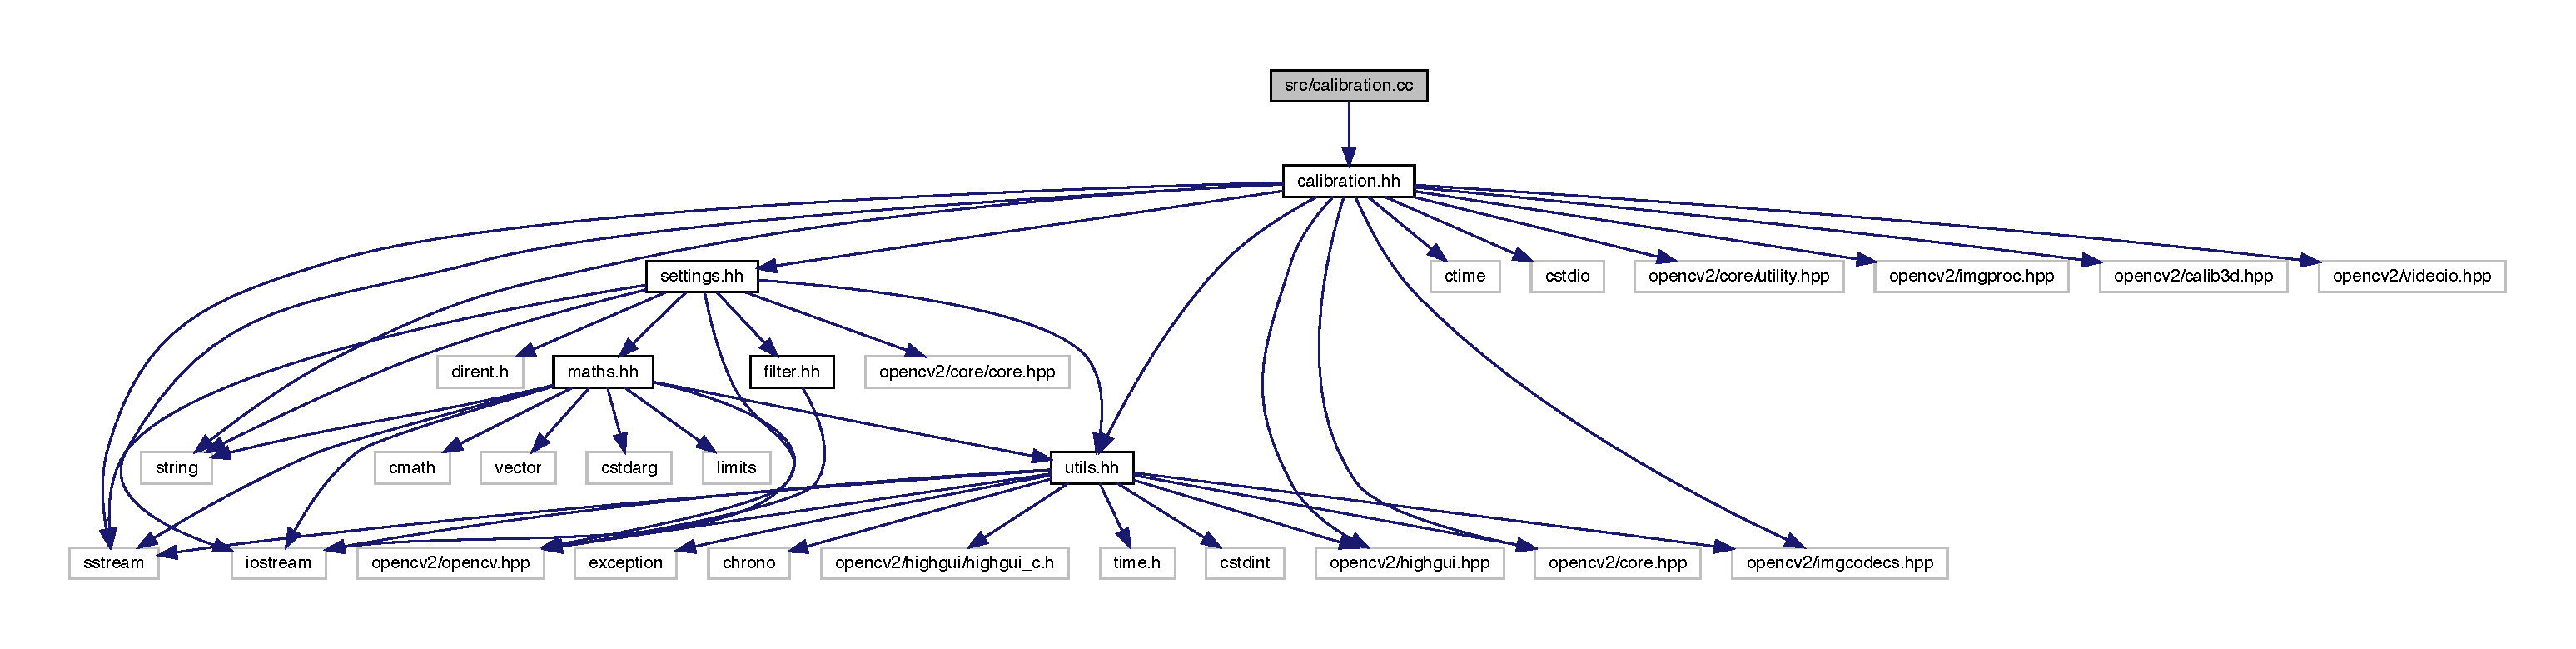
\includegraphics[width=350pt]{calibration_8cc__incl}
\end{center}
\end{figure}
\subsection*{Functions}
\begin{DoxyCompactItemize}
\item 
\mbox{\hyperlink{draw_8hh_aa620a13339ac3a1177c86edc549fda9b}{int}} \mbox{\hyperlink{calibration_8cc_a869b0c5c377f65da8596646d7340d135}{calibration}} (string input\+File)
\begin{DoxyCompactList}\small\item\em Function to run the complete calibration. \end{DoxyCompactList}\item 
static void \mbox{\hyperlink{calibration_8cc_a732d46a8a94e5cc33f89d52dd8395714}{read}} (const File\+Node \&node, \mbox{\hyperlink{class_cal_settings}{Cal\+Settings}} \&x, const \mbox{\hyperlink{class_cal_settings}{Cal\+Settings}} \&default\+\_\+value)
\begin{DoxyCompactList}\small\item\em Reads \mbox{\hyperlink{class_cal_settings}{Cal\+Settings}} from file. If there is none then initiate a new {\ttfamily \mbox{\hyperlink{class_cal_settings}{Cal\+Settings}}}. \end{DoxyCompactList}\item 
static double \mbox{\hyperlink{calibration_8cc_a595849a1b81e38ffd3e1f7f70f88085e}{compute\+Reprojection\+Errors}} (const vector$<$ vector$<$ Point3f $>$ $>$ \&object\+Points, const vector$<$ vector$<$ Point2f $>$ $>$ \&image\+Points, const vector$<$ Mat $>$ \&rvecs, const vector$<$ Mat $>$ \&tvecs, const Mat \&camera\+Matrix, const Mat \&dist\+Coeffs, vector$<$ float $>$ \&per\+View\+Errors, bool fisheye)
\begin{DoxyCompactList}\small\item\em Compute the errors of the projection. \end{DoxyCompactList}\item 
void \mbox{\hyperlink{calibration_8cc_a9deaf00ea7081c5e9ce50a64c9946fa9}{calc\+Board\+Corner\+Positions}} (Size board\+Size, float square\+Size, vector$<$ Point3f $>$ \&corners)
\begin{DoxyCompactList}\small\item\em This function compute the position of the upper corners of every cell. \end{DoxyCompactList}\item 
static bool \mbox{\hyperlink{calibration_8cc_ad985a15627e02f358b321f4d7d47eca1}{run\+Calibration}} (\mbox{\hyperlink{class_cal_settings}{Cal\+Settings}} \&\mbox{\hyperlink{detection_8cc_a9090f9756293390c57567a0bf7630abf}{s}}, Size \&image\+Size, Mat \&camera\+Matrix, Mat \&dist\+Coeffs, vector$<$ vector$<$ Point2f $>$ $>$ image\+Points, vector$<$ Mat $>$ \&rvecs, vector$<$ Mat $>$ \&tvecs, vector$<$ float $>$ \&reproj\+Errs, double \&total\+Avg\+Err)
\begin{DoxyCompactList}\small\item\em This function run the calibration creating the matrixed for the camera and the distorsion coefficients. \end{DoxyCompactList}\item 
static void \mbox{\hyperlink{calibration_8cc_a9a94e87ed45e2dd9c2c5a49b7d01e42f}{save\+Camera\+Params}} (const \mbox{\hyperlink{class_cal_settings}{Cal\+Settings}} \&\mbox{\hyperlink{detection_8cc_a9090f9756293390c57567a0bf7630abf}{s}}, const Size \&image\+Size, const Mat \&camera\+Matrix, const Mat \&dist\+Coeffs, const vector$<$ Mat $>$ \&rvecs, const vector$<$ Mat $>$ \&tvecs, const vector$<$ float $>$ \&reproj\+Errs, const vector$<$ vector$<$ Point2f $>$ $>$ \&image\+Points, const double total\+Avg\+Err)
\begin{DoxyCompactList}\small\item\em Function to save the computed parameters to a file. \end{DoxyCompactList}\item 
bool \mbox{\hyperlink{calibration_8cc_a4195037da024926ac4f645bd09700052}{run\+Calibration\+And\+Save}} (\mbox{\hyperlink{class_cal_settings}{Cal\+Settings}} \&\mbox{\hyperlink{detection_8cc_a9090f9756293390c57567a0bf7630abf}{s}}, Size image\+Size, Mat \&camera\+Matrix, Mat \&dist\+Coeffs, vector$<$ vector$<$ Point2f $>$ $>$ image\+Points)
\begin{DoxyCompactList}\small\item\em Reads \mbox{\hyperlink{class_cal_settings}{Cal\+Settings}} from file. If there is none then initiate a new {\ttfamily \mbox{\hyperlink{class_cal_settings}{Cal\+Settings}}}. \end{DoxyCompactList}\end{DoxyCompactItemize}


\subsection{Function Documentation}
\mbox{\Hypertarget{calibration_8cc_a9deaf00ea7081c5e9ce50a64c9946fa9}\label{calibration_8cc_a9deaf00ea7081c5e9ce50a64c9946fa9}} 
\index{calibration.cc@{calibration.cc}!calcBoardCornerPositions@{calcBoardCornerPositions}}
\index{calcBoardCornerPositions@{calcBoardCornerPositions}!calibration.cc@{calibration.cc}}
\subsubsection{\texorpdfstring{calcBoardCornerPositions()}{calcBoardCornerPositions()}}
{\footnotesize\ttfamily void calc\+Board\+Corner\+Positions (\begin{DoxyParamCaption}\item[{Size}]{board\+Size,  }\item[{float}]{square\+Size,  }\item[{vector$<$ Point3f $>$ \&}]{corners }\end{DoxyParamCaption})}



This function compute the position of the upper corners of every cell. 


\begin{DoxyParams}[1]{Parameters}
\mbox{\texttt{ in}}  & {\em board\+Siz} & The dimension of the chess board. \\
\hline
\mbox{\texttt{ in}}  & {\em square\+Size} & The dimension of the edge of a cell. \\
\hline
\mbox{\texttt{ out}}  & {\em corners} & A vector of Point3fs which equals to the corners of the cells. \\
\hline
\end{DoxyParams}
\mbox{\Hypertarget{calibration_8cc_a869b0c5c377f65da8596646d7340d135}\label{calibration_8cc_a869b0c5c377f65da8596646d7340d135}} 
\index{calibration.cc@{calibration.cc}!calibration@{calibration}}
\index{calibration@{calibration}!calibration.cc@{calibration.cc}}
\subsubsection{\texorpdfstring{calibration()}{calibration()}}
{\footnotesize\ttfamily \mbox{\hyperlink{draw_8hh_aa620a13339ac3a1177c86edc549fda9b}{int}} calibration (\begin{DoxyParamCaption}\item[{string}]{input\+File }\end{DoxyParamCaption})}



Function to run the complete calibration. 


\begin{DoxyParams}[1]{Parameters}
\mbox{\texttt{ in}}  & {\em input\+File} & Name of the setting.\+xml file. It\textquotesingle{}s set to default to default.\+xml\\
\hline
\end{DoxyParams}
\begin{DoxyReturn}{Returns}
-\/2 if the \mbox{\hyperlink{class_cal_settings}{Cal\+Settings}} file could be load but the input was not well-\/formed~\newline
 -\/1 if the \mbox{\hyperlink{class_cal_settings}{Cal\+Settings}} file could not be opened.~\newline
 0 if everything went fine. 
\end{DoxyReturn}
\mbox{\Hypertarget{calibration_8cc_a595849a1b81e38ffd3e1f7f70f88085e}\label{calibration_8cc_a595849a1b81e38ffd3e1f7f70f88085e}} 
\index{calibration.cc@{calibration.cc}!computeReprojectionErrors@{computeReprojectionErrors}}
\index{computeReprojectionErrors@{computeReprojectionErrors}!calibration.cc@{calibration.cc}}
\subsubsection{\texorpdfstring{computeReprojectionErrors()}{computeReprojectionErrors()}}
{\footnotesize\ttfamily static double compute\+Reprojection\+Errors (\begin{DoxyParamCaption}\item[{const vector$<$ vector$<$ Point3f $>$ $>$ \&}]{object\+Points,  }\item[{const vector$<$ vector$<$ Point2f $>$ $>$ \&}]{image\+Points,  }\item[{const vector$<$ Mat $>$ \&}]{rvecs,  }\item[{const vector$<$ Mat $>$ \&}]{tvecs,  }\item[{const Mat \&}]{camera\+Matrix,  }\item[{const Mat \&}]{dist\+Coeffs,  }\item[{vector$<$ float $>$ \&}]{per\+View\+Errors,  }\item[{bool}]{fisheye }\end{DoxyParamCaption})\hspace{0.3cm}{\ttfamily [static]}}



Compute the errors of the projection. 


\begin{DoxyParams}[1]{Parameters}
\mbox{\texttt{ in}}  & {\em object\+Points} & The real image points which will be projected \\
\hline
\mbox{\texttt{ in}}  & {\em rvecs} & Input vector of rotation vectors estimated for each pattern view. \\
\hline
\mbox{\texttt{ in}}  & {\em tvecs} & Input vector of translation vectors estimated for each pattern view. \\
\hline
\mbox{\texttt{ in}}  & {\em camera\+Matrix} & The matrix containing the parameters for the camera \\
\hline
\mbox{\texttt{ in}}  & {\em dist\+Coeffs} & The matrix containing the distortion coefficients. \\
\hline
\mbox{\texttt{ in}}  & {\em fisheye} & A variable which says if a fish eye correction should be applied or no. \\
\hline
\mbox{\texttt{ out}}  & {\em per\+View\+Errors} & A vector containing the error for each image. \\
\hline
\mbox{\texttt{ out}}  & {\em image\+Points} & The projected points for each image.\\
\hline
\end{DoxyParams}
\begin{DoxyReturn}{Returns}
The total error. 
\end{DoxyReturn}
\mbox{\Hypertarget{calibration_8cc_a732d46a8a94e5cc33f89d52dd8395714}\label{calibration_8cc_a732d46a8a94e5cc33f89d52dd8395714}} 
\index{calibration.cc@{calibration.cc}!read@{read}}
\index{read@{read}!calibration.cc@{calibration.cc}}
\subsubsection{\texorpdfstring{read()}{read()}}
{\footnotesize\ttfamily static void read (\begin{DoxyParamCaption}\item[{const File\+Node \&}]{node,  }\item[{\mbox{\hyperlink{class_cal_settings}{Cal\+Settings}} \&}]{x,  }\item[{const \mbox{\hyperlink{class_cal_settings}{Cal\+Settings}} \&}]{default\+\_\+value }\end{DoxyParamCaption})\hspace{0.3cm}{\ttfamily [inline]}, {\ttfamily [static]}}



Reads \mbox{\hyperlink{class_cal_settings}{Cal\+Settings}} from file. If there is none then initiate a new {\ttfamily \mbox{\hyperlink{class_cal_settings}{Cal\+Settings}}}. 


\begin{DoxyParams}[1]{Parameters}
\mbox{\texttt{ in}}  & {\em node} & node to consider for getting \mbox{\hyperlink{class_cal_settings}{Cal\+Settings}}; \\
\hline
\mbox{\texttt{ in}}  & {\em x} & {\ttfamily \mbox{\hyperlink{class_cal_settings}{Cal\+Settings}}} to configure; \\
\hline
\mbox{\texttt{ in}}  & {\em default\+\_\+value} & {\ttfamily \mbox{\hyperlink{class_cal_settings}{Cal\+Settings}}} default value. Setted to {\ttfamily \mbox{\hyperlink{class_cal_settings}{Cal\+Settings()}}}. \\
\hline
\end{DoxyParams}
\mbox{\Hypertarget{calibration_8cc_ad985a15627e02f358b321f4d7d47eca1}\label{calibration_8cc_ad985a15627e02f358b321f4d7d47eca1}} 
\index{calibration.cc@{calibration.cc}!runCalibration@{runCalibration}}
\index{runCalibration@{runCalibration}!calibration.cc@{calibration.cc}}
\subsubsection{\texorpdfstring{runCalibration()}{runCalibration()}}
{\footnotesize\ttfamily static bool run\+Calibration (\begin{DoxyParamCaption}\item[{\mbox{\hyperlink{class_cal_settings}{Cal\+Settings}} \&}]{s,  }\item[{Size \&}]{image\+Size,  }\item[{Mat \&}]{camera\+Matrix,  }\item[{Mat \&}]{dist\+Coeffs,  }\item[{vector$<$ vector$<$ Point2f $>$ $>$}]{image\+Points,  }\item[{vector$<$ Mat $>$ \&}]{rvecs,  }\item[{vector$<$ Mat $>$ \&}]{tvecs,  }\item[{vector$<$ float $>$ \&}]{reproj\+Errs,  }\item[{double \&}]{total\+Avg\+Err }\end{DoxyParamCaption})\hspace{0.3cm}{\ttfamily [static]}}



This function run the calibration creating the matrixed for the camera and the distorsion coefficients. 


\begin{DoxyParams}[1]{Parameters}
\mbox{\texttt{ in}}  & {\em s} & The {\ttfamily \mbox{\hyperlink{class_cal_settings}{Cal\+Settings}}} read from the file and memorized. \\
\hline
\mbox{\texttt{ in}}  & {\em image\+Size} & The size of the image used in {\ttfamily calibrate\+Camera()} to initialize the camera matrix. \\
\hline
\mbox{\texttt{ in}}  & {\em image\+Points} & The projected points for each image. \\
\hline
\mbox{\texttt{ in}}  & {\em reproj\+Errs} & The re-\/projection error, that is a geometric error corresponding to the image distance between a projected point and a measured one. \\
\hline
\mbox{\texttt{ out}}  & {\em camera\+Matrix} & The matrix of the camera parameters \\
\hline
\mbox{\texttt{ out}}  & {\em dist\+Coeffs} & The matrix of the distorsion coefficients. \\
\hline
\mbox{\texttt{ out}}  & {\em rvecs} & Output vector of rotation vectors estimated for each pattern view. \\
\hline
\mbox{\texttt{ out}}  & {\em tvecs} & Output vector of translation vectors estimated for each pattern view. \\
\hline
\mbox{\texttt{ out}}  & {\em total\+Avg\+Err} & The total avarage error given from distorsion.\\
\hline
\end{DoxyParams}
\begin{DoxyReturn}{Returns}
{\ttfamily false} if one or more elements in the {\ttfamily camera\+Matrix} and {\ttfamily dist\+Coeffs} are invalid.~\newline
 {\ttfamily true} if all the elements are valid. 
\end{DoxyReturn}
\mbox{\Hypertarget{calibration_8cc_a4195037da024926ac4f645bd09700052}\label{calibration_8cc_a4195037da024926ac4f645bd09700052}} 
\index{calibration.cc@{calibration.cc}!runCalibrationAndSave@{runCalibrationAndSave}}
\index{runCalibrationAndSave@{runCalibrationAndSave}!calibration.cc@{calibration.cc}}
\subsubsection{\texorpdfstring{runCalibrationAndSave()}{runCalibrationAndSave()}}
{\footnotesize\ttfamily bool run\+Calibration\+And\+Save (\begin{DoxyParamCaption}\item[{\mbox{\hyperlink{class_cal_settings}{Cal\+Settings}} \&}]{s,  }\item[{Size}]{image\+Size,  }\item[{Mat \&}]{camera\+Matrix,  }\item[{Mat \&}]{dist\+Coeffs,  }\item[{vector$<$ vector$<$ Point2f $>$ $>$}]{image\+Points }\end{DoxyParamCaption})}



Reads \mbox{\hyperlink{class_cal_settings}{Cal\+Settings}} from file. If there is none then initiate a new {\ttfamily \mbox{\hyperlink{class_cal_settings}{Cal\+Settings}}}. 


\begin{DoxyParams}[1]{Parameters}
\mbox{\texttt{ in}}  & {\em s} & The {\ttfamily \mbox{\hyperlink{class_cal_settings}{Cal\+Settings}}} being used during the execution. \\
\hline
\mbox{\texttt{ in}}  & {\em image\+Size} & The dimensions of the images. \\
\hline
\mbox{\texttt{ in}}  & {\em image\+Points} & The projected points for each image. \\
\hline
\mbox{\texttt{ out}}  & {\em camera\+Matrix} & The matrix which is used to store the values for the camera parameters. \\
\hline
\mbox{\texttt{ out}}  & {\em dist\+Coeffs} & The matrix which is used to store the distortion coefficients.\\
\hline
\end{DoxyParams}
\begin{DoxyReturn}{Returns}
{\ttfamily true} if the calibration succeded.~\newline
 {\ttfamily false} otherwise. 
\end{DoxyReturn}
\mbox{\Hypertarget{calibration_8cc_a9a94e87ed45e2dd9c2c5a49b7d01e42f}\label{calibration_8cc_a9a94e87ed45e2dd9c2c5a49b7d01e42f}} 
\index{calibration.cc@{calibration.cc}!saveCameraParams@{saveCameraParams}}
\index{saveCameraParams@{saveCameraParams}!calibration.cc@{calibration.cc}}
\subsubsection{\texorpdfstring{saveCameraParams()}{saveCameraParams()}}
{\footnotesize\ttfamily static void save\+Camera\+Params (\begin{DoxyParamCaption}\item[{const \mbox{\hyperlink{class_cal_settings}{Cal\+Settings}} \&}]{s,  }\item[{const Size \&}]{image\+Size,  }\item[{const Mat \&}]{camera\+Matrix,  }\item[{const Mat \&}]{dist\+Coeffs,  }\item[{const vector$<$ Mat $>$ \&}]{rvecs,  }\item[{const vector$<$ Mat $>$ \&}]{tvecs,  }\item[{const vector$<$ float $>$ \&}]{reproj\+Errs,  }\item[{const vector$<$ vector$<$ Point2f $>$ $>$ \&}]{image\+Points,  }\item[{const double}]{total\+Avg\+Err }\end{DoxyParamCaption})\hspace{0.3cm}{\ttfamily [static]}}



Function to save the computed parameters to a file. 


\begin{DoxyParams}[1]{Parameters}
\mbox{\texttt{ in}}  & {\em s} & Use the {\ttfamily \mbox{\hyperlink{class_cal_settings}{Cal\+Settings}}} got at the beginning for information as the output file name, image and board size. \\
\hline
\mbox{\texttt{ in}}  & {\em image\+Size} & The size of the imgage. \\
\hline
\mbox{\texttt{ in}}  & {\em camera\+Matrix} & The camera matrix. \\
\hline
\mbox{\texttt{ in}}  & {\em dist\+Coeffs} & The distorsion coefficient matrix. \\
\hline
 & {\em \mbox{[}int\mbox{]}} & rvecs Vector of rotation vectors estimated for each pattern view. \\
\hline
\mbox{\texttt{ in}}  & {\em tvecs} & Vector of translation vectors estimated for each pattern view. \\
\hline
\mbox{\texttt{ in}}  & {\em reproj\+Errs} & The re-\/projection error, that is a geometric error corresponding to the image distance between a projected point and a measured one. \\
\hline
\mbox{\texttt{ in}}  & {\em image\+Points} & The projected points for each image. \\
\hline
\mbox{\texttt{ in}}  & {\em total\+Avg\+Err} & The total avarage error given from distorsion. \\
\hline
\end{DoxyParams}
Open file for writing

Stores time of calibration

Store infos about the images 
\hypertarget{calibration_8hh}{}\section{src/calibration.hh File Reference}
\label{calibration_8hh}\index{src/calibration.\+hh@{src/calibration.\+hh}}


Library for calibration.  


{\ttfamily \#include \char`\"{}utils.\+hh\char`\"{}}\newline
{\ttfamily \#include $<$iostream$>$}\newline
{\ttfamily \#include $<$sstream$>$}\newline
{\ttfamily \#include $<$string$>$}\newline
{\ttfamily \#include $<$ctime$>$}\newline
{\ttfamily \#include $<$cstdio$>$}\newline
{\ttfamily \#include $<$opencv2/core.\+hpp$>$}\newline
{\ttfamily \#include $<$opencv2/core/utility.\+hpp$>$}\newline
{\ttfamily \#include $<$opencv2/imgproc.\+hpp$>$}\newline
{\ttfamily \#include $<$opencv2/calib3d.\+hpp$>$}\newline
{\ttfamily \#include $<$opencv2/imgcodecs.\+hpp$>$}\newline
{\ttfamily \#include $<$opencv2/videoio.\+hpp$>$}\newline
{\ttfamily \#include $<$opencv2/highgui.\+hpp$>$}\newline
Include dependency graph for calibration.\+hh\+:
\nopagebreak
\begin{figure}[H]
\begin{center}
\leavevmode
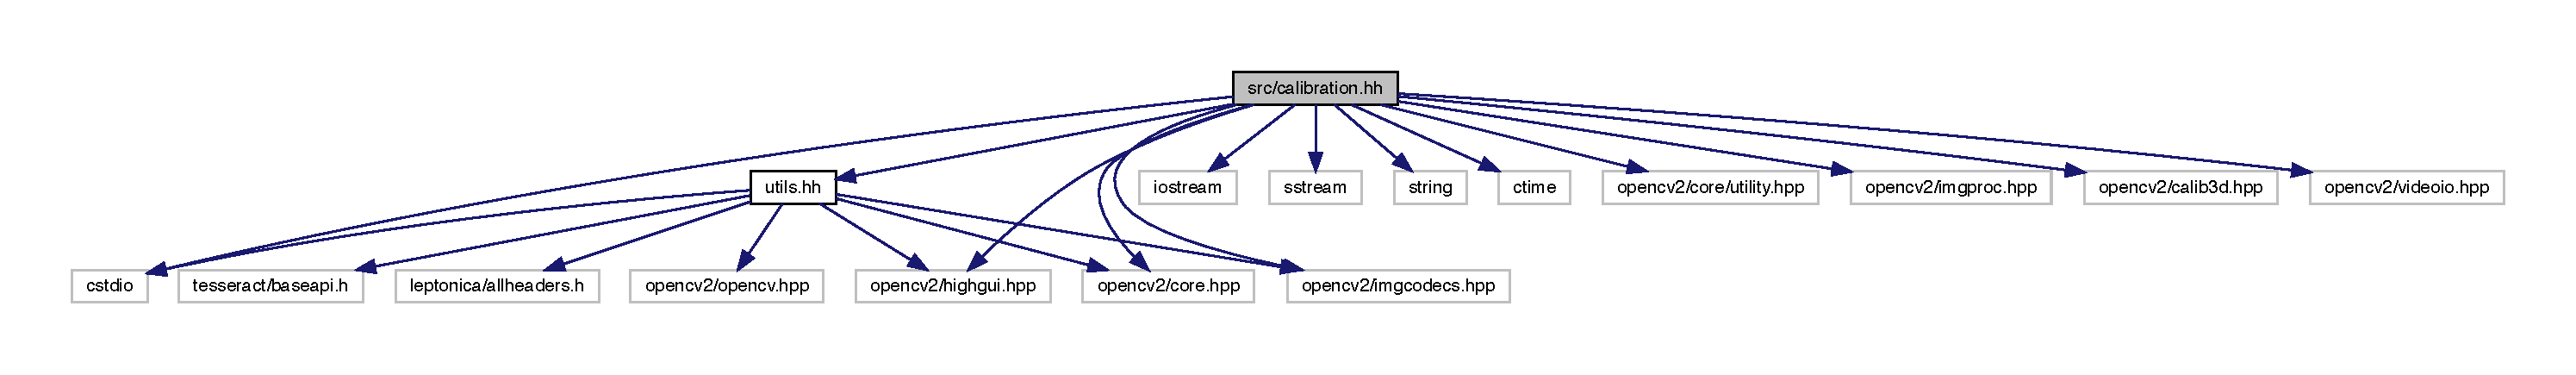
\includegraphics[width=350pt]{calibration_8hh__incl}
\end{center}
\end{figure}
This graph shows which files directly or indirectly include this file\+:
\nopagebreak
\begin{figure}[H]
\begin{center}
\leavevmode
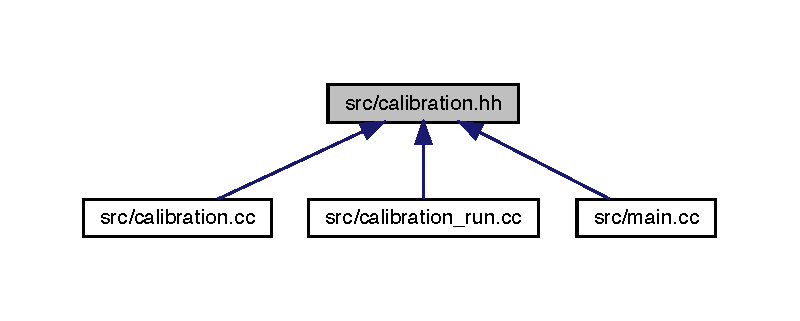
\includegraphics[width=350pt]{calibration_8hh__dep__incl}
\end{center}
\end{figure}
\subsection*{Classes}
\begin{DoxyCompactItemize}
\item 
class \mbox{\hyperlink{class_settings}{Settings}}
\end{DoxyCompactItemize}
\subsection*{Enumerations}
\begin{DoxyCompactItemize}
\item 
enum \{ \mbox{\hyperlink{calibration_8hh_a06fc87d81c62e9abb8790b6e5713c55ba167a7ee1aabe9f27e010fff93c0ba971}{D\+E\+T\+E\+C\+T\+I\+ON}} = 0, 
\mbox{\hyperlink{calibration_8hh_a06fc87d81c62e9abb8790b6e5713c55ba53f5d985011ab26db21516188f46a94f}{C\+A\+P\+T\+U\+R\+I\+NG}} = 1, 
\mbox{\hyperlink{calibration_8hh_a06fc87d81c62e9abb8790b6e5713c55baf7834eaf5a327e180e039aa05dd3ebd1}{C\+A\+L\+I\+B\+R\+A\+T\+ED}} = 2
 \}
\end{DoxyCompactItemize}
\subsection*{Functions}
\begin{DoxyCompactItemize}
\item 
int \mbox{\hyperlink{calibration_8hh_a9deafd96b6adbc102c47af08cde6610c}{calibration}} (const string input\+File=\char`\"{}data/calib\+\_\+config.\+xml\char`\"{})
\begin{DoxyCompactList}\small\item\em Function to run the complete calibration. \end{DoxyCompactList}\item 
bool \mbox{\hyperlink{calibration_8hh_ac7558c8da6af683fc1c86c2ede7bb31c}{run\+Calibration\+And\+Save}} (\mbox{\hyperlink{class_settings}{Settings}} \&s, Size image\+Size, Mat \&camera\+Matrix, Mat \&dist\+Coeffs, vector$<$ vector$<$ Point2f $>$ $>$ image\+Points)
\begin{DoxyCompactList}\small\item\em Reads settings from file. If there is none then initiate a new {\ttfamily \mbox{\hyperlink{class_settings}{Settings}}}. \end{DoxyCompactList}\end{DoxyCompactItemize}


\subsection{Detailed Description}
Library for calibration. 



\subsection{Enumeration Type Documentation}
\mbox{\Hypertarget{calibration_8hh_a06fc87d81c62e9abb8790b6e5713c55b}\label{calibration_8hh_a06fc87d81c62e9abb8790b6e5713c55b}} 
\subsubsection{\texorpdfstring{anonymous enum}{anonymous enum}}
{\footnotesize\ttfamily anonymous enum}

\begin{DoxyEnumFields}{Enumerator}
\raisebox{\heightof{T}}[0pt][0pt]{\index{D\+E\+T\+E\+C\+T\+I\+ON@{D\+E\+T\+E\+C\+T\+I\+ON}!calibration.\+hh@{calibration.\+hh}}\index{calibration.\+hh@{calibration.\+hh}!D\+E\+T\+E\+C\+T\+I\+ON@{D\+E\+T\+E\+C\+T\+I\+ON}}}\mbox{\Hypertarget{calibration_8hh_a06fc87d81c62e9abb8790b6e5713c55ba167a7ee1aabe9f27e010fff93c0ba971}\label{calibration_8hh_a06fc87d81c62e9abb8790b6e5713c55ba167a7ee1aabe9f27e010fff93c0ba971}} 
D\+E\+T\+E\+C\+T\+I\+ON&\\
\hline

\raisebox{\heightof{T}}[0pt][0pt]{\index{C\+A\+P\+T\+U\+R\+I\+NG@{C\+A\+P\+T\+U\+R\+I\+NG}!calibration.\+hh@{calibration.\+hh}}\index{calibration.\+hh@{calibration.\+hh}!C\+A\+P\+T\+U\+R\+I\+NG@{C\+A\+P\+T\+U\+R\+I\+NG}}}\mbox{\Hypertarget{calibration_8hh_a06fc87d81c62e9abb8790b6e5713c55ba53f5d985011ab26db21516188f46a94f}\label{calibration_8hh_a06fc87d81c62e9abb8790b6e5713c55ba53f5d985011ab26db21516188f46a94f}} 
C\+A\+P\+T\+U\+R\+I\+NG&\\
\hline

\raisebox{\heightof{T}}[0pt][0pt]{\index{C\+A\+L\+I\+B\+R\+A\+T\+ED@{C\+A\+L\+I\+B\+R\+A\+T\+ED}!calibration.\+hh@{calibration.\+hh}}\index{calibration.\+hh@{calibration.\+hh}!C\+A\+L\+I\+B\+R\+A\+T\+ED@{C\+A\+L\+I\+B\+R\+A\+T\+ED}}}\mbox{\Hypertarget{calibration_8hh_a06fc87d81c62e9abb8790b6e5713c55baf7834eaf5a327e180e039aa05dd3ebd1}\label{calibration_8hh_a06fc87d81c62e9abb8790b6e5713c55baf7834eaf5a327e180e039aa05dd3ebd1}} 
C\+A\+L\+I\+B\+R\+A\+T\+ED&\\
\hline

\end{DoxyEnumFields}


\subsection{Function Documentation}
\mbox{\Hypertarget{calibration_8hh_a9deafd96b6adbc102c47af08cde6610c}\label{calibration_8hh_a9deafd96b6adbc102c47af08cde6610c}} 
\index{calibration.\+hh@{calibration.\+hh}!calibration@{calibration}}
\index{calibration@{calibration}!calibration.\+hh@{calibration.\+hh}}
\subsubsection{\texorpdfstring{calibration()}{calibration()}}
{\footnotesize\ttfamily int calibration (\begin{DoxyParamCaption}\item[{const string}]{input\+File }\end{DoxyParamCaption})}



Function to run the complete calibration. 


\begin{DoxyParams}[1]{Parameters}
\mbox{\tt in}  & {\em input\+File} & Name of the setting.\+xml file. It\textquotesingle{}s set to default to default.\+xml\\
\hline
\end{DoxyParams}
\begin{DoxyReturn}{Returns}
-\/2 if the settings file could be load but the input was not well-\/formed~\newline
 -\/1 if the settings file could not be opened.~\newline
 0 if everything went fine. 
\end{DoxyReturn}
\mbox{\Hypertarget{calibration_8hh_ac7558c8da6af683fc1c86c2ede7bb31c}\label{calibration_8hh_ac7558c8da6af683fc1c86c2ede7bb31c}} 
\index{calibration.\+hh@{calibration.\+hh}!run\+Calibration\+And\+Save@{run\+Calibration\+And\+Save}}
\index{run\+Calibration\+And\+Save@{run\+Calibration\+And\+Save}!calibration.\+hh@{calibration.\+hh}}
\subsubsection{\texorpdfstring{run\+Calibration\+And\+Save()}{runCalibrationAndSave()}}
{\footnotesize\ttfamily bool run\+Calibration\+And\+Save (\begin{DoxyParamCaption}\item[{\mbox{\hyperlink{class_settings}{Settings}} \&}]{s,  }\item[{Size}]{image\+Size,  }\item[{Mat \&}]{camera\+Matrix,  }\item[{Mat \&}]{dist\+Coeffs,  }\item[{vector$<$ vector$<$ Point2f $>$ $>$}]{image\+Points }\end{DoxyParamCaption})}



Reads settings from file. If there is none then initiate a new {\ttfamily \mbox{\hyperlink{class_settings}{Settings}}}. 


\begin{DoxyParams}[1]{Parameters}
\mbox{\tt in}  & {\em s} & The {\ttfamily \mbox{\hyperlink{class_settings}{Settings}}} being used during the execution. \\
\hline
\mbox{\tt in}  & {\em image\+Size} & The dimensions of the images. \\
\hline
\mbox{\tt in}  & {\em image\+Points} & The projected points for each image. \\
\hline
\mbox{\tt out}  & {\em camera\+Matrix} & The matrix which is used to store the values for the camera parameters. \\
\hline
\mbox{\tt out}  & {\em dist\+Coeffs} & The matrix which is used to store the distortion coefficients.\\
\hline
\end{DoxyParams}
\begin{DoxyReturn}{Returns}
{\ttfamily true} if the calibration succeded.~\newline
 {\ttfamily false} otherwise. 
\end{DoxyReturn}

\hypertarget{calibration__run_8cc}{}\section{src/calibration\+\_\+run.cc File Reference}
\label{calibration__run_8cc}\index{src/calibration\+\_\+run.\+cc@{src/calibration\+\_\+run.\+cc}}
{\ttfamily \#include \char`\"{}calibration.\+hh\char`\"{}}\newline
Include dependency graph for calibration\+\_\+run.\+cc\+:
\nopagebreak
\begin{figure}[H]
\begin{center}
\leavevmode
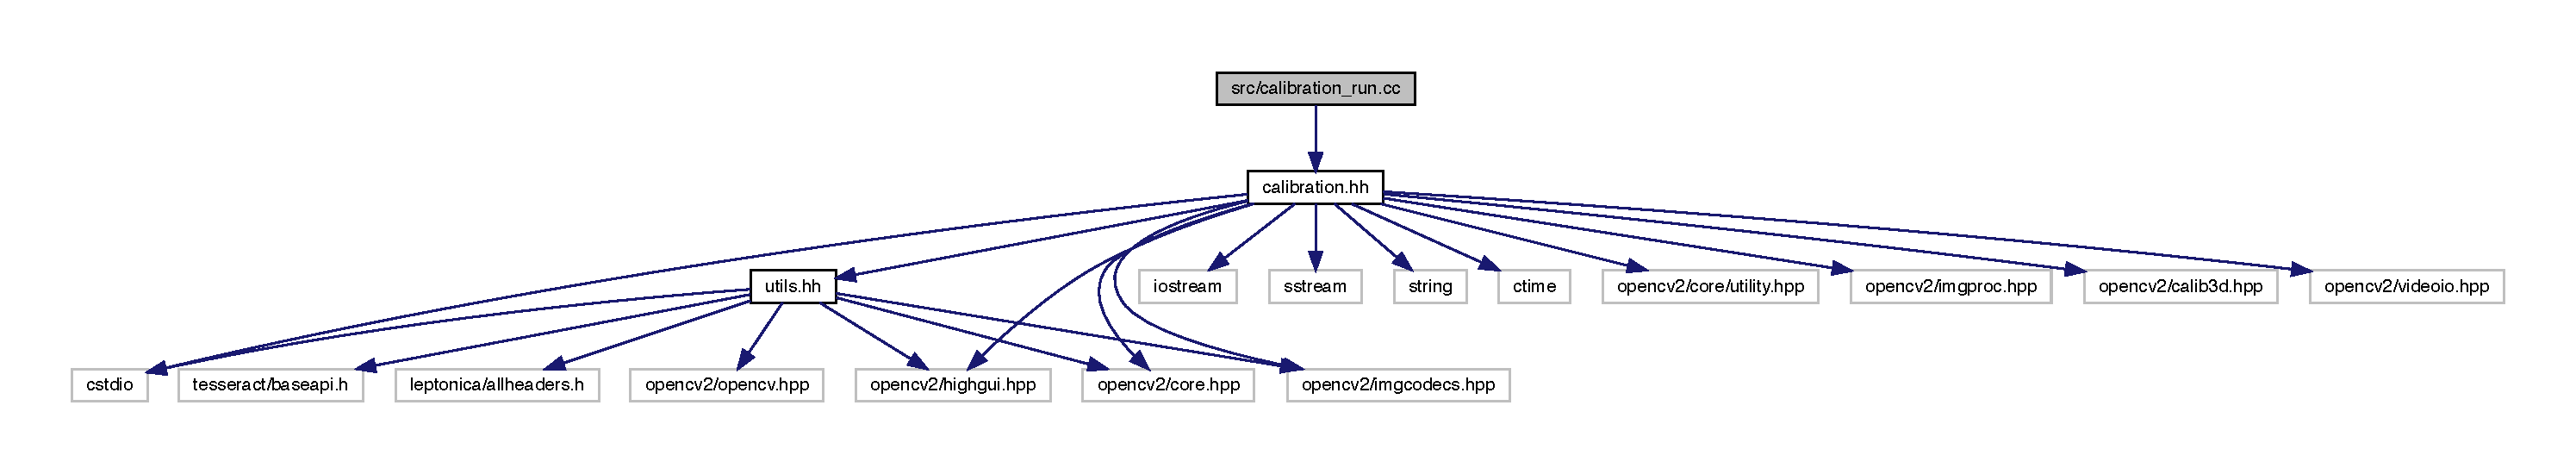
\includegraphics[width=350pt]{calibration__run_8cc__incl}
\end{center}
\end{figure}
\subsection*{Functions}
\begin{DoxyCompactItemize}
\item 
int \mbox{\hyperlink{calibration__run_8cc_ae66f6b31b5ad750f1fe042a706a4e3d4}{main}} ()
\end{DoxyCompactItemize}


\subsection{Function Documentation}
\mbox{\Hypertarget{calibration__run_8cc_ae66f6b31b5ad750f1fe042a706a4e3d4}\label{calibration__run_8cc_ae66f6b31b5ad750f1fe042a706a4e3d4}} 
\index{calibration\+\_\+run.\+cc@{calibration\+\_\+run.\+cc}!main@{main}}
\index{main@{main}!calibration\+\_\+run.\+cc@{calibration\+\_\+run.\+cc}}
\subsubsection{\texorpdfstring{main()}{main()}}
{\footnotesize\ttfamily int main (\begin{DoxyParamCaption}{ }\end{DoxyParamCaption})}


\hypertarget{create__xml_8cc}{}\section{src/create\+\_\+xml.cc File Reference}
\label{create__xml_8cc}\index{src/create\+\_\+xml.\+cc@{src/create\+\_\+xml.\+cc}}
{\ttfamily \#include $<$opencv2/core/core.\+hpp$>$}\newline
{\ttfamily \#include $<$iostream$>$}\newline
{\ttfamily \#include $<$string$>$}\newline
Include dependency graph for create\+\_\+xml.\+cc\+:
\nopagebreak
\begin{figure}[H]
\begin{center}
\leavevmode
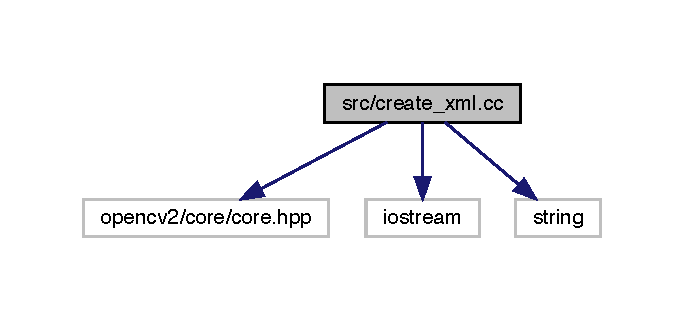
\includegraphics[width=328pt]{create__xml_8cc__incl}
\end{center}
\end{figure}
\subsection*{Functions}
\begin{DoxyCompactItemize}
\item 
int \mbox{\hyperlink{create__xml_8cc_ae66f6b31b5ad750f1fe042a706a4e3d4}{main}} ()
\end{DoxyCompactItemize}


\subsection{Function Documentation}
\mbox{\Hypertarget{create__xml_8cc_ae66f6b31b5ad750f1fe042a706a4e3d4}\label{create__xml_8cc_ae66f6b31b5ad750f1fe042a706a4e3d4}} 
\index{create\+\_\+xml.\+cc@{create\+\_\+xml.\+cc}!main@{main}}
\index{main@{main}!create\+\_\+xml.\+cc@{create\+\_\+xml.\+cc}}
\subsubsection{\texorpdfstring{main()}{main()}}
{\footnotesize\ttfamily int main (\begin{DoxyParamCaption}{ }\end{DoxyParamCaption})}


\hypertarget{detection_8cc}{}\section{src/detection.cc File Reference}
\label{detection_8cc}\index{src/detection.cc@{src/detection.cc}}
{\ttfamily \#include \char`\"{}detection.\+hh\char`\"{}}\newline
Include dependency graph for detection.\+cc\+:
\nopagebreak
\begin{figure}[H]
\begin{center}
\leavevmode
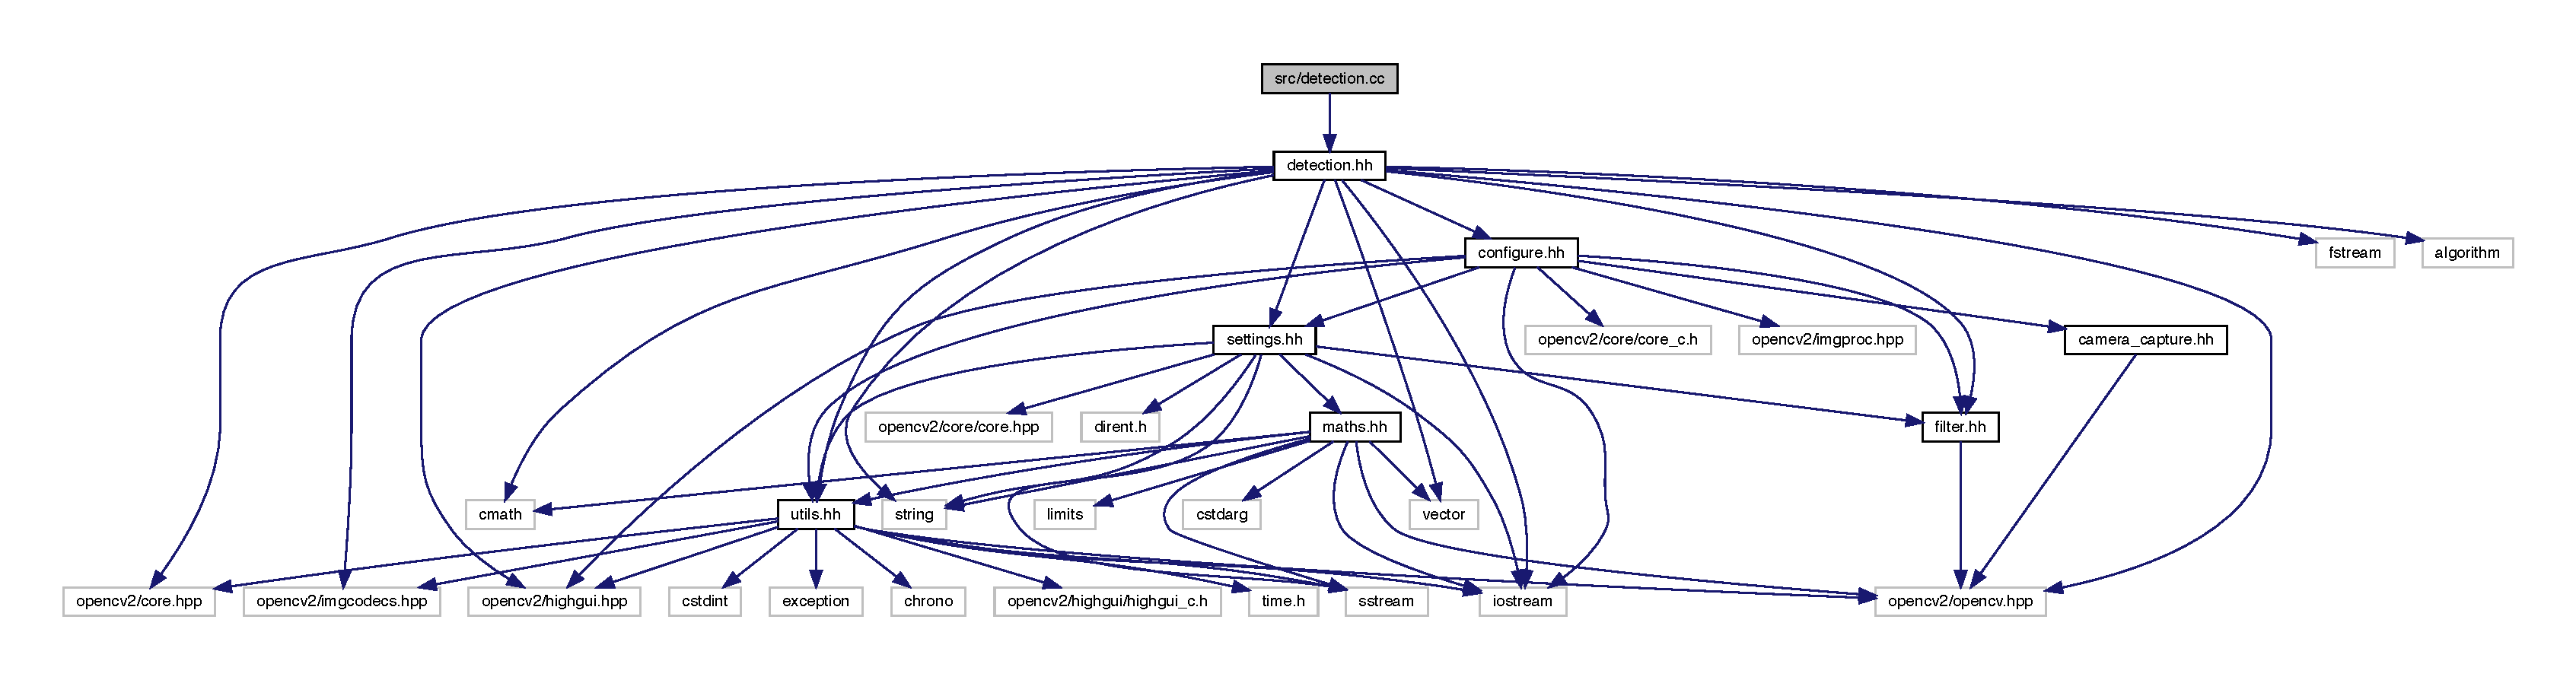
\includegraphics[width=350pt]{detection_8cc__incl}
\end{center}
\end{figure}
\subsection*{Macros}
\begin{DoxyCompactItemize}
\item 
\#define \mbox{\hyperlink{detection_8cc_a0cfe53ea953c48d0949ffb63574ccd3b}{E\+P\+S\+\_\+\+C\+U\+R\+VE}}~3
\begin{DoxyCompactList}\small\item\em Given an image, in black/white format, identify all the borders that delimit the shapes. \end{DoxyCompactList}\end{DoxyCompactItemize}
\subsection*{Functions}
\begin{DoxyCompactItemize}
\item 
\mbox{\hyperlink{draw_8hh_aa620a13339ac3a1177c86edc549fda9b}{int}} \mbox{\hyperlink{detection_8cc_a17e13c447692201697b084a1906cf6fb}{detection}} ()
\begin{DoxyCompactList}\small\item\em Loads some images and detects shapes according to different colors. \end{DoxyCompactList}\item 
void \mbox{\hyperlink{detection_8cc_a50993b0aa4f01d89a4e5d0aef4e1e5f4}{load\+\_\+number\+\_\+template}} ()
\begin{DoxyCompactList}\small\item\em Load some templates and save them in the global variable \textquotesingle{}templates\textquotesingle{}. \end{DoxyCompactList}\item 
void \mbox{\hyperlink{detection_8cc_ac47563337453ac7d1314fe83218c87fc}{shape\+\_\+detection}} (const Mat \&img, const \mbox{\hyperlink{draw_8hh_aa620a13339ac3a1177c86edc549fda9b}{int}} color, const Mat \&un\+\_\+img)
\begin{DoxyCompactList}\small\item\em Detect shapes inside the image according to the variable \textquotesingle{}color\textquotesingle{}. \end{DoxyCompactList}\item 
void \mbox{\hyperlink{detection_8cc_a28d0cdb56cfb2164f939dc2f83d1d9d0}{erode\+\_\+dilation}} (Mat \&img, const \mbox{\hyperlink{draw_8hh_aa620a13339ac3a1177c86edc549fda9b}{int}} color)
\begin{DoxyCompactList}\small\item\em It apply some filtering function for isolate the subject and remove the noise. \end{DoxyCompactList}\item 
void \mbox{\hyperlink{detection_8cc_a93844a9ac3d8be0bd871bb41f8260330}{find\+\_\+contours}} (const Mat \&img, Mat original, const \mbox{\hyperlink{draw_8hh_aa620a13339ac3a1177c86edc549fda9b}{int}} color)
\begin{DoxyCompactList}\small\item\em Given an image, in black/white format, identify all the borders that delimit the shapes. \end{DoxyCompactList}\item 
void \mbox{\hyperlink{detection_8cc_a923b178671e2272c6b082335d118716a}{save\+\_\+convex\+\_\+hull}} (const vector$<$ vector$<$ Point $>$$>$ \&contours, const \mbox{\hyperlink{draw_8hh_aa620a13339ac3a1177c86edc549fda9b}{int}} color, const vector$<$ \mbox{\hyperlink{draw_8hh_aa620a13339ac3a1177c86edc549fda9b}{int}} $>$ \&victims)
\begin{DoxyCompactList}\small\item\em Given some vector save it in a xml file. \end{DoxyCompactList}\item 
\mbox{\hyperlink{draw_8hh_aa620a13339ac3a1177c86edc549fda9b}{int}} \mbox{\hyperlink{detection_8cc_a785fcf35ca81d113a1ea3d831fbdbc22}{number\+\_\+recognition}} (Rect blob, const Mat \&base)
\begin{DoxyCompactList}\small\item\em Detect a number on an image inside a region of interest. \end{DoxyCompactList}\item 
void \mbox{\hyperlink{detection_8cc_a2a7fdd973151b59a6b324eaf4f70fdfe}{crop\+\_\+number\+\_\+section}} (Mat \&R\+OI)
\begin{DoxyCompactList}\small\item\em Given an image identify the region of interest(\+R\+O\+I) and crop it out. \end{DoxyCompactList}\end{DoxyCompactItemize}
\subsection*{Variables}
\begin{DoxyCompactItemize}
\item 
vector$<$ Mat $>$ \mbox{\hyperlink{detection_8cc_ad6ec2d6b7fce088fa5e9f335f9a6ed38}{templates}}
\item 
\mbox{\hyperlink{class_settings}{Settings}} $\ast$ \mbox{\hyperlink{detection_8cc_a9090f9756293390c57567a0bf7630abf}{s}} =new \mbox{\hyperlink{class_settings}{Settings}}
\end{DoxyCompactItemize}


\subsection{Macro Definition Documentation}
\mbox{\Hypertarget{detection_8cc_a0cfe53ea953c48d0949ffb63574ccd3b}\label{detection_8cc_a0cfe53ea953c48d0949ffb63574ccd3b}} 
\index{detection.cc@{detection.cc}!EPS\_CURVE@{EPS\_CURVE}}
\index{EPS\_CURVE@{EPS\_CURVE}!detection.cc@{detection.cc}}
\subsubsection{\texorpdfstring{EPS\_CURVE}{EPS\_CURVE}}
{\footnotesize\ttfamily \#define E\+P\+S\+\_\+\+C\+U\+R\+VE~3}



Given an image, in black/white format, identify all the borders that delimit the shapes. 


\begin{DoxyParams}[1]{Parameters}
\mbox{\texttt{ in}}  & {\em img} & Is an image in H\+SV format at the base of the elaboration process. \\
\hline
\mbox{\texttt{ out}}  & {\em original} & Is the original source of \textquotesingle{}img\textquotesingle{}, it is used for showing the detected contours. \\
\hline
\mbox{\texttt{ in}}  & {\em color} & Can has 3 value\+:~\newline
0 -\/$>$ Red~\newline
1 -\/$>$ Green~\newline
2 -\/$>$ Blue~\newline
Is used for decid which procedure apply to the image. \\
\hline
\end{DoxyParams}


\subsection{Function Documentation}
\mbox{\Hypertarget{detection_8cc_a2a7fdd973151b59a6b324eaf4f70fdfe}\label{detection_8cc_a2a7fdd973151b59a6b324eaf4f70fdfe}} 
\index{detection.cc@{detection.cc}!crop\_number\_section@{crop\_number\_section}}
\index{crop\_number\_section@{crop\_number\_section}!detection.cc@{detection.cc}}
\subsubsection{\texorpdfstring{crop\_number\_section()}{crop\_number\_section()}}
{\footnotesize\ttfamily void crop\+\_\+number\+\_\+section (\begin{DoxyParamCaption}\item[{Mat \&}]{R\+OI }\end{DoxyParamCaption})}



Given an image identify the region of interest(\+R\+O\+I) and crop it out. 


\begin{DoxyParams}[1]{Parameters}
\mbox{\texttt{ in,out}}  & {\em R\+OI} & Is the image that the function will going to elaborate. \\
\hline
\end{DoxyParams}
\mbox{\Hypertarget{detection_8cc_a17e13c447692201697b084a1906cf6fb}\label{detection_8cc_a17e13c447692201697b084a1906cf6fb}} 
\index{detection.cc@{detection.cc}!detection@{detection}}
\index{detection@{detection}!detection.cc@{detection.cc}}
\subsubsection{\texorpdfstring{detection()}{detection()}}
{\footnotesize\ttfamily \mbox{\hyperlink{draw_8hh_aa620a13339ac3a1177c86edc549fda9b}{int}} detection (\begin{DoxyParamCaption}{ }\end{DoxyParamCaption})}



Loads some images and detects shapes according to different colors. 

\begin{DoxyReturn}{Returns}
Return 0 if the function reach the end. 
\end{DoxyReturn}
\mbox{\Hypertarget{detection_8cc_a28d0cdb56cfb2164f939dc2f83d1d9d0}\label{detection_8cc_a28d0cdb56cfb2164f939dc2f83d1d9d0}} 
\index{detection.cc@{detection.cc}!erode\_dilation@{erode\_dilation}}
\index{erode\_dilation@{erode\_dilation}!detection.cc@{detection.cc}}
\subsubsection{\texorpdfstring{erode\_dilation()}{erode\_dilation()}}
{\footnotesize\ttfamily void erode\+\_\+dilation (\begin{DoxyParamCaption}\item[{Mat \&}]{img,  }\item[{const \mbox{\hyperlink{draw_8hh_aa620a13339ac3a1177c86edc549fda9b}{int}}}]{color }\end{DoxyParamCaption})}



It apply some filtering function for isolate the subject and remove the noise. 

An example of the sub functions called are\+: Gaussian\+Blur, Erosion, Dilation and Threshold.


\begin{DoxyParams}[1]{Parameters}
\mbox{\texttt{ in,out}}  & {\em img} & Is the image on which the function apply the filtering. \\
\hline
\mbox{\texttt{ in}}  & {\em color} & Can has 4 value\+:~\newline
0 -\/$>$ Red~\newline
1 -\/$>$ Green~\newline
2 -\/$>$ Blue~\newline
3 -\/$>$ Black~\newline
According to the color the filtering functions apply can change in the type and in the order. \\
\hline
\end{DoxyParams}
\mbox{\Hypertarget{detection_8cc_a93844a9ac3d8be0bd871bb41f8260330}\label{detection_8cc_a93844a9ac3d8be0bd871bb41f8260330}} 
\index{detection.cc@{detection.cc}!find\_contours@{find\_contours}}
\index{find\_contours@{find\_contours}!detection.cc@{detection.cc}}
\subsubsection{\texorpdfstring{find\_contours()}{find\_contours()}}
{\footnotesize\ttfamily void find\+\_\+contours (\begin{DoxyParamCaption}\item[{const Mat \&}]{img,  }\item[{Mat}]{original,  }\item[{const \mbox{\hyperlink{draw_8hh_aa620a13339ac3a1177c86edc549fda9b}{int}}}]{color }\end{DoxyParamCaption})}



Given an image, in black/white format, identify all the borders that delimit the shapes. 


\begin{DoxyParams}[1]{Parameters}
\mbox{\texttt{ in}}  & {\em img} & Is an image in H\+SV format at the base of the elaboration process. \\
\hline
\mbox{\texttt{ out}}  & {\em original} & Is the original source of \textquotesingle{}img\textquotesingle{}, it is used for showing the detected contours. \\
\hline
\mbox{\texttt{ in}}  & {\em color} & Can has 3 value\+:~\newline
0 -\/$>$ Red~\newline
1 -\/$>$ Green~\newline
2 -\/$>$ Blue~\newline
Is used for decid which procedure apply to the image. \\
\hline
\end{DoxyParams}
\mbox{\Hypertarget{detection_8cc_a50993b0aa4f01d89a4e5d0aef4e1e5f4}\label{detection_8cc_a50993b0aa4f01d89a4e5d0aef4e1e5f4}} 
\index{detection.cc@{detection.cc}!load\_number\_template@{load\_number\_template}}
\index{load\_number\_template@{load\_number\_template}!detection.cc@{detection.cc}}
\subsubsection{\texorpdfstring{load\_number\_template()}{load\_number\_template()}}
{\footnotesize\ttfamily void load\+\_\+number\+\_\+template (\begin{DoxyParamCaption}{ }\end{DoxyParamCaption})}



Load some templates and save them in the global variable \textquotesingle{}templates\textquotesingle{}. 

\mbox{\Hypertarget{detection_8cc_a785fcf35ca81d113a1ea3d831fbdbc22}\label{detection_8cc_a785fcf35ca81d113a1ea3d831fbdbc22}} 
\index{detection.cc@{detection.cc}!number\_recognition@{number\_recognition}}
\index{number\_recognition@{number\_recognition}!detection.cc@{detection.cc}}
\subsubsection{\texorpdfstring{number\_recognition()}{number\_recognition()}}
{\footnotesize\ttfamily \mbox{\hyperlink{draw_8hh_aa620a13339ac3a1177c86edc549fda9b}{int}} number\+\_\+recognition (\begin{DoxyParamCaption}\item[{Rect}]{blob,  }\item[{const Mat \&}]{base }\end{DoxyParamCaption})}



Detect a number on an image inside a region of interest. 


\begin{DoxyParams}[1]{Parameters}
\mbox{\texttt{ in}}  & {\em blob} & Identify the region of interest inside the image \textquotesingle{}base\textquotesingle{}. \\
\hline
\mbox{\texttt{ in}}  & {\em base} & Is the image where the function will going to search the number.\\
\hline
\end{DoxyParams}
\begin{DoxyReturn}{Returns}
The number recognise, \textquotesingle{}-\/1\textquotesingle{} otherwise. 
\end{DoxyReturn}
\mbox{\Hypertarget{detection_8cc_a923b178671e2272c6b082335d118716a}\label{detection_8cc_a923b178671e2272c6b082335d118716a}} 
\index{detection.cc@{detection.cc}!save\_convex\_hull@{save\_convex\_hull}}
\index{save\_convex\_hull@{save\_convex\_hull}!detection.cc@{detection.cc}}
\subsubsection{\texorpdfstring{save\_convex\_hull()}{save\_convex\_hull()}}
{\footnotesize\ttfamily void save\+\_\+convex\+\_\+hull (\begin{DoxyParamCaption}\item[{const vector$<$ vector$<$ Point $>$$>$ \&}]{contours,  }\item[{const \mbox{\hyperlink{draw_8hh_aa620a13339ac3a1177c86edc549fda9b}{int}}}]{color,  }\item[{const vector$<$ \mbox{\hyperlink{draw_8hh_aa620a13339ac3a1177c86edc549fda9b}{int}} $>$ \&}]{victims }\end{DoxyParamCaption})}



Given some vector save it in a xml file. 


\begin{DoxyParams}[1]{Parameters}
\mbox{\texttt{ in}}  & {\em contours} & Is a vector that is saved in a xml file. \\
\hline
\mbox{\texttt{ in}}  & {\em color} & Is the parameter according to which the function decide if saved (\textquotesingle{}color==1\textquotesingle{}) or not (\textquotesingle{}otherwise\textquotesingle{}) the vector \textquotesingle{}victims\textquotesingle{}. \\
\hline
\mbox{\texttt{ in}}  & {\em victims} & Is a vector that is saved in a xml file. \\
\hline
\end{DoxyParams}
\mbox{\Hypertarget{detection_8cc_ac47563337453ac7d1314fe83218c87fc}\label{detection_8cc_ac47563337453ac7d1314fe83218c87fc}} 
\index{detection.cc@{detection.cc}!shape\_detection@{shape\_detection}}
\index{shape\_detection@{shape\_detection}!detection.cc@{detection.cc}}
\subsubsection{\texorpdfstring{shape\_detection()}{shape\_detection()}}
{\footnotesize\ttfamily void shape\+\_\+detection (\begin{DoxyParamCaption}\item[{const Mat \&}]{img,  }\item[{const \mbox{\hyperlink{draw_8hh_aa620a13339ac3a1177c86edc549fda9b}{int}}}]{color,  }\item[{const Mat \&}]{un\+\_\+img }\end{DoxyParamCaption})}



Detect shapes inside the image according to the variable \textquotesingle{}color\textquotesingle{}. 


\begin{DoxyParams}[1]{Parameters}
\mbox{\texttt{ in}}  & {\em img} & Image on which the research will done. \\
\hline
\mbox{\texttt{ in}}  & {\em color} & Can has 3 value\+:~\newline
0 -\/$>$ Red~\newline
1 -\/$>$ Green~\newline
2 -\/$>$ Blue~\newline
These color identify the possible spectrum that the function search on the image. \\
\hline
\end{DoxyParams}


\subsection{Variable Documentation}
\mbox{\Hypertarget{detection_8cc_a9090f9756293390c57567a0bf7630abf}\label{detection_8cc_a9090f9756293390c57567a0bf7630abf}} 
\index{detection.cc@{detection.cc}!s@{s}}
\index{s@{s}!detection.cc@{detection.cc}}
\subsubsection{\texorpdfstring{s}{s}}
{\footnotesize\ttfamily \mbox{\hyperlink{class_settings}{Settings}}$\ast$ s =new \mbox{\hyperlink{class_settings}{Settings}}}

\mbox{\Hypertarget{detection_8cc_ad6ec2d6b7fce088fa5e9f335f9a6ed38}\label{detection_8cc_ad6ec2d6b7fce088fa5e9f335f9a6ed38}} 
\index{detection.cc@{detection.cc}!templates@{templates}}
\index{templates@{templates}!detection.cc@{detection.cc}}
\subsubsection{\texorpdfstring{templates}{templates}}
{\footnotesize\ttfamily vector$<$Mat$>$ templates}


\hypertarget{detection_8hh}{}\section{src/include/detection.hh File Reference}
\label{detection_8hh}\index{src/include/detection.hh@{src/include/detection.hh}}
{\ttfamily \#include $<$tesseract/baseapi.\+h$>$}\newline
{\ttfamily \#include $<$leptonica/allheaders.\+h$>$}\newline
{\ttfamily \#include $<$utils.\+hh$>$}\newline
{\ttfamily \#include $<$iostream$>$}\newline
{\ttfamily \#include $<$fstream$>$}\newline
{\ttfamily \#include $<$string$>$}\newline
{\ttfamily \#include $<$cmath$>$}\newline
{\ttfamily \#include $<$opencv2/highgui.\+hpp$>$}\newline
{\ttfamily \#include $<$opencv2/core.\+hpp$>$}\newline
{\ttfamily \#include $<$opencv2/opencv.\+hpp$>$}\newline
{\ttfamily \#include $<$opencv2/imgcodecs.\+hpp$>$}\newline
Include dependency graph for detection.\+hh\+:
\nopagebreak
\begin{figure}[H]
\begin{center}
\leavevmode
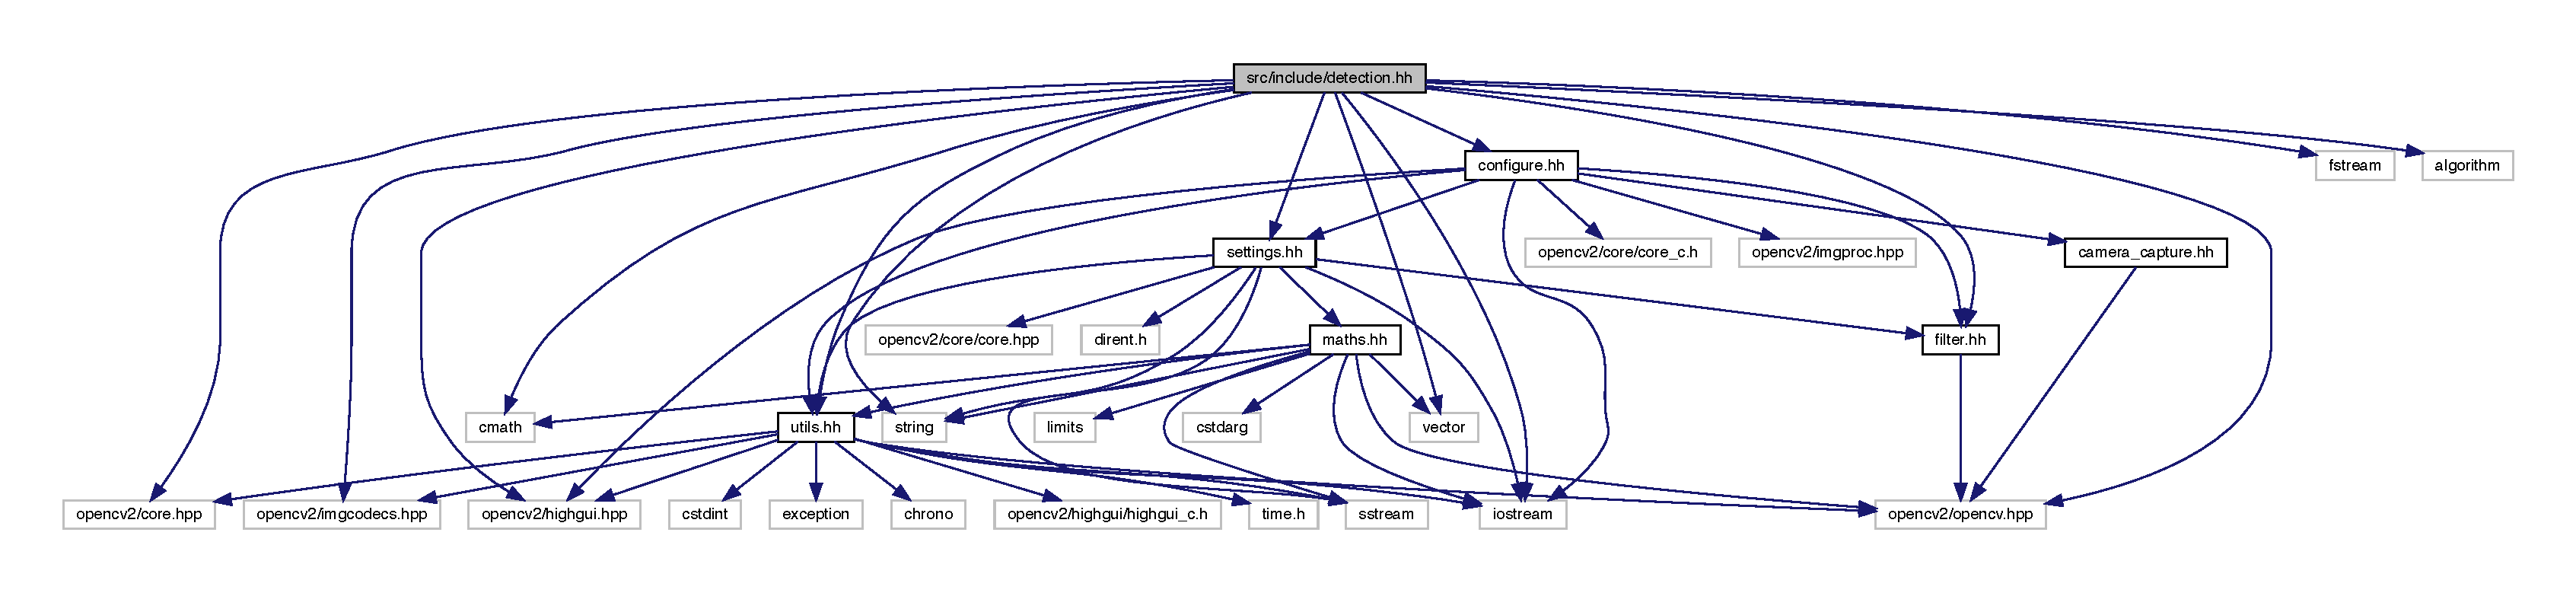
\includegraphics[width=350pt]{detection_8hh__incl}
\end{center}
\end{figure}
This graph shows which files directly or indirectly include this file\+:
\nopagebreak
\begin{figure}[H]
\begin{center}
\leavevmode
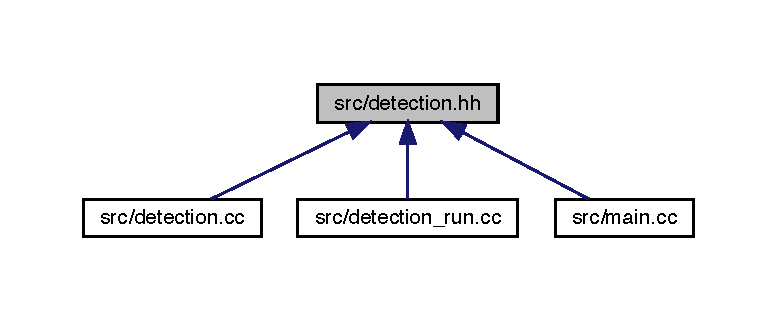
\includegraphics[width=350pt]{detection_8hh__dep__incl}
\end{center}
\end{figure}
\subsection*{Functions}
\begin{DoxyCompactItemize}
\item 
\mbox{\hyperlink{draw_8hh_aa620a13339ac3a1177c86edc549fda9b}{int}} \mbox{\hyperlink{detection_8hh_a17e13c447692201697b084a1906cf6fb}{detection}} ()
\begin{DoxyCompactList}\small\item\em Loads some images and detects shapes according to different colors. \end{DoxyCompactList}\item 
void \mbox{\hyperlink{detection_8hh_ac47563337453ac7d1314fe83218c87fc}{shape\+\_\+detection}} (const Mat \&img, const \mbox{\hyperlink{draw_8hh_aa620a13339ac3a1177c86edc549fda9b}{int}} color, const Mat \&un\+\_\+img)
\begin{DoxyCompactList}\small\item\em Detect shapes inside the image according to the variable \textquotesingle{}color\textquotesingle{}. \end{DoxyCompactList}\item 
void \mbox{\hyperlink{detection_8hh_a28d0cdb56cfb2164f939dc2f83d1d9d0}{erode\+\_\+dilation}} (Mat \&img, const \mbox{\hyperlink{draw_8hh_aa620a13339ac3a1177c86edc549fda9b}{int}} color)
\begin{DoxyCompactList}\small\item\em It apply some filtering function for isolate the subject and remove the noise. \end{DoxyCompactList}\item 
void \mbox{\hyperlink{detection_8hh_a93844a9ac3d8be0bd871bb41f8260330}{find\+\_\+contours}} (const Mat \&img, Mat original, const \mbox{\hyperlink{draw_8hh_aa620a13339ac3a1177c86edc549fda9b}{int}} color)
\begin{DoxyCompactList}\small\item\em Given an image, in black/white format, identify all the borders that delimit the shapes. \end{DoxyCompactList}\item 
\mbox{\hyperlink{draw_8hh_aa620a13339ac3a1177c86edc549fda9b}{int}} \mbox{\hyperlink{detection_8hh_a785fcf35ca81d113a1ea3d831fbdbc22}{number\+\_\+recognition}} (Rect blob, const Mat \&base)
\begin{DoxyCompactList}\small\item\em Detect a number on an image inside a region of interest. \end{DoxyCompactList}\item 
void \mbox{\hyperlink{detection_8hh_a923b178671e2272c6b082335d118716a}{save\+\_\+convex\+\_\+hull}} (const vector$<$ vector$<$ Point $>$$>$ \&contours, const \mbox{\hyperlink{draw_8hh_aa620a13339ac3a1177c86edc549fda9b}{int}} color, const vector$<$ \mbox{\hyperlink{draw_8hh_aa620a13339ac3a1177c86edc549fda9b}{int}} $>$ \&victims)
\begin{DoxyCompactList}\small\item\em Given some vector save it in a xml file. \end{DoxyCompactList}\item 
void \mbox{\hyperlink{detection_8hh_a50993b0aa4f01d89a4e5d0aef4e1e5f4}{load\+\_\+number\+\_\+template}} ()
\begin{DoxyCompactList}\small\item\em Load some templates and save them in the global variable \textquotesingle{}templates\textquotesingle{}. \end{DoxyCompactList}\item 
void \mbox{\hyperlink{detection_8hh_a8edaf0da54add7cd1461bafecef26b56}{crop\+\_\+number\+\_\+section}} (Mat \&process\+R\+OI)
\begin{DoxyCompactList}\small\item\em Given an image identify the region of interest(\+R\+O\+I) and crop it out. \end{DoxyCompactList}\end{DoxyCompactItemize}


\subsection{Function Documentation}
\mbox{\Hypertarget{detection_8hh_a8edaf0da54add7cd1461bafecef26b56}\label{detection_8hh_a8edaf0da54add7cd1461bafecef26b56}} 
\index{detection.hh@{detection.hh}!crop\_number\_section@{crop\_number\_section}}
\index{crop\_number\_section@{crop\_number\_section}!detection.hh@{detection.hh}}
\subsubsection{\texorpdfstring{crop\_number\_section()}{crop\_number\_section()}}
{\footnotesize\ttfamily void crop\+\_\+number\+\_\+section (\begin{DoxyParamCaption}\item[{Mat \&}]{R\+OI }\end{DoxyParamCaption})}



Given an image identify the region of interest(\+R\+O\+I) and crop it out. 


\begin{DoxyParams}[1]{Parameters}
\mbox{\texttt{ in,out}}  & {\em R\+OI} & Is the image that the function will going to elaborate. \\
\hline
\end{DoxyParams}
\mbox{\Hypertarget{detection_8hh_a17e13c447692201697b084a1906cf6fb}\label{detection_8hh_a17e13c447692201697b084a1906cf6fb}} 
\index{detection.hh@{detection.hh}!detection@{detection}}
\index{detection@{detection}!detection.hh@{detection.hh}}
\subsubsection{\texorpdfstring{detection()}{detection()}}
{\footnotesize\ttfamily \mbox{\hyperlink{draw_8hh_aa620a13339ac3a1177c86edc549fda9b}{int}} detection (\begin{DoxyParamCaption}{ }\end{DoxyParamCaption})}



Loads some images and detects shapes according to different colors. 

\begin{DoxyReturn}{Returns}
Return 0 if the function reach the end. 
\end{DoxyReturn}
\mbox{\Hypertarget{detection_8hh_a28d0cdb56cfb2164f939dc2f83d1d9d0}\label{detection_8hh_a28d0cdb56cfb2164f939dc2f83d1d9d0}} 
\index{detection.hh@{detection.hh}!erode\_dilation@{erode\_dilation}}
\index{erode\_dilation@{erode\_dilation}!detection.hh@{detection.hh}}
\subsubsection{\texorpdfstring{erode\_dilation()}{erode\_dilation()}}
{\footnotesize\ttfamily void erode\+\_\+dilation (\begin{DoxyParamCaption}\item[{Mat \&}]{img,  }\item[{const \mbox{\hyperlink{draw_8hh_aa620a13339ac3a1177c86edc549fda9b}{int}}}]{color }\end{DoxyParamCaption})}



It apply some filtering function for isolate the subject and remove the noise. 

An example of the sub functions called are\+: Gaussian\+Blur, Erosion, Dilation and Threshold.


\begin{DoxyParams}[1]{Parameters}
\mbox{\texttt{ in,out}}  & {\em img} & Is the image on which the function apply the filtering. \\
\hline
\mbox{\texttt{ in}}  & {\em color} & Can has 4 value\+:~\newline
0 -\/$>$ Red~\newline
1 -\/$>$ Green~\newline
2 -\/$>$ Blue~\newline
3 -\/$>$ Black~\newline
According to the color the filtering functions apply can change in the type and in the order. \\
\hline
\end{DoxyParams}
\mbox{\Hypertarget{detection_8hh_a93844a9ac3d8be0bd871bb41f8260330}\label{detection_8hh_a93844a9ac3d8be0bd871bb41f8260330}} 
\index{detection.hh@{detection.hh}!find\_contours@{find\_contours}}
\index{find\_contours@{find\_contours}!detection.hh@{detection.hh}}
\subsubsection{\texorpdfstring{find\_contours()}{find\_contours()}}
{\footnotesize\ttfamily void find\+\_\+contours (\begin{DoxyParamCaption}\item[{const Mat \&}]{img,  }\item[{Mat}]{original,  }\item[{const \mbox{\hyperlink{draw_8hh_aa620a13339ac3a1177c86edc549fda9b}{int}}}]{color }\end{DoxyParamCaption})}



Given an image, in black/white format, identify all the borders that delimit the shapes. 


\begin{DoxyParams}[1]{Parameters}
\mbox{\texttt{ in}}  & {\em img} & Is an image in H\+SV format at the base of the elaboration process. \\
\hline
\mbox{\texttt{ out}}  & {\em original} & Is the original source of \textquotesingle{}img\textquotesingle{}, it is used for showing the detected contours. \\
\hline
\mbox{\texttt{ in}}  & {\em color} & Can has 3 value\+:~\newline
0 -\/$>$ Red~\newline
1 -\/$>$ Green~\newline
2 -\/$>$ Blue~\newline
Is used for decid which procedure apply to the image. \\
\hline
\end{DoxyParams}
\mbox{\Hypertarget{detection_8hh_a50993b0aa4f01d89a4e5d0aef4e1e5f4}\label{detection_8hh_a50993b0aa4f01d89a4e5d0aef4e1e5f4}} 
\index{detection.hh@{detection.hh}!load\_number\_template@{load\_number\_template}}
\index{load\_number\_template@{load\_number\_template}!detection.hh@{detection.hh}}
\subsubsection{\texorpdfstring{load\_number\_template()}{load\_number\_template()}}
{\footnotesize\ttfamily void load\+\_\+number\+\_\+template (\begin{DoxyParamCaption}{ }\end{DoxyParamCaption})}



Load some templates and save them in the global variable \textquotesingle{}templates\textquotesingle{}. 

\mbox{\Hypertarget{detection_8hh_a785fcf35ca81d113a1ea3d831fbdbc22}\label{detection_8hh_a785fcf35ca81d113a1ea3d831fbdbc22}} 
\index{detection.hh@{detection.hh}!number\_recognition@{number\_recognition}}
\index{number\_recognition@{number\_recognition}!detection.hh@{detection.hh}}
\subsubsection{\texorpdfstring{number\_recognition()}{number\_recognition()}}
{\footnotesize\ttfamily \mbox{\hyperlink{draw_8hh_aa620a13339ac3a1177c86edc549fda9b}{int}} number\+\_\+recognition (\begin{DoxyParamCaption}\item[{Rect}]{blob,  }\item[{const Mat \&}]{base }\end{DoxyParamCaption})}



Detect a number on an image inside a region of interest. 


\begin{DoxyParams}[1]{Parameters}
\mbox{\texttt{ in}}  & {\em blob} & Identify the region of interest inside the image \textquotesingle{}base\textquotesingle{}. \\
\hline
\mbox{\texttt{ in}}  & {\em base} & Is the image where the function will going to search the number.\\
\hline
\end{DoxyParams}
\begin{DoxyReturn}{Returns}
The number recognise, \textquotesingle{}-\/1\textquotesingle{} otherwise. 
\end{DoxyReturn}
\mbox{\Hypertarget{detection_8hh_a923b178671e2272c6b082335d118716a}\label{detection_8hh_a923b178671e2272c6b082335d118716a}} 
\index{detection.hh@{detection.hh}!save\_convex\_hull@{save\_convex\_hull}}
\index{save\_convex\_hull@{save\_convex\_hull}!detection.hh@{detection.hh}}
\subsubsection{\texorpdfstring{save\_convex\_hull()}{save\_convex\_hull()}}
{\footnotesize\ttfamily void save\+\_\+convex\+\_\+hull (\begin{DoxyParamCaption}\item[{const vector$<$ vector$<$ Point $>$$>$ \&}]{contours,  }\item[{const \mbox{\hyperlink{draw_8hh_aa620a13339ac3a1177c86edc549fda9b}{int}}}]{color,  }\item[{const vector$<$ \mbox{\hyperlink{draw_8hh_aa620a13339ac3a1177c86edc549fda9b}{int}} $>$ \&}]{victims }\end{DoxyParamCaption})}



Given some vector save it in a xml file. 


\begin{DoxyParams}[1]{Parameters}
\mbox{\texttt{ in}}  & {\em contours} & Is a vector that is saved in a xml file. \\
\hline
\mbox{\texttt{ in}}  & {\em color} & Is the parameter according to which the function decide if saved (\textquotesingle{}color==1\textquotesingle{}) or not (\textquotesingle{}otherwise\textquotesingle{}) the vector \textquotesingle{}victims\textquotesingle{}. \\
\hline
\mbox{\texttt{ in}}  & {\em victims} & Is a vector that is saved in a xml file. \\
\hline
\end{DoxyParams}
\mbox{\Hypertarget{detection_8hh_ac47563337453ac7d1314fe83218c87fc}\label{detection_8hh_ac47563337453ac7d1314fe83218c87fc}} 
\index{detection.hh@{detection.hh}!shape\_detection@{shape\_detection}}
\index{shape\_detection@{shape\_detection}!detection.hh@{detection.hh}}
\subsubsection{\texorpdfstring{shape\_detection()}{shape\_detection()}}
{\footnotesize\ttfamily void shape\+\_\+detection (\begin{DoxyParamCaption}\item[{const Mat \&}]{img,  }\item[{const \mbox{\hyperlink{draw_8hh_aa620a13339ac3a1177c86edc549fda9b}{int}}}]{color,  }\item[{const Mat \&}]{un\+\_\+img }\end{DoxyParamCaption})}



Detect shapes inside the image according to the variable \textquotesingle{}color\textquotesingle{}. 


\begin{DoxyParams}[1]{Parameters}
\mbox{\texttt{ in}}  & {\em img} & Image on which the research will done. \\
\hline
\mbox{\texttt{ in}}  & {\em color} & Can has 3 value\+:~\newline
0 -\/$>$ Red~\newline
1 -\/$>$ Green~\newline
2 -\/$>$ Blue~\newline
These color identify the possible spectrum that the function search on the image. \\
\hline
\end{DoxyParams}

\hypertarget{detection__run_8cc}{}\section{src/run/detection\+\_\+run.cc File Reference}
\label{detection__run_8cc}\index{src/run/detection\_run.cc@{src/run/detection\_run.cc}}
{\ttfamily \#include $<$detection.\+hh$>$}\newline
Include dependency graph for detection\+\_\+run.\+cc\+:
\nopagebreak
\begin{figure}[H]
\begin{center}
\leavevmode
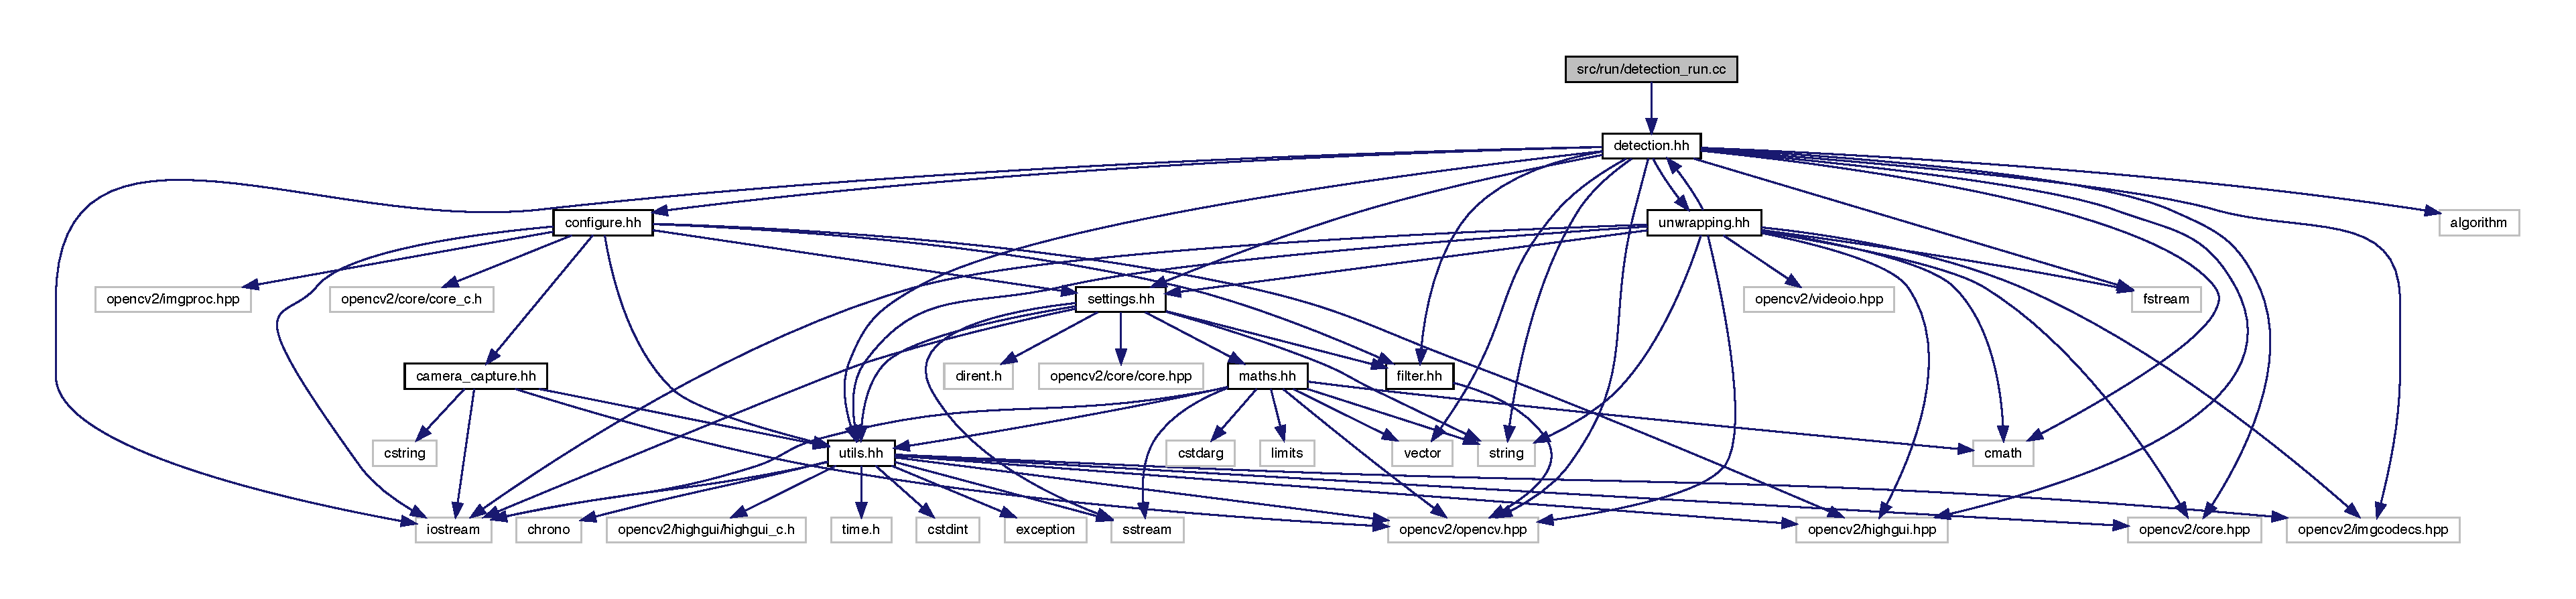
\includegraphics[width=350pt]{detection__run_8cc__incl}
\end{center}
\end{figure}
\subsection*{Functions}
\begin{DoxyCompactItemize}
\item 
\mbox{\hyperlink{draw_8hh_aa620a13339ac3a1177c86edc549fda9b}{int}} \mbox{\hyperlink{detection__run_8cc_ae66f6b31b5ad750f1fe042a706a4e3d4}{main}} ()
\end{DoxyCompactItemize}


\subsection{Function Documentation}
\mbox{\Hypertarget{detection__run_8cc_ae66f6b31b5ad750f1fe042a706a4e3d4}\label{detection__run_8cc_ae66f6b31b5ad750f1fe042a706a4e3d4}} 
\index{detection\_run.cc@{detection\_run.cc}!main@{main}}
\index{main@{main}!detection\_run.cc@{detection\_run.cc}}
\subsubsection{\texorpdfstring{main()}{main()}}
{\footnotesize\ttfamily \mbox{\hyperlink{draw_8hh_aa620a13339ac3a1177c86edc549fda9b}{int}} main (\begin{DoxyParamCaption}{ }\end{DoxyParamCaption})}


\hypertarget{main_8cc}{}\section{src/run/main.cc File Reference}
\label{main_8cc}\index{src/run/main.cc@{src/run/main.cc}}
{\ttfamily \#include $<$detection.\+hh$>$}\newline
{\ttfamily \#include $<$unwrapping.\+hh$>$}\newline
{\ttfamily \#include $<$configure.\+hh$>$}\newline
{\ttfamily \#include $<$iostream$>$}\newline
Include dependency graph for main.\+cc\+:
\nopagebreak
\begin{figure}[H]
\begin{center}
\leavevmode
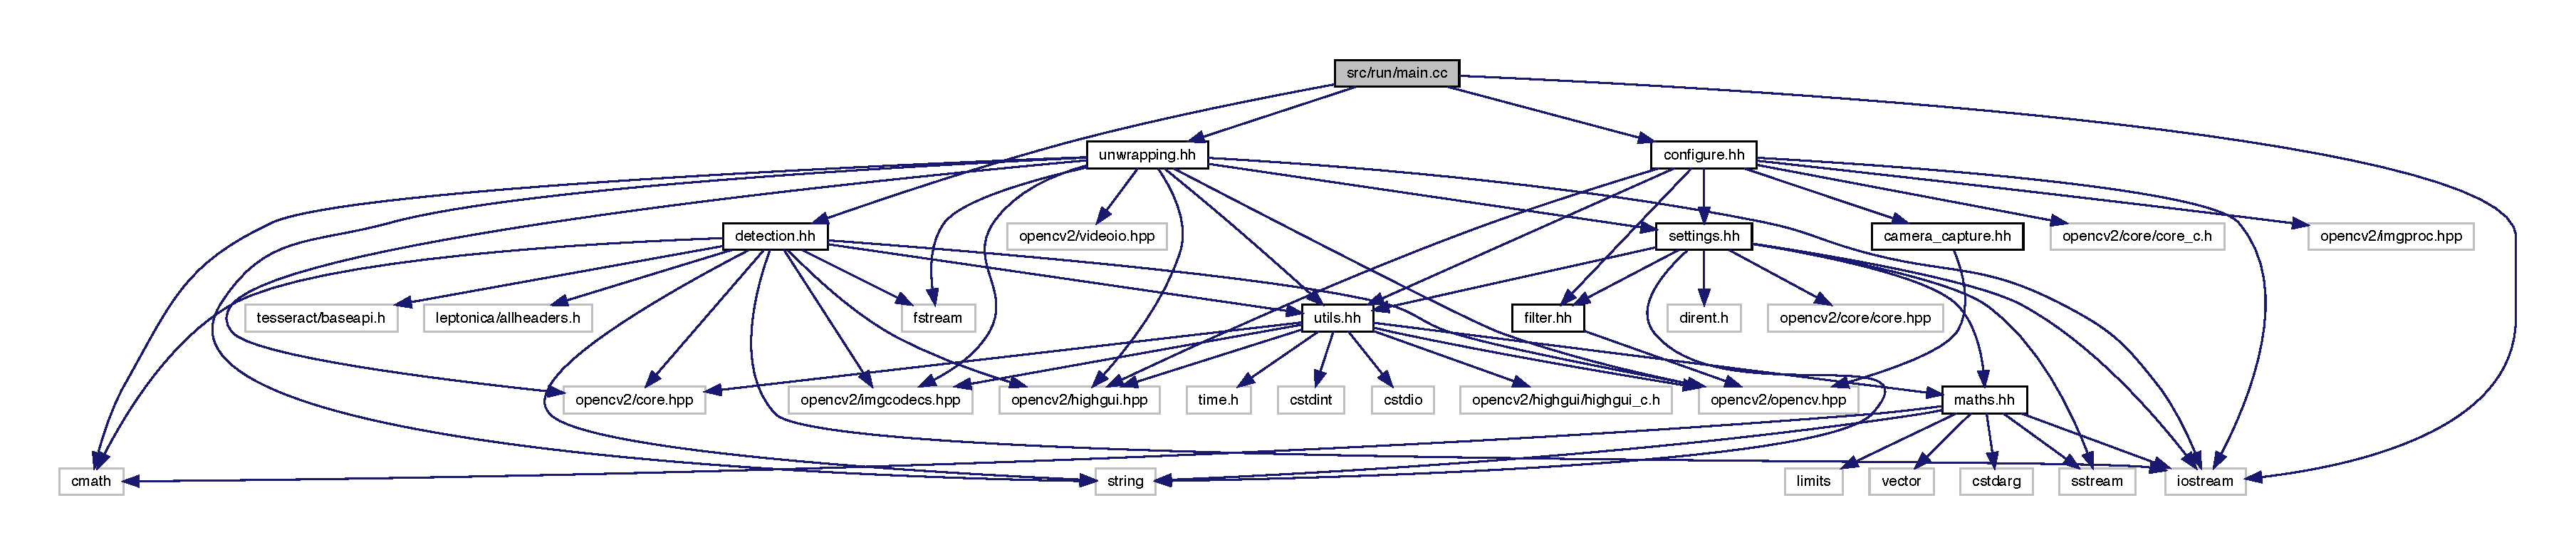
\includegraphics[width=350pt]{main_8cc__incl}
\end{center}
\end{figure}
\subsection*{Functions}
\begin{DoxyCompactItemize}
\item 
\mbox{\hyperlink{draw_8hh_aa620a13339ac3a1177c86edc549fda9b}{int}} \mbox{\hyperlink{main_8cc_ae66f6b31b5ad750f1fe042a706a4e3d4}{main}} ()
\end{DoxyCompactItemize}


\subsection{Function Documentation}
\mbox{\Hypertarget{main_8cc_ae66f6b31b5ad750f1fe042a706a4e3d4}\label{main_8cc_ae66f6b31b5ad750f1fe042a706a4e3d4}} 
\index{main.cc@{main.cc}!main@{main}}
\index{main@{main}!main.cc@{main.cc}}
\subsubsection{\texorpdfstring{main()}{main()}}
{\footnotesize\ttfamily \mbox{\hyperlink{draw_8hh_aa620a13339ac3a1177c86edc549fda9b}{int}} main (\begin{DoxyParamCaption}{ }\end{DoxyParamCaption})}


\hypertarget{unwrapping_8cc}{}\section{src/unwrapping.cc File Reference}
\label{unwrapping_8cc}\index{src/unwrapping.cc@{src/unwrapping.cc}}
{\ttfamily \#include \char`\"{}unwrapping.\+hh\char`\"{}}\newline
Include dependency graph for unwrapping.\+cc\+:
\nopagebreak
\begin{figure}[H]
\begin{center}
\leavevmode
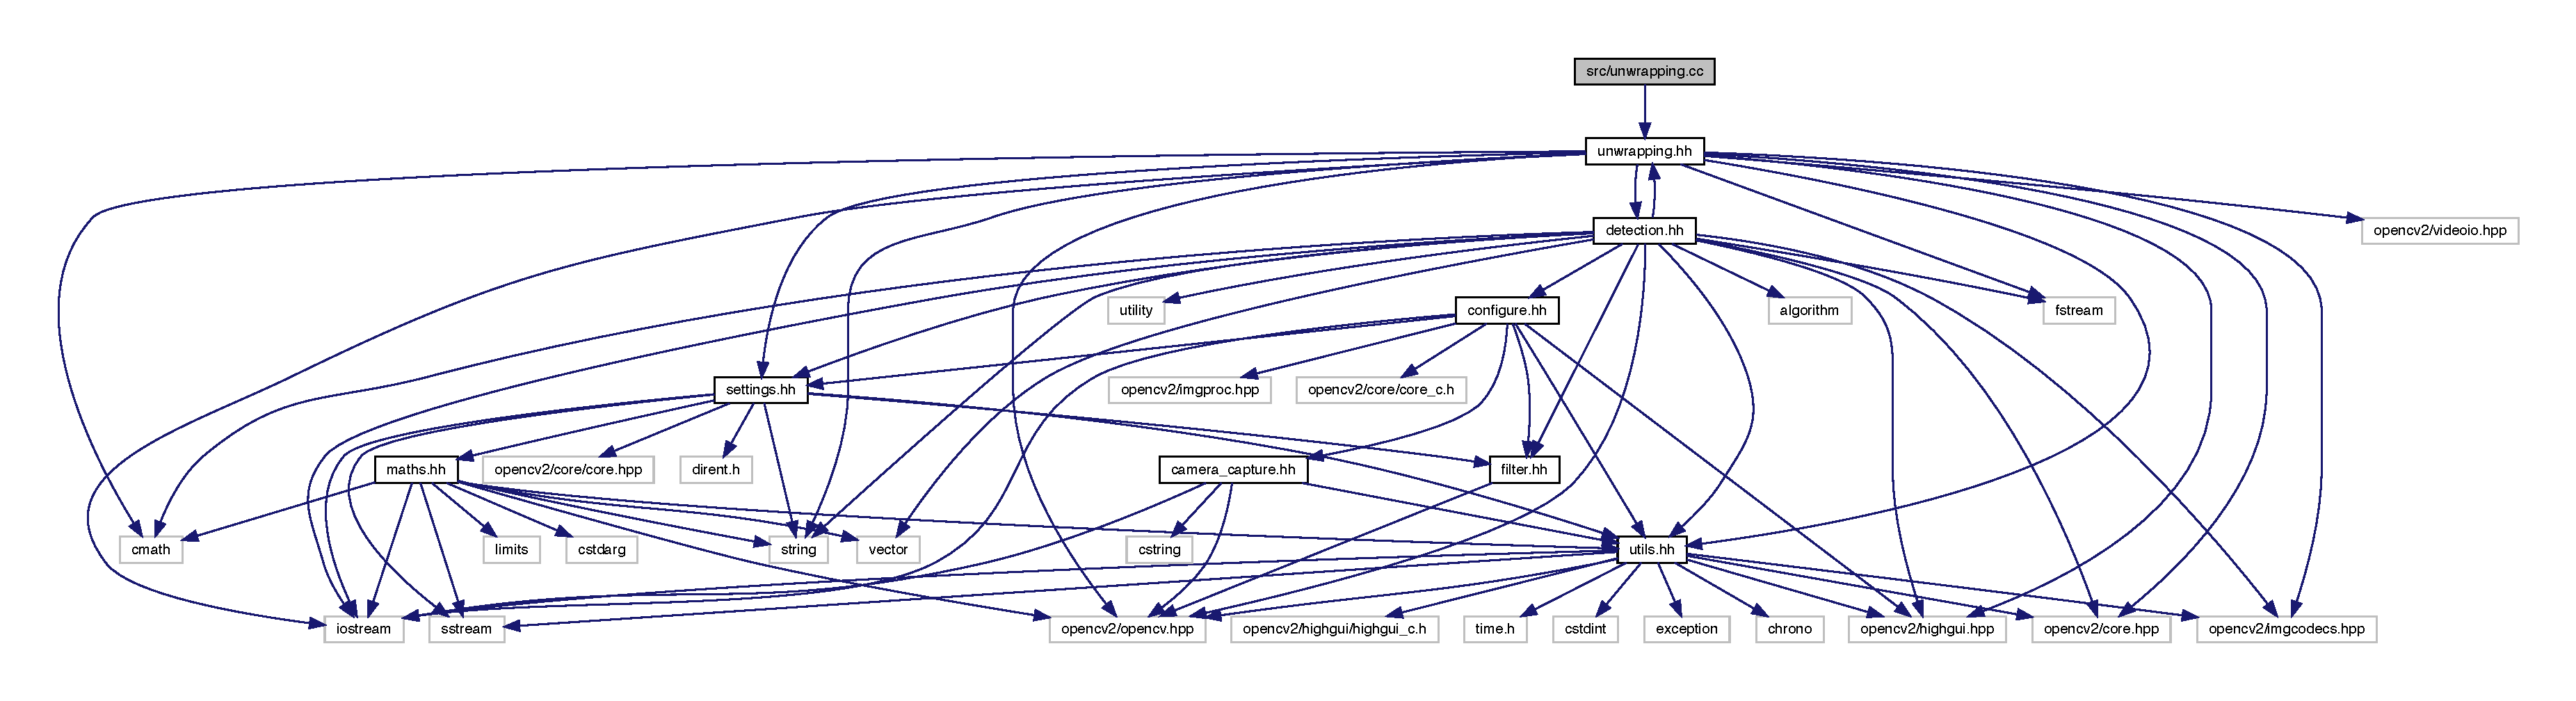
\includegraphics[width=350pt]{unwrapping_8cc__incl}
\end{center}
\end{figure}
\subsection*{Macros}
\begin{DoxyCompactItemize}
\item 
\#define \mbox{\hyperlink{unwrapping_8cc_a3c7ffff21a9a31fea3e9777b02d09291}{A\+R\+E\+A\+\_\+\+R\+A\+T\+IO}}~0.\+7
\item 
\#define \mbox{\hyperlink{unwrapping_8cc_ac2f75959ffa14bc8fd8d0491e890c122}{A\+R\+E\+A\+\_\+\+M\+IN}}~500
\end{DoxyCompactItemize}
\subsection*{Functions}
\begin{DoxyCompactItemize}
\item 
static float \mbox{\hyperlink{unwrapping_8cc_ac6bcc6db62057bda0b6195a11578fdfa}{distance}} (Point c1, Point c2)
\begin{DoxyCompactList}\small\item\em Compute the euclidean distance. \end{DoxyCompactList}\item 
\mbox{\hyperlink{draw_8hh_aa620a13339ac3a1177c86edc549fda9b}{int}} \mbox{\hyperlink{unwrapping_8cc_ae232c3264987d57a223a39226929da29}{unwrapping}} ()
\begin{DoxyCompactList}\small\item\em Take some images according to a xml and unwrap the black rectangle inside the image after appling undistortion trasformation. \end{DoxyCompactList}\item 
void \mbox{\hyperlink{unwrapping_8cc_ac30b4dbae9022e84e10ef97ba156c581}{find\+\_\+rect}} (vector$<$ Point $>$ \&\+\_\+rect, const \mbox{\hyperlink{draw_8hh_aa620a13339ac3a1177c86edc549fda9b}{int}} \&width, const \mbox{\hyperlink{draw_8hh_aa620a13339ac3a1177c86edc549fda9b}{int}} \&height)
\begin{DoxyCompactList}\small\item\em Since the border of the arena might not always be clean but might have some imperfection, this functions computes the four vertixes taking all the points and computing the four that are the clostest to the corner of the image. \end{DoxyCompactList}\item 
void \mbox{\hyperlink{unwrapping_8cc_a3cf7df08897ed4d1a7ddcf055b18cca8}{load\+Coefficients}} (const string filename, Mat \&camera\+\_\+matrix, Mat \&dist\+\_\+coeffs)
\begin{DoxyCompactList}\small\item\em Load coefficients from a file. \end{DoxyCompactList}\end{DoxyCompactItemize}


\subsection{Macro Definition Documentation}
\mbox{\Hypertarget{unwrapping_8cc_ac2f75959ffa14bc8fd8d0491e890c122}\label{unwrapping_8cc_ac2f75959ffa14bc8fd8d0491e890c122}} 
\index{unwrapping.cc@{unwrapping.cc}!AREA\_MIN@{AREA\_MIN}}
\index{AREA\_MIN@{AREA\_MIN}!unwrapping.cc@{unwrapping.cc}}
\subsubsection{\texorpdfstring{AREA\_MIN}{AREA\_MIN}}
{\footnotesize\ttfamily \#define A\+R\+E\+A\+\_\+\+M\+IN~500}

\mbox{\Hypertarget{unwrapping_8cc_a3c7ffff21a9a31fea3e9777b02d09291}\label{unwrapping_8cc_a3c7ffff21a9a31fea3e9777b02d09291}} 
\index{unwrapping.cc@{unwrapping.cc}!AREA\_RATIO@{AREA\_RATIO}}
\index{AREA\_RATIO@{AREA\_RATIO}!unwrapping.cc@{unwrapping.cc}}
\subsubsection{\texorpdfstring{AREA\_RATIO}{AREA\_RATIO}}
{\footnotesize\ttfamily \#define A\+R\+E\+A\+\_\+\+R\+A\+T\+IO~0.\+7}



\subsection{Function Documentation}
\mbox{\Hypertarget{unwrapping_8cc_ac6bcc6db62057bda0b6195a11578fdfa}\label{unwrapping_8cc_ac6bcc6db62057bda0b6195a11578fdfa}} 
\index{unwrapping.cc@{unwrapping.cc}!distance@{distance}}
\index{distance@{distance}!unwrapping.cc@{unwrapping.cc}}
\subsubsection{\texorpdfstring{distance()}{distance()}}
{\footnotesize\ttfamily static float distance (\begin{DoxyParamCaption}\item[{Point}]{c1,  }\item[{Point}]{c2 }\end{DoxyParamCaption})\hspace{0.3cm}{\ttfamily [static]}}



Compute the euclidean distance. 


\begin{DoxyParams}[1]{Parameters}
\mbox{\texttt{ in,out}}  & {\em c1} & The first point. \\
\hline
\mbox{\texttt{ in,out}}  & {\em c2} & The second point.\\
\hline
\end{DoxyParams}
\begin{DoxyReturn}{Returns}
The euclidean distance. 
\end{DoxyReturn}
\mbox{\Hypertarget{unwrapping_8cc_ac30b4dbae9022e84e10ef97ba156c581}\label{unwrapping_8cc_ac30b4dbae9022e84e10ef97ba156c581}} 
\index{unwrapping.cc@{unwrapping.cc}!find\_rect@{find\_rect}}
\index{find\_rect@{find\_rect}!unwrapping.cc@{unwrapping.cc}}
\subsubsection{\texorpdfstring{find\_rect()}{find\_rect()}}
{\footnotesize\ttfamily void find\+\_\+rect (\begin{DoxyParamCaption}\item[{vector$<$ Point $>$ \&}]{\+\_\+rect,  }\item[{const \mbox{\hyperlink{draw_8hh_aa620a13339ac3a1177c86edc549fda9b}{int}} \&}]{width,  }\item[{const \mbox{\hyperlink{draw_8hh_aa620a13339ac3a1177c86edc549fda9b}{int}} \&}]{height }\end{DoxyParamCaption})}



Since the border of the arena might not always be clean but might have some imperfection, this functions computes the four vertixes taking all the points and computing the four that are the clostest to the corner of the image. 


\begin{DoxyParams}[1]{Parameters}
\mbox{\texttt{ in}}  & {\em \+\_\+rect} & The vector of cv\+::\+Point to work on. \\
\hline
\mbox{\texttt{ in}}  & {\em width} & The width of the image. \\
\hline
\mbox{\texttt{ in}}  & {\em height} & The height of the image. \\
\hline
\end{DoxyParams}
\mbox{\Hypertarget{unwrapping_8cc_a3cf7df08897ed4d1a7ddcf055b18cca8}\label{unwrapping_8cc_a3cf7df08897ed4d1a7ddcf055b18cca8}} 
\index{unwrapping.cc@{unwrapping.cc}!loadCoefficients@{loadCoefficients}}
\index{loadCoefficients@{loadCoefficients}!unwrapping.cc@{unwrapping.cc}}
\subsubsection{\texorpdfstring{loadCoefficients()}{loadCoefficients()}}
{\footnotesize\ttfamily void load\+Coefficients (\begin{DoxyParamCaption}\item[{const string}]{filename,  }\item[{Mat \&}]{camera\+\_\+matrix,  }\item[{Mat \&}]{dist\+\_\+coeffs }\end{DoxyParamCaption})}



Load coefficients from a file. 

Load two matrix \textquotesingle{}camera\+\_\+matrix\textquotesingle{} and \textquotesingle{}distortion\+\_\+coefficients\textquotesingle{} from the xml file passed. 
\begin{DoxyParams}[1]{Parameters}
\mbox{\texttt{ in}}  & {\em filename} & The string that identify the location of the xml file. \\
\hline
\mbox{\texttt{ out}}  & {\em camera\+\_\+matrix} & Where the \textquotesingle{}camera\+\_\+matrix\textquotesingle{} matrix is saved. \\
\hline
\mbox{\texttt{ out}}  & {\em dist\+\_\+coeffs} & Where the \textquotesingle{}distortion\+\_\+coefficients\textquotesingle{} matrix is saved. \\
\hline
\end{DoxyParams}
\mbox{\Hypertarget{unwrapping_8cc_ae232c3264987d57a223a39226929da29}\label{unwrapping_8cc_ae232c3264987d57a223a39226929da29}} 
\index{unwrapping.cc@{unwrapping.cc}!unwrapping@{unwrapping}}
\index{unwrapping@{unwrapping}!unwrapping.cc@{unwrapping.cc}}
\subsubsection{\texorpdfstring{unwrapping()}{unwrapping()}}
{\footnotesize\ttfamily \mbox{\hyperlink{draw_8hh_aa620a13339ac3a1177c86edc549fda9b}{int}} unwrapping (\begin{DoxyParamCaption}{ }\end{DoxyParamCaption})}



Take some images according to a xml and unwrap the black rectangle inside the image after appling undistortion trasformation. 

Load from the xml file \textquotesingle{}data/settings.\+xml\textquotesingle{} the name of some images, load the images from the file,~\newline
apply the calibration (undistortion trasformation) thanks to the matrices load with the \textquotesingle{}load\+Coefficients\textquotesingle{} function.~\newline
Then, with the use of a filter for the black the region of interest (a rectangle) is identified and all the perspective is rotated for reach a top view of the rectangle.~\newline
Finally, the images are saved on some files.

\begin{DoxyReturn}{Returns}
A 0 is return if the function reach the end. 
\end{DoxyReturn}

\hypertarget{unwrapping_8hh}{}\section{src/include/unwrapping.hh File Reference}
\label{unwrapping_8hh}\index{src/include/unwrapping.hh@{src/include/unwrapping.hh}}
{\ttfamily \#include $<$utils.\+hh$>$}\newline
{\ttfamily \#include $<$settings.\+hh$>$}\newline
{\ttfamily \#include $<$iostream$>$}\newline
{\ttfamily \#include $<$fstream$>$}\newline
{\ttfamily \#include $<$string$>$}\newline
{\ttfamily \#include $<$cmath$>$}\newline
{\ttfamily \#include $<$opencv2/videoio.\+hpp$>$}\newline
{\ttfamily \#include $<$opencv2/highgui.\+hpp$>$}\newline
{\ttfamily \#include $<$opencv2/core.\+hpp$>$}\newline
{\ttfamily \#include $<$opencv2/opencv.\+hpp$>$}\newline
{\ttfamily \#include $<$opencv2/imgcodecs.\+hpp$>$}\newline
Include dependency graph for unwrapping.\+hh\+:
\nopagebreak
\begin{figure}[H]
\begin{center}
\leavevmode
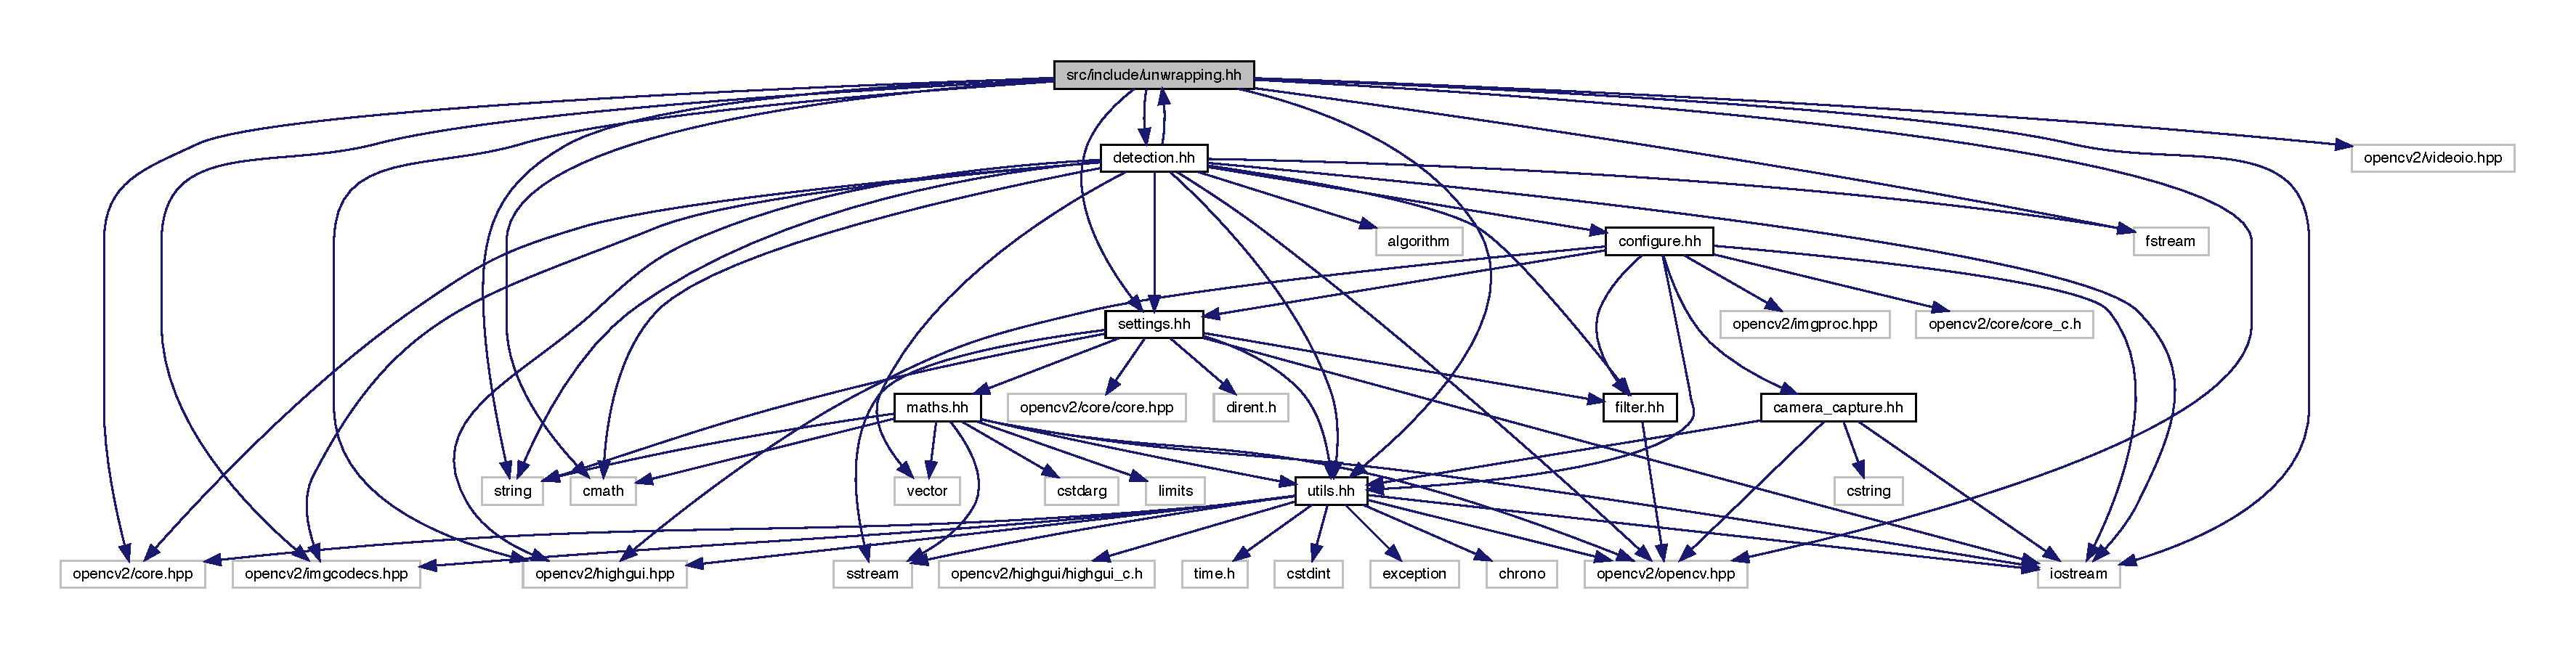
\includegraphics[width=350pt]{unwrapping_8hh__incl}
\end{center}
\end{figure}
This graph shows which files directly or indirectly include this file\+:
\nopagebreak
\begin{figure}[H]
\begin{center}
\leavevmode
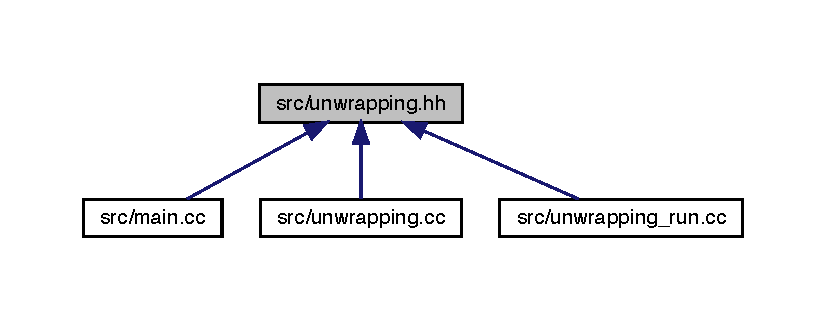
\includegraphics[width=350pt]{unwrapping_8hh__dep__incl}
\end{center}
\end{figure}
\subsection*{Functions}
\begin{DoxyCompactItemize}
\item 
\mbox{\hyperlink{draw_8hh_aa620a13339ac3a1177c86edc549fda9b}{int}} \mbox{\hyperlink{unwrapping_8hh_ae232c3264987d57a223a39226929da29}{unwrapping}} ()
\begin{DoxyCompactList}\small\item\em Take some images according to a xml and unwrap the black rectangle inside the image after appling undistortion trasformation. \end{DoxyCompactList}\item 
void \mbox{\hyperlink{unwrapping_8hh_a3cf7df08897ed4d1a7ddcf055b18cca8}{load\+Coefficients}} (const string filename, Mat \&camera\+\_\+matrix, Mat \&dist\+\_\+coeffs)
\begin{DoxyCompactList}\small\item\em Load coefficients from a file. \end{DoxyCompactList}\end{DoxyCompactItemize}


\subsection{Function Documentation}
\mbox{\Hypertarget{unwrapping_8hh_a3cf7df08897ed4d1a7ddcf055b18cca8}\label{unwrapping_8hh_a3cf7df08897ed4d1a7ddcf055b18cca8}} 
\index{unwrapping.hh@{unwrapping.hh}!loadCoefficients@{loadCoefficients}}
\index{loadCoefficients@{loadCoefficients}!unwrapping.hh@{unwrapping.hh}}
\subsubsection{\texorpdfstring{loadCoefficients()}{loadCoefficients()}}
{\footnotesize\ttfamily void load\+Coefficients (\begin{DoxyParamCaption}\item[{const string}]{filename,  }\item[{Mat \&}]{camera\+\_\+matrix,  }\item[{Mat \&}]{dist\+\_\+coeffs }\end{DoxyParamCaption})}



Load coefficients from a file. 

Load two matrix \textquotesingle{}camera\+\_\+matrix\textquotesingle{} and \textquotesingle{}distortion\+\_\+coefficients\textquotesingle{} from the xml file passed. 
\begin{DoxyParams}[1]{Parameters}
\mbox{\texttt{ in}}  & {\em filename} & The string that identify the location of the xml file. \\
\hline
\mbox{\texttt{ out}}  & {\em camera\+\_\+matrix} & Where the \textquotesingle{}camera\+\_\+matrix\textquotesingle{} matrix is saved. \\
\hline
\mbox{\texttt{ out}}  & {\em dist\+\_\+coeffs} & Where the \textquotesingle{}distortion\+\_\+coefficients\textquotesingle{} matrix is saved. \\
\hline
\end{DoxyParams}
\mbox{\Hypertarget{unwrapping_8hh_ae232c3264987d57a223a39226929da29}\label{unwrapping_8hh_ae232c3264987d57a223a39226929da29}} 
\index{unwrapping.hh@{unwrapping.hh}!unwrapping@{unwrapping}}
\index{unwrapping@{unwrapping}!unwrapping.hh@{unwrapping.hh}}
\subsubsection{\texorpdfstring{unwrapping()}{unwrapping()}}
{\footnotesize\ttfamily \mbox{\hyperlink{draw_8hh_aa620a13339ac3a1177c86edc549fda9b}{int}} unwrapping (\begin{DoxyParamCaption}{ }\end{DoxyParamCaption})}



Take some images according to a xml and unwrap the black rectangle inside the image after appling undistortion trasformation. 

Load from the xml file \textquotesingle{}data/settings.\+xml\textquotesingle{} the name of some images, load the images from the file,~\newline
apply the calibration (undistortion trasformation) thanks to the matrices load with the \textquotesingle{}load\+Coefficients\textquotesingle{} function.~\newline
Then, with the use of a filter for the black the region of interest (a rectangle) is identified and all the perspective is rotated for reach a top view of the rectangle.~\newline
Finally, the images are saved on some files.

\begin{DoxyReturn}{Returns}
A 0 is return if the function reach the end. 
\end{DoxyReturn}
File\+Storage fs\+\_\+xml(xml\+\_\+settings, File\+Storage\+::\+R\+E\+A\+D);

File\+Node Bm = s-\/$>$black\+Mask; 
\hypertarget{unwrapping__run_8cc}{}\section{src/run/unwrapping\+\_\+run.cc File Reference}
\label{unwrapping__run_8cc}\index{src/run/unwrapping\_run.cc@{src/run/unwrapping\_run.cc}}
{\ttfamily \#include $<$unwrapping.\+hh$>$}\newline
Include dependency graph for unwrapping\+\_\+run.\+cc\+:
\nopagebreak
\begin{figure}[H]
\begin{center}
\leavevmode
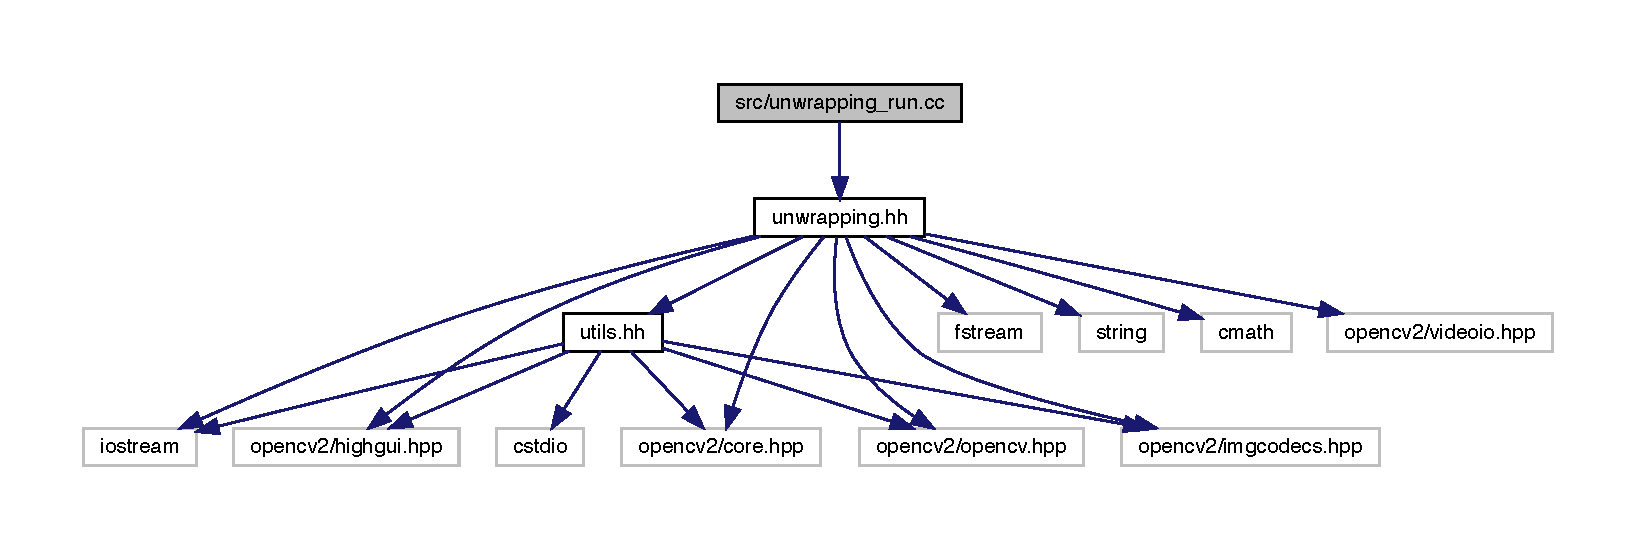
\includegraphics[width=350pt]{unwrapping__run_8cc__incl}
\end{center}
\end{figure}
\subsection*{Functions}
\begin{DoxyCompactItemize}
\item 
\mbox{\hyperlink{draw_8hh_aa620a13339ac3a1177c86edc549fda9b}{int}} \mbox{\hyperlink{unwrapping__run_8cc_ae66f6b31b5ad750f1fe042a706a4e3d4}{main}} ()
\end{DoxyCompactItemize}


\subsection{Function Documentation}
\mbox{\Hypertarget{unwrapping__run_8cc_ae66f6b31b5ad750f1fe042a706a4e3d4}\label{unwrapping__run_8cc_ae66f6b31b5ad750f1fe042a706a4e3d4}} 
\index{unwrapping\_run.cc@{unwrapping\_run.cc}!main@{main}}
\index{main@{main}!unwrapping\_run.cc@{unwrapping\_run.cc}}
\subsubsection{\texorpdfstring{main()}{main()}}
{\footnotesize\ttfamily \mbox{\hyperlink{draw_8hh_aa620a13339ac3a1177c86edc549fda9b}{int}} main (\begin{DoxyParamCaption}{ }\end{DoxyParamCaption})}


\hypertarget{utils_8cc}{}\section{src/utils.cc File Reference}
\label{utils_8cc}\index{src/utils.\+cc@{src/utils.\+cc}}
{\ttfamily \#include \char`\"{}utils.\+hh\char`\"{}}\newline
Include dependency graph for utils.\+cc\+:
\nopagebreak
\begin{figure}[H]
\begin{center}
\leavevmode
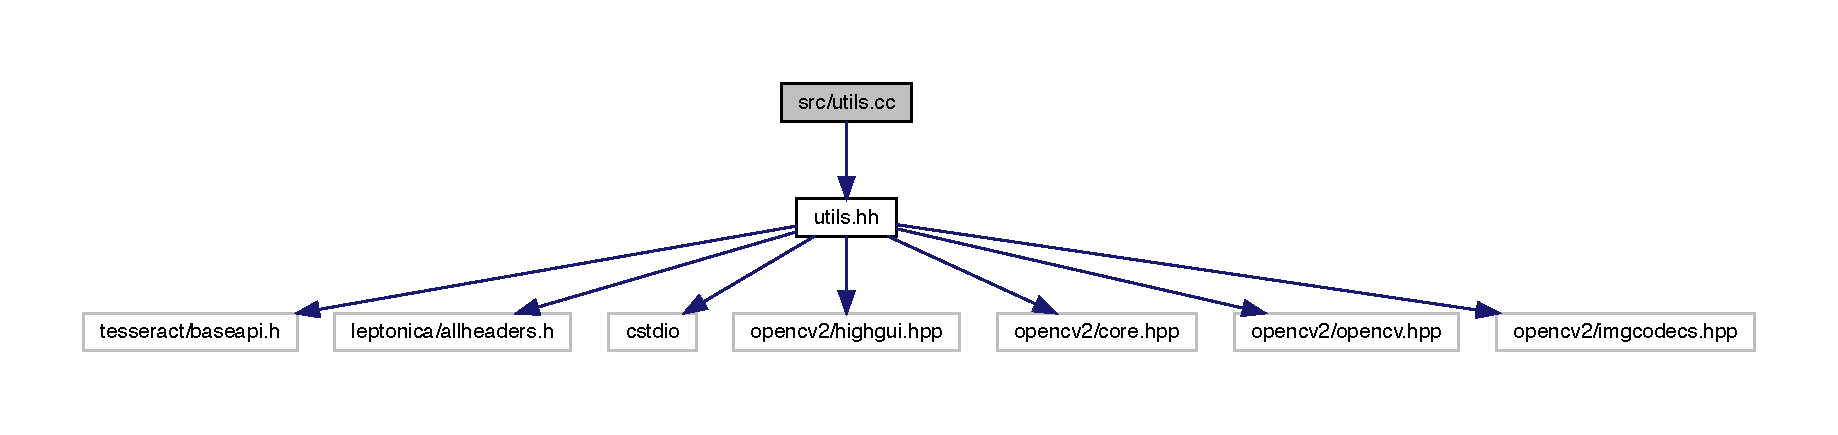
\includegraphics[width=350pt]{utils_8cc__incl}
\end{center}
\end{figure}
\subsection*{Functions}
\begin{DoxyCompactItemize}
\item 
void \mbox{\hyperlink{utils_8cc_a9a82362cf25a772ae278a98a68464c1f}{my\+\_\+imshow}} (const char $\ast$win\+\_\+name, Mat img, bool reset)
\end{DoxyCompactItemize}


\subsection{Function Documentation}
\mbox{\Hypertarget{utils_8cc_a9a82362cf25a772ae278a98a68464c1f}\label{utils_8cc_a9a82362cf25a772ae278a98a68464c1f}} 
\index{utils.\+cc@{utils.\+cc}!my\+\_\+imshow@{my\+\_\+imshow}}
\index{my\+\_\+imshow@{my\+\_\+imshow}!utils.\+cc@{utils.\+cc}}
\subsubsection{\texorpdfstring{my\+\_\+imshow()}{my\_imshow()}}
{\footnotesize\ttfamily void my\+\_\+imshow (\begin{DoxyParamCaption}\item[{const char $\ast$}]{win\+\_\+name,  }\item[{Mat}]{img,  }\item[{bool}]{reset }\end{DoxyParamCaption})}


\hypertarget{utils_8hh}{}\section{src/include/utils.hh File Reference}
\label{utils_8hh}\index{src/include/utils.hh@{src/include/utils.hh}}
{\ttfamily \#include $<$sstream$>$}\newline
{\ttfamily \#include $<$iostream$>$}\newline
{\ttfamily \#include $<$exception$>$}\newline
{\ttfamily \#include $<$chrono$>$}\newline
{\ttfamily \#include $<$opencv2/highgui.\+hpp$>$}\newline
{\ttfamily \#include $<$opencv2/highgui/highgui\+\_\+c.\+h$>$}\newline
{\ttfamily \#include $<$opencv2/core.\+hpp$>$}\newline
{\ttfamily \#include $<$opencv2/opencv.\+hpp$>$}\newline
{\ttfamily \#include $<$opencv2/imgcodecs.\+hpp$>$}\newline
{\ttfamily \#include $<$time.\+h$>$}\newline
{\ttfamily \#include $<$cstdint$>$}\newline
Include dependency graph for utils.\+hh\+:
\nopagebreak
\begin{figure}[H]
\begin{center}
\leavevmode
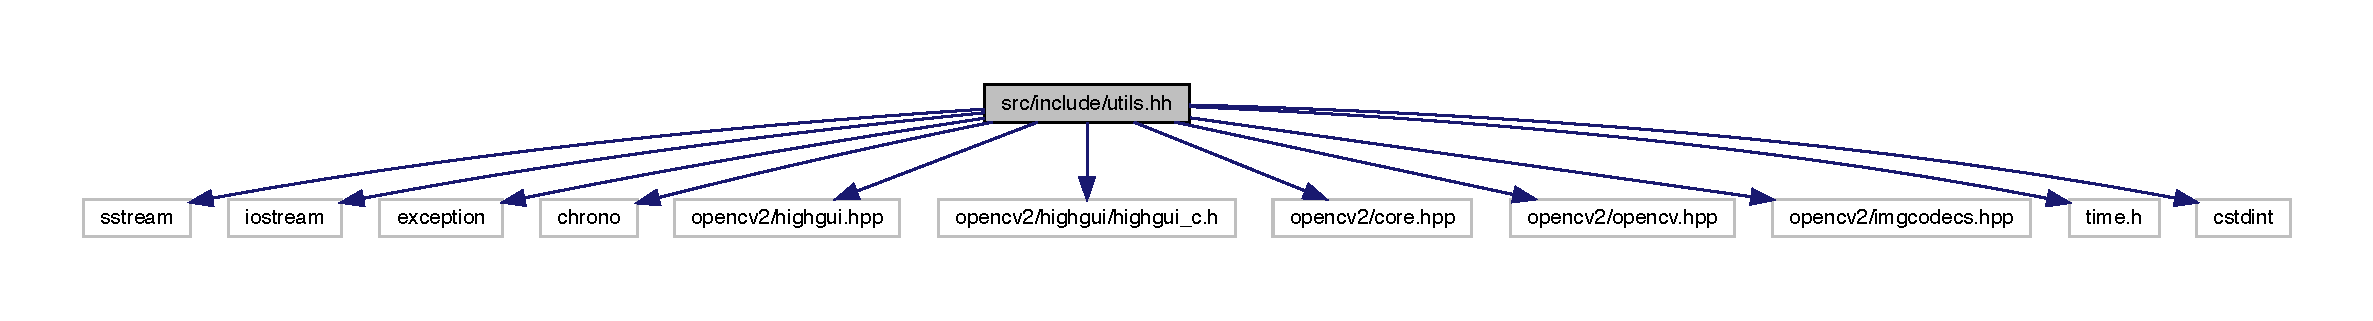
\includegraphics[width=350pt]{utils_8hh__incl}
\end{center}
\end{figure}
This graph shows which files directly or indirectly include this file\+:
\nopagebreak
\begin{figure}[H]
\begin{center}
\leavevmode
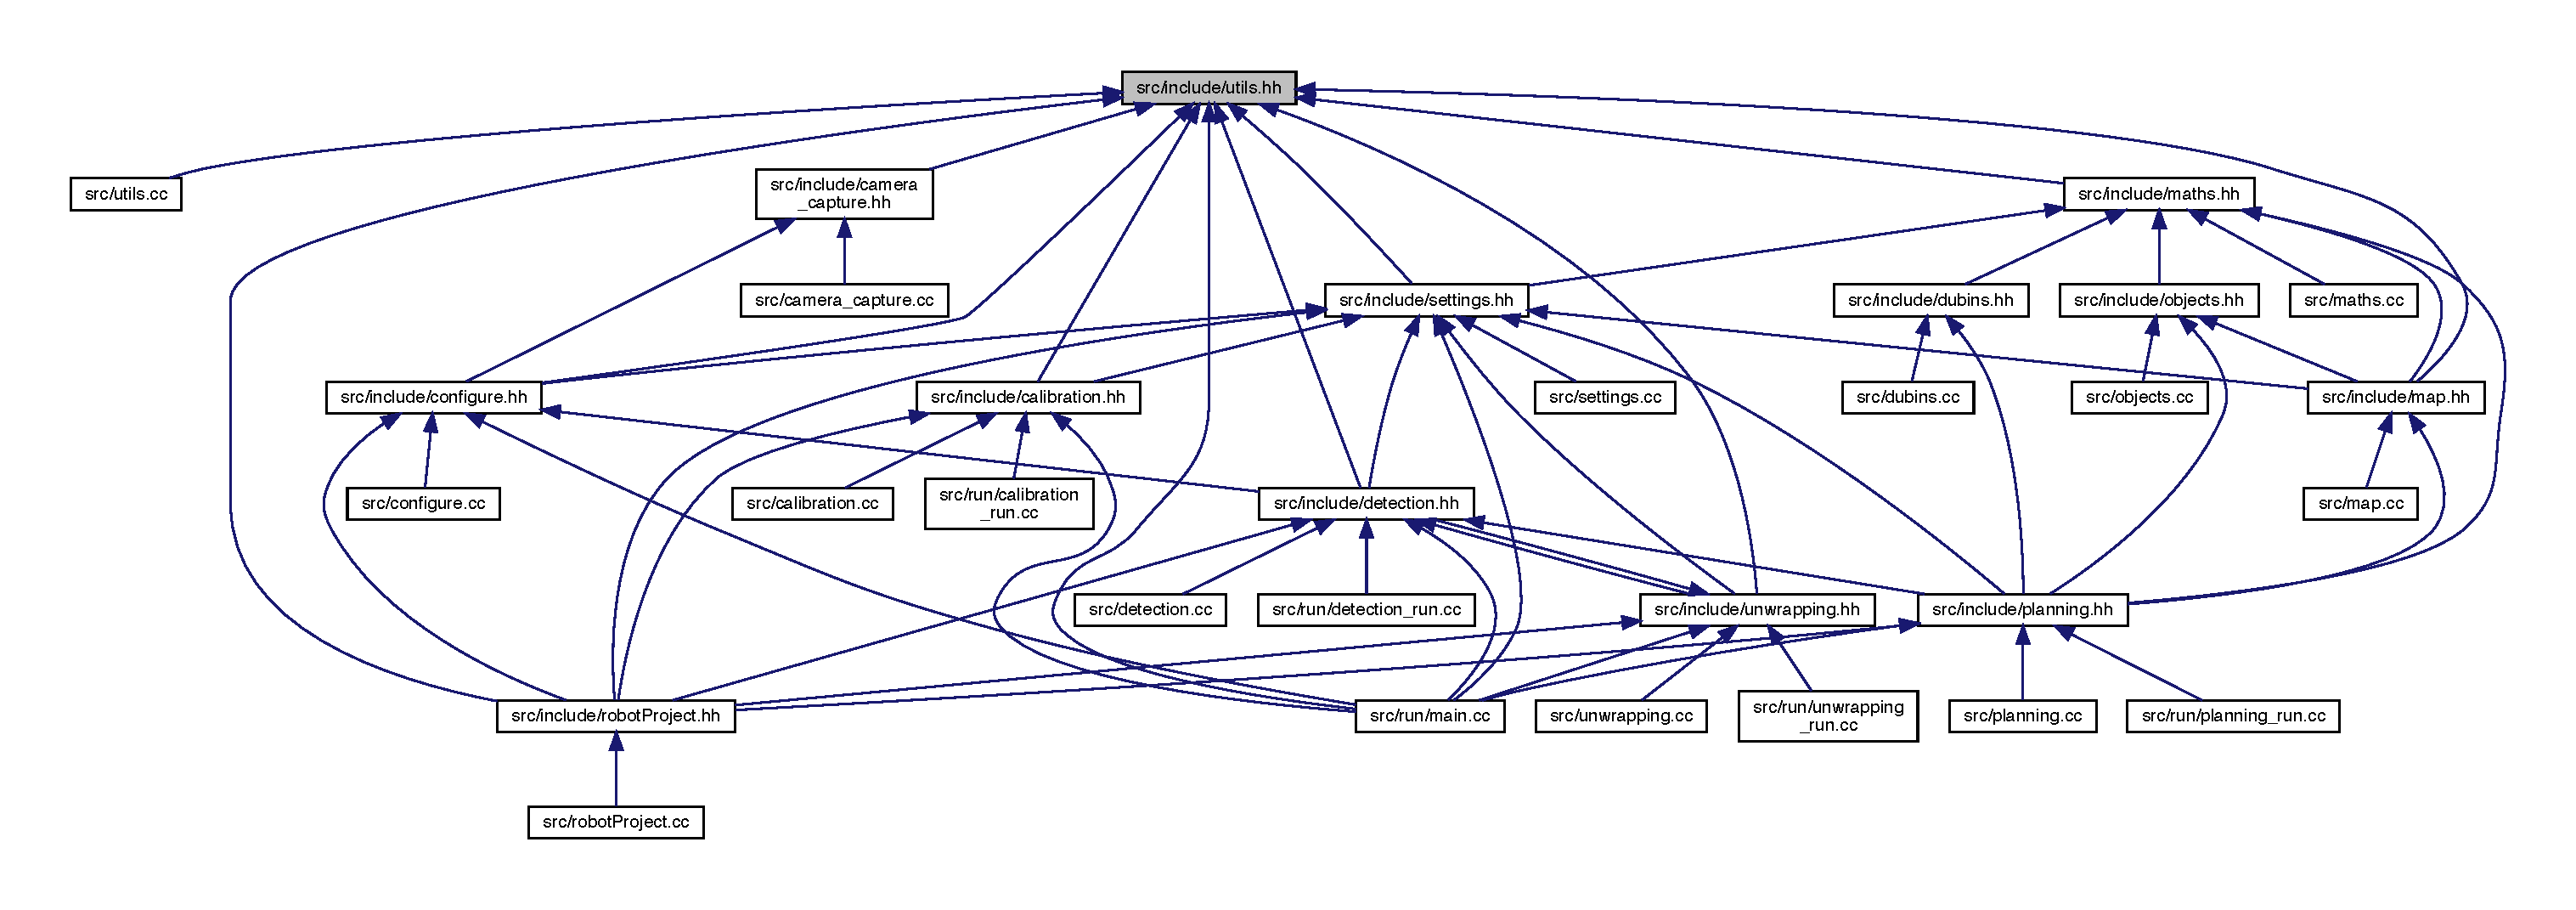
\includegraphics[width=350pt]{utils_8hh__dep__incl}
\end{center}
\end{figure}
\subsection*{Classes}
\begin{DoxyCompactItemize}
\item 
class \mbox{\hyperlink{class_my_exception}{My\+Exception$<$ T $>$}}
\end{DoxyCompactItemize}
\subsection*{Namespaces}
\begin{DoxyCompactItemize}
\item 
 \mbox{\hyperlink{namespace_c_h_r_o_n_o}{C\+H\+R\+O\+NO}}
\item 
 \mbox{\hyperlink{namespacetimeutils}{timeutils}}
\end{DoxyCompactItemize}
\subsection*{Macros}
\begin{DoxyCompactItemize}
\item 
\#define \mbox{\hyperlink{utils_8hh_a14111ac8f43949172b152e50dc720aba}{N\+A\+ME}}(x)~\#x
\begin{DoxyCompactList}\small\item\em Returns the name of the variable. \end{DoxyCompactList}\item 
\#define \mbox{\hyperlink{utils_8hh_a051dcff3fa35db18fbabb4fde1bd1167}{C\+O\+UT}}(x)
\begin{DoxyCompactList}\small\item\em Print a messag to stderr. \end{DoxyCompactList}\item 
\#define \mbox{\hyperlink{utils_8hh_a3ae64706314066fdc8b6c8029a915aa7}{I\+N\+FO}}(msg)
\begin{DoxyCompactList}\small\item\em Print the name of a variable and its content. Only if D\+E\+B\+UG is defined. \end{DoxyCompactList}\end{DoxyCompactItemize}
\subsection*{Typedefs}
\begin{DoxyCompactItemize}
\item 
typedef chrono\+::high\+\_\+resolution\+\_\+clock \mbox{\hyperlink{utils_8hh_af5fd44b7ee78ceeb4a0e869179f422f7}{Clock}}
\end{DoxyCompactItemize}
\subsection*{Enumerations}
\begin{DoxyCompactItemize}
\item 
enum \mbox{\hyperlink{namespace_c_h_r_o_n_o_a246e471488a6e6b17ddb86e3b817c7d9}{C\+H\+R\+O\+N\+O\+::\+T\+I\+M\+E\+\_\+\+T\+Y\+PE}} \{ \mbox{\hyperlink{namespace_c_h_r_o_n_o_a246e471488a6e6b17ddb86e3b817c7d9ac09415dca4fa7975506ab664d88b403a}{C\+H\+R\+O\+N\+O\+::\+S\+EC}}, 
\mbox{\hyperlink{namespace_c_h_r_o_n_o_a246e471488a6e6b17ddb86e3b817c7d9a2060724ab75592144c0b930e3394d845}{C\+H\+R\+O\+N\+O\+::\+M\+S\+EC}}, 
\mbox{\hyperlink{namespace_c_h_r_o_n_o_a246e471488a6e6b17ddb86e3b817c7d9aba8c3a9d281e3b934b74d5ff97a3a093}{C\+H\+R\+O\+N\+O\+::\+M\+U\+S\+EC}}, 
\mbox{\hyperlink{namespace_c_h_r_o_n_o_a246e471488a6e6b17ddb86e3b817c7d9a06ab3311d8f423104c3beae640896013}{C\+H\+R\+O\+N\+O\+::\+N\+S\+EC}}
 \}
\item 
enum \mbox{\hyperlink{utils_8hh_af26a5d951fd6ab4b44e6cd8425aa0383}{E\+X\+C\+E\+P\+T\+I\+O\+N\+\_\+\+T\+Y\+PE}} \{ \mbox{\hyperlink{utils_8hh_af26a5d951fd6ab4b44e6cd8425aa0383aa965658e6a84d5502df1c1987b0a8466}{G\+E\+N\+E\+R\+AL}}, 
\mbox{\hyperlink{utils_8hh_af26a5d951fd6ab4b44e6cd8425aa0383a3197625a1bb2264943f5a95f236d9973}{E\+X\+I\+S\+TS}}, 
\mbox{\hyperlink{utils_8hh_af26a5d951fd6ab4b44e6cd8425aa0383a4aa71180778b711338785695df5d7c52}{S\+I\+ZE}}
 \}
\end{DoxyCompactItemize}
\subsection*{Functions}
\begin{DoxyCompactItemize}
\item 
string \mbox{\hyperlink{namespace_c_h_r_o_n_o_ae2a3e41f8bf5f83ba84d3f4d2eed3836}{C\+H\+R\+O\+N\+O\+::get\+Type}} (T\+I\+M\+E\+\_\+\+T\+Y\+PE type, string ret=\char`\"{}\char`\"{})
\item 
double \mbox{\hyperlink{namespace_c_h_r_o_n_o_aebe2329c142a6f06b6fede41c3abf1b3}{C\+H\+R\+O\+N\+O\+::get\+Elapsed}} (Clock\+::time\+\_\+point start, Clock\+::time\+\_\+point stop, T\+I\+M\+E\+\_\+\+T\+Y\+PE type=M\+U\+S\+EC)
\item 
string \mbox{\hyperlink{namespace_c_h_r_o_n_o_ad8da7180c420d59f4c0077b60579c0ae}{C\+H\+R\+O\+N\+O\+::get\+Elapsed}} (Clock\+::time\+\_\+point start, Clock\+::time\+\_\+point stop, string ret, T\+I\+M\+E\+\_\+\+T\+Y\+PE type=M\+U\+S\+EC)
\item 
void \mbox{\hyperlink{utils_8hh_aabfea83501dfccfa4c420b8c19ceefd7}{my\+\_\+imshow}} (const char $\ast$win\+\_\+name, Mat img, bool reset=false)
\begin{DoxyCompactList}\small\item\em Function to show images in an order grill. \end{DoxyCompactList}\item 
void \mbox{\hyperlink{utils_8hh_af046ae860c3e4985ab0968caffb4c772}{mywaitkey}} (const char c=\textquotesingle{}q\textquotesingle{})
\begin{DoxyCompactList}\small\item\em Function to use after \mbox{\hyperlink{utils_8hh_aabfea83501dfccfa4c420b8c19ceefd7}{my\+\_\+imshow()}} for keeping the image opened until a key is pressed. \end{DoxyCompactList}\item 
void \mbox{\hyperlink{utils_8hh_a31ae190fba03c3a422a13a4271e0e424}{mywaitkey}} (string window\+Name)
\begin{DoxyCompactList}\small\item\em Function to use after \mbox{\hyperlink{utils_8hh_aabfea83501dfccfa4c420b8c19ceefd7}{my\+\_\+imshow()}} for keeping the image opened until a key is pressed. When a key is pressed a specific window is closed. \end{DoxyCompactList}\item 
int64\+\_\+t \mbox{\hyperlink{namespacetimeutils_a3d9d509a7028cffae8aef9c70f6c2c52}{timeutils\+::timespec\+Diff}} (struct timespec $\ast$time\+A\+\_\+p, struct timespec $\ast$time\+B\+\_\+p)
\item 
double \mbox{\hyperlink{namespacetimeutils_aa732b7f41462ff727daef77bd5030b9c}{timeutils\+::get\+TimeS}} ()
\end{DoxyCompactItemize}


\subsection{Macro Definition Documentation}
\mbox{\Hypertarget{utils_8hh_a051dcff3fa35db18fbabb4fde1bd1167}\label{utils_8hh_a051dcff3fa35db18fbabb4fde1bd1167}} 
\index{utils.hh@{utils.hh}!COUT@{COUT}}
\index{COUT@{COUT}!utils.hh@{utils.hh}}
\subsubsection{\texorpdfstring{COUT}{COUT}}
{\footnotesize\ttfamily \#define C\+O\+UT(\begin{DoxyParamCaption}\item[{}]{x }\end{DoxyParamCaption})}



Print a messag to stderr. 

\mbox{\Hypertarget{utils_8hh_a3ae64706314066fdc8b6c8029a915aa7}\label{utils_8hh_a3ae64706314066fdc8b6c8029a915aa7}} 
\index{utils.hh@{utils.hh}!INFO@{INFO}}
\index{INFO@{INFO}!utils.hh@{utils.hh}}
\subsubsection{\texorpdfstring{INFO}{INFO}}
{\footnotesize\ttfamily \#define I\+N\+FO(\begin{DoxyParamCaption}\item[{}]{msg }\end{DoxyParamCaption})}



Print the name of a variable and its content. Only if D\+E\+B\+UG is defined. 

\mbox{\Hypertarget{utils_8hh_a14111ac8f43949172b152e50dc720aba}\label{utils_8hh_a14111ac8f43949172b152e50dc720aba}} 
\index{utils.hh@{utils.hh}!NAME@{NAME}}
\index{NAME@{NAME}!utils.hh@{utils.hh}}
\subsubsection{\texorpdfstring{NAME}{NAME}}
{\footnotesize\ttfamily \#define N\+A\+ME(\begin{DoxyParamCaption}\item[{}]{x }\end{DoxyParamCaption})~\#x}



Returns the name of the variable. 



\subsection{Typedef Documentation}
\mbox{\Hypertarget{utils_8hh_af5fd44b7ee78ceeb4a0e869179f422f7}\label{utils_8hh_af5fd44b7ee78ceeb4a0e869179f422f7}} 
\index{utils.hh@{utils.hh}!Clock@{Clock}}
\index{Clock@{Clock}!utils.hh@{utils.hh}}
\subsubsection{\texorpdfstring{Clock}{Clock}}
{\footnotesize\ttfamily typedef chrono\+::high\+\_\+resolution\+\_\+clock \mbox{\hyperlink{utils_8hh_af5fd44b7ee78ceeb4a0e869179f422f7}{Clock}}}



\subsection{Enumeration Type Documentation}
\mbox{\Hypertarget{utils_8hh_af26a5d951fd6ab4b44e6cd8425aa0383}\label{utils_8hh_af26a5d951fd6ab4b44e6cd8425aa0383}} 
\index{utils.hh@{utils.hh}!EXCEPTION\_TYPE@{EXCEPTION\_TYPE}}
\index{EXCEPTION\_TYPE@{EXCEPTION\_TYPE}!utils.hh@{utils.hh}}
\subsubsection{\texorpdfstring{EXCEPTION\_TYPE}{EXCEPTION\_TYPE}}
{\footnotesize\ttfamily enum \mbox{\hyperlink{utils_8hh_af26a5d951fd6ab4b44e6cd8425aa0383}{E\+X\+C\+E\+P\+T\+I\+O\+N\+\_\+\+T\+Y\+PE}}}

\begin{DoxyEnumFields}{Enumerator}
\raisebox{\heightof{T}}[0pt][0pt]{\index{GENERAL@{GENERAL}!utils.hh@{utils.hh}}\index{utils.hh@{utils.hh}!GENERAL@{GENERAL}}}\mbox{\Hypertarget{utils_8hh_af26a5d951fd6ab4b44e6cd8425aa0383aa965658e6a84d5502df1c1987b0a8466}\label{utils_8hh_af26a5d951fd6ab4b44e6cd8425aa0383aa965658e6a84d5502df1c1987b0a8466}} 
G\+E\+N\+E\+R\+AL&\\
\hline

\raisebox{\heightof{T}}[0pt][0pt]{\index{EXISTS@{EXISTS}!utils.hh@{utils.hh}}\index{utils.hh@{utils.hh}!EXISTS@{EXISTS}}}\mbox{\Hypertarget{utils_8hh_af26a5d951fd6ab4b44e6cd8425aa0383a3197625a1bb2264943f5a95f236d9973}\label{utils_8hh_af26a5d951fd6ab4b44e6cd8425aa0383a3197625a1bb2264943f5a95f236d9973}} 
E\+X\+I\+S\+TS&\\
\hline

\raisebox{\heightof{T}}[0pt][0pt]{\index{SIZE@{SIZE}!utils.hh@{utils.hh}}\index{utils.hh@{utils.hh}!SIZE@{SIZE}}}\mbox{\Hypertarget{utils_8hh_af26a5d951fd6ab4b44e6cd8425aa0383a4aa71180778b711338785695df5d7c52}\label{utils_8hh_af26a5d951fd6ab4b44e6cd8425aa0383a4aa71180778b711338785695df5d7c52}} 
S\+I\+ZE&\\
\hline

\end{DoxyEnumFields}


\subsection{Function Documentation}
\mbox{\Hypertarget{utils_8hh_aabfea83501dfccfa4c420b8c19ceefd7}\label{utils_8hh_aabfea83501dfccfa4c420b8c19ceefd7}} 
\index{utils.hh@{utils.hh}!my\_imshow@{my\_imshow}}
\index{my\_imshow@{my\_imshow}!utils.hh@{utils.hh}}
\subsubsection{\texorpdfstring{my\_imshow()}{my\_imshow()}}
{\footnotesize\ttfamily void my\+\_\+imshow (\begin{DoxyParamCaption}\item[{const char $\ast$}]{win\+\_\+name,  }\item[{Mat}]{img,  }\item[{bool}]{reset = {\ttfamily false} }\end{DoxyParamCaption})}



Function to show images in an order grill. 


\begin{DoxyParams}{Parameters}
{\em win\+\_\+name} & The name of the window to use. \\
\hline
{\em img} & The Mat containing the image. \\
\hline
{\em reset} & If true the image is going to be placed in 0,0 i.\+e. the top left corner of the screen. \\
\hline
\end{DoxyParams}
\mbox{\Hypertarget{utils_8hh_af046ae860c3e4985ab0968caffb4c772}\label{utils_8hh_af046ae860c3e4985ab0968caffb4c772}} 
\index{utils.hh@{utils.hh}!mywaitkey@{mywaitkey}}
\index{mywaitkey@{mywaitkey}!utils.hh@{utils.hh}}
\subsubsection{\texorpdfstring{mywaitkey()}{mywaitkey()}\hspace{0.1cm}{\footnotesize\ttfamily [1/2]}}
{\footnotesize\ttfamily void mywaitkey (\begin{DoxyParamCaption}\item[{const char}]{c }\end{DoxyParamCaption})}



Function to use after \mbox{\hyperlink{utils_8hh_aabfea83501dfccfa4c420b8c19ceefd7}{my\+\_\+imshow()}} for keeping the image opened until a key is pressed. 

\mbox{\Hypertarget{utils_8hh_a31ae190fba03c3a422a13a4271e0e424}\label{utils_8hh_a31ae190fba03c3a422a13a4271e0e424}} 
\index{utils.hh@{utils.hh}!mywaitkey@{mywaitkey}}
\index{mywaitkey@{mywaitkey}!utils.hh@{utils.hh}}
\subsubsection{\texorpdfstring{mywaitkey()}{mywaitkey()}\hspace{0.1cm}{\footnotesize\ttfamily [2/2]}}
{\footnotesize\ttfamily void mywaitkey (\begin{DoxyParamCaption}\item[{string}]{window\+Name }\end{DoxyParamCaption})}



Function to use after \mbox{\hyperlink{utils_8hh_aabfea83501dfccfa4c420b8c19ceefd7}{my\+\_\+imshow()}} for keeping the image opened until a key is pressed. When a key is pressed a specific window is closed. 


\begin{DoxyParams}{Parameters}
{\em window\+Name} & The window to close after pressing a key. \\
\hline
\end{DoxyParams}

%--- End generated contents ---

% Index
\backmatter
\newpage
\phantomsection
\clearemptydoublepage
\addcontentsline{toc}{chapter}{Index}
\printindex

\end{document}
